
\documentclass{DTETI_CP_C501}

% Penambahan Package yang akan Digunakan

\usepackage{graphicx}
% \usepackage{graphicx,subcaption}
\usepackage{setspace}
% \usepackage{subfigure}
% \usepackage[demo]{graphicx}
\usepackage[list=on,font=small]{subcaption}
\usepackage{array}
\usepackage{indentfirst}
\usepackage{titlesec}
\usepackage{lipsum}
\usepackage[utf8]{inputenc}
\usepackage{multirow}
\usepackage{multicol}
\usepackage{caption}
\usepackage{longtable} 
\usepackage{algorithm}
\usepackage{algpseudocode}
\usepackage{gensymb}
\usepackage{hyperref}
% \usepackage{showframe}
\usepackage{amsmath, nccmath}
\usepackage{amssymb}
\usepackage{enumitem}
\usepackage{diffcoeff}
% \usepackage[table,xcdraw]{xcolor}
\usepackage{colortbl}
\usepackage{tikz}
\usepackage{pdfpages}
\usepackage{makecell}
\usepackage{siunitx}
\usepackage{color}
\usepackage{soul}
\usepackage{pdfpages}

\bibliographystyle{plain} 
\usepackage[numbers,sort&compress]{natbib}
\DeclareFontShape{OT1}{cmss}{b}{n}{<->ssub * cmss/bx/n}{}  %bold equation pake \mathbf{}

% ------------------------------------------------------------ %
% Awal Dokumen
\begin{document}
%Auto format commands
\newcommand{\covid}{COVID-19}
\newcommand{\auto}{\textit{autonomous}}
\newcommand{\lidar}{LiDAR}
\newcommand{\dev}{\textit{developer}}
\newcommand{\objd}{\textit{object recognition}}
\newcommand{\svm}{\textit{supervised machine learning}}
\newcommand{\capstone}{\textit{capstone}}
\newcommand{\node}{\textit{nodes}}

% \renewcommand\cellalign{c}

% ------------------------------------------------------------ %
% Data Capstone
% Judul Capstone
\judul{Desain Sistem Pendeteksi Manusia dan Benda Berbasis LiDAR untuk Robot COVID-19}
\title{LiDAR-based Human and Object Detection System Design for COVID-19 Robot}

% Jenis Dokumen 
%% Jenis Dokumen : PERANCANGAN PRODUK DAN SPESIFIKASI

% Kode Dokumen
%% Kode Dokumen : C-251

% Nomor Dokumen (Kode Tim/Kelompok Capstone)
\NoDok{AICLMP\_21\_0CF82}

% Nomor Revisi
\NoRev{01}

% Tanggal Penerbitan Dokumen
%% Otomatis terisi tanggal ketika file LaTeX ini di-compile

% Data Mahasiswa Capstone
%% Format : \MHS{<Nama Lengkap>}{<NIM>}{<Prodi>}{<Alamat Email>}
\MHS{Oktavia Esti Nuryati}{18/424976/TK/46671}
	  {Teknik Elektro}{oktaviaesti00@mail.ugm.ac.id}

% Dosen Pembimbing 1
%% Format : {<Nama Lengkap>}{<NIP/NIU>}
\DPA{Dr.Eng Adha Imam Cahyadi, S.T., M.Eng}{197911022008121000}

% Dosen Pembimbing 2
%% Format : {<Nama Lengkap>}{<NIP/NIU>}
\DPB{Lesnanto Multa Putranto, S.T., M.Eng, Ph.D}{111198506201212101}

% Tempat Pelaksanaan
%% Format : {<Nama Laboratorium> \newline <Nama Departemen> \newline <Nama Fakultas>}
\Tempat{Laboratorium Instrumentasi dan Kendali \newline Departemen Teknik Elektro dan Teknologi Informasi \newline Fakultas Teknik}
% ------------------------------------------------------------ %
% Membuat Halaman Judul hingga Catatan Revisi Dokumen
\maketitle

% ------------------------------------------------------------- %
% Isi Laporan

% BAB 01 : Pengantar 
\chapter{\uppercase{Pengantar}}
\label{chap:Pengantar}
% ▒▒▒▒▒▒▒▒▒▒▒▄▄▄▄░▒▒▒▒▒▒▒▒▒▒▒▒▒▒▒▒▒▒▒▒
% ▒▒▒▒▒▒▒▒▒▄██████▒▒▒▒▒▄▄▄█▄▒▒▒▒▒▒▒▒▒▒
% ▒▒▒▒▒▒▒▄██▀░░▀██▄▒▒▒▒████████▄▒▒▒▒▒▒
% ▒▒▒▒▒▒███░░░░░░██▒▒▒▒▒▒█▀▀▀▀▀██▄▄▒▒▒
% ▒▒▒▒▒▄██▌░░░░░░░██▒▒▒▒▐▌▒▒▒▒▒▒▒▒▀█▄▒
% ▒▒▒▒▒███░░▐█░█▌░██▒▒▒▒█▌▒▒▒▒▒▒▒▒▒▒▀▌
% ▒▒▒▒████░▐█▌░▐█▌██▒▒▒██▒▒▒▒▒▒▒▒▒▒▒▒▒
% ▒▒▒▐████░▐░░░░░▌██▒▒▒█▌▒▒▒▒▒▒▒▒▒▒▒▒▒
% ▒▒▒▒████░░░▄█░░░██▒▒▐█▒▒▒▒▒▒▒▒▒▒▒▒▒▒
% ▒▒▒▒████░░░██░░██▌▒▒█▌▒▒▒▒▒▒▒▒▒▒▒▒▒▒
% ▒▒▒▒████▌░▐█░░███▒▒▒█▒▒▒▒▒▒▒▒▒▒▒▒▒▒▒
% ▒▒▒▒▐████░░▌░███▒▒▒██▒▒▒▒▒▒▒▒▒▒▒▒▒▒▒
% ▒▒▒▒▒████░░░███▒▒▒▒█▌▒▒▒▒▒▒▒▒▒▒▒▒▒▒▒
% ▒▒▒██████▌░████▒▒▒██▒▒▒▒▒▒▒▒▒▒▒▒▒▒▒▒
% ▒▐████████████▒▒███▒▒▒▒▒▒▒▒▒▒▒▒▒▒▒▒▒
% ▒█████████████▄████▒▒▒▒▒▒▒▒▒▒▒▒▒▒▒▒▒
% ██████████████████▒▒▒▒▒▒▒▒▒▒▒▒▒▒▒▒▒▒
% ██████████████████▒▒▒▒▒▒▒▒▒▒▒▒▒▒▒▒▒▒
% █████████████████▀▒▒▒▒▒▒▒▒▒▒▒▒▒▒▒▒▒▒
% █████████████████▒▒▒▒▒▒▒▒▒▒▒▒▒▒▒▒▒▒▒
% ████████████████▒▒▒▒▒▒▒▒▒▒▒▒▒▒▒▒▒▒▒▒
% ████████████████▒▒▒▒▒▒▒▒▒▒▒▒▒▒▒▒▒▒▒▒ 


% On December 31, 2019, the China Health Authority alerted the World Health Organization (WHO) to several cases of pneumonia of unknown  in Wuhan City in Hubei Province in central China. The cases had been reported since December 8, 2019, and many patients worked at or lived around the local Huanan Seafood Wholesale Market although other early cases had no exposure to this market [1]. On January 7, a novel coronavirus, originally abbreviated as 2019-nCoV by WHO, was identified from the throat swab sample of a patient [2]. This pathogen was later renamed as severe acute respiratory syndrome coronavirus 2 (SARS-CoV-2) by the Coronavirus Study Group [3] and the disease was named coronavirus disease 2019 (COVID-19) by the WHO. 


Penyakit \textit{Coronavirus Disease 19} (COVID-19) muncul sejak akhir 2019 dan kini telah menyebar hampir di seluruh negara. Pada 31 Desember 2019, Pemerintah China memperingatkan \textit{World Health Organization} (WHO) tentang beberapa kasus pneumonia yang tidak diketahui etiologinya di Kota Wuhan di Provinsi Hubei di China tengah\cite{a1}. Kasus-kasus tersebut telah dilaporkan sejak 8 Desember 2019 dengan banyak pasien yang bekerja atau tinggal di sekitar pasar grosir makanan laut di Huanan.
% https://pubmed.ncbi.nlm.nih.gov/31950516/
Virus penyebab pandemi ini kemudian diberi nama \textit{Severe Acute Respiratory Syndrome Coronavirus 2} (SARS-CoV-2) dengan nama wabah \covid\cite{a2}.
% Gorbalenya A.E.A. Severe acute respiratory syndrome-related coronavirus: the species and its viruses – a statement of the Coronavirus Study Group. BioRxiv. 2020 doi: 10.1101/2020.02.07.937862.
COVID-19 disebabkan oleh virus SARS-CoV-2 yang menyebar dari mulut atau hidung orang terinfeksi melalui partikel kecil yang keluar melalui batuk, bersin, berbicara, atau bernapas sehingga menyebabkan penyakit ini mudah menular. Kontak dekat dengan pasien menyebabkan penyebaran yang mudah sehingga pandemi ini menyebar dengan cepat. Infeksi dan penyebaran yang terus meningkat membuat pandemi ini memengaruhi berbagai aspek kehidupan baik secara sosial maupun ekonomi.

Berbagai negara membuat bermacam-macam ketentuan untuk menghentikan penyebaran virus seperti menghentikan kegiatan-kegiatan umum yang melibatkan banyak orang berkerumun hingga \textit{locking down} seluruh area. Pemberlakuan jarak sosial dilakukan untuk menjaga jarak antar individu setidaknya satu setengah hingga dua meter satu sama lain yang kemudian menyebabkan perubahan besar dalam perilaku sosial. Beraneka macam solusi mengatasi \covid\ juga dikembangkan, salah satunya dengan memanfaatkan keuntungan teknologi masa kini. 

Teknologi dikembangkan untuk \covid\ terutama pada masalah yang membutuhkan kecepatan penanganan, efisiensi, dan tenaga kerja banyak. Terlihat dalam kondisi kasus COVID-19 saat ini, masalah paling signifikan untuk dituntaskan yaitu pengembangan vaksin dan penggunaan cara yang efisien untuk menjangkau pasien. Penerapan perkembangan teknologi seperti teknologi \textit{drone}, robot, \textit{Bluetooth}, \textit{global positioning system} (GPS), dan \textit{autonomous vehicle} (AV) dapat digunakan untuk memastikan interaksi dengan manusia yang minimum dan juga dapat bermanfaat untuk mengakses pasien COVID-19. Proyek \capstone\ ini akan secara khusus mendiskusikan dan mengembangkan solusi penanganan \covid\ yang dapat dilakukan pada bidang robotika. 

\section{Perkembangan \covid}
\label{sec:Perkembangan_covid}

\begin{figure}[H]
    \centering
    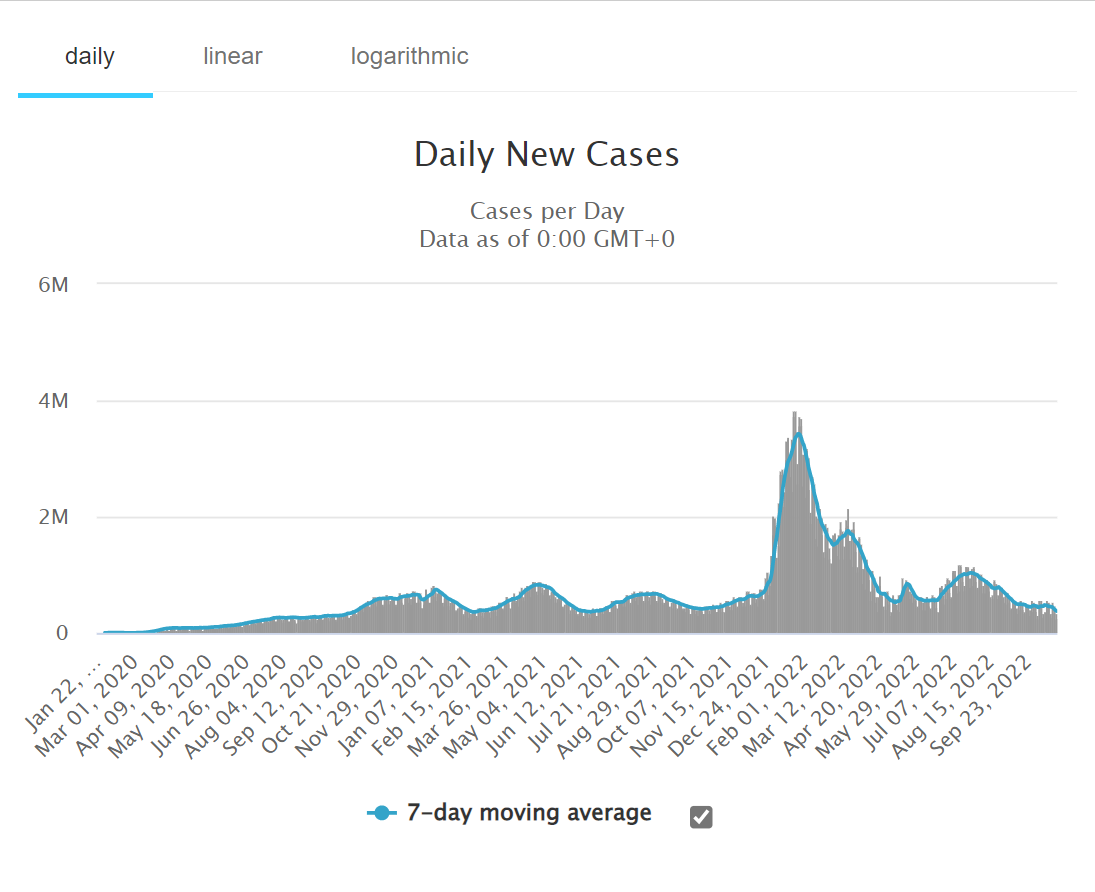
\includegraphics[scale=0.5]{Peta_sebaran.png}
    \caption{Gambar Pertambahan Kasus \covid\ Dunia\cite{a3}.}
    \label{fig:Ch01_denah}
\end{figure}
Sejak kasus \covid\ muncul pada tahun 2019, pandemi ini menyebar dengan cepat hingga terdapat 633.047.720 kasus tercatat pada tanggal 24 Oktober 2022 yang telah dicatat di seluruh negara. Terdapat 6.583.622 kasus kematian dengan 612.165.538 angka pasien yang sembuh. 
Gambar \ref*{fig:Ch01_denah} menunjukkan grafik pertambahan kasus \covid\ setiap hari sejak tanggal 30 Januari 2020 hingga 23 September 2022. Warna hitam menunjukkan angka pertambahan setiap hari sedangkan garis warna biru menunjukkan \textit{7-day moving average} untuk memperlihatkan angka pertambahan kasus baru dan kecepatan pertumbuhannya yang dihitung dari hari data diambil, 3 hari setlah data diambil, dan 3 hari sebelum data diambil. Masih banyak pertambahan kasus yang terjadi hingga saat ini dan kini \covid\ telah menyebar hingga 228 negara. Terkumpul data bahwa untuk kasus aktif saat ini mencapai 14.298.560 dan angka pasien sembuh 618.749.160. Jumlah kematian total hingga saat ini adalah 6.583.622 yang berarti tingkat kematian dari virus ini adalah $1\%$\cite{a4}. 
%https://www.worldometers.info/coronavirus/

\begin{figure}[H]
        \centering
        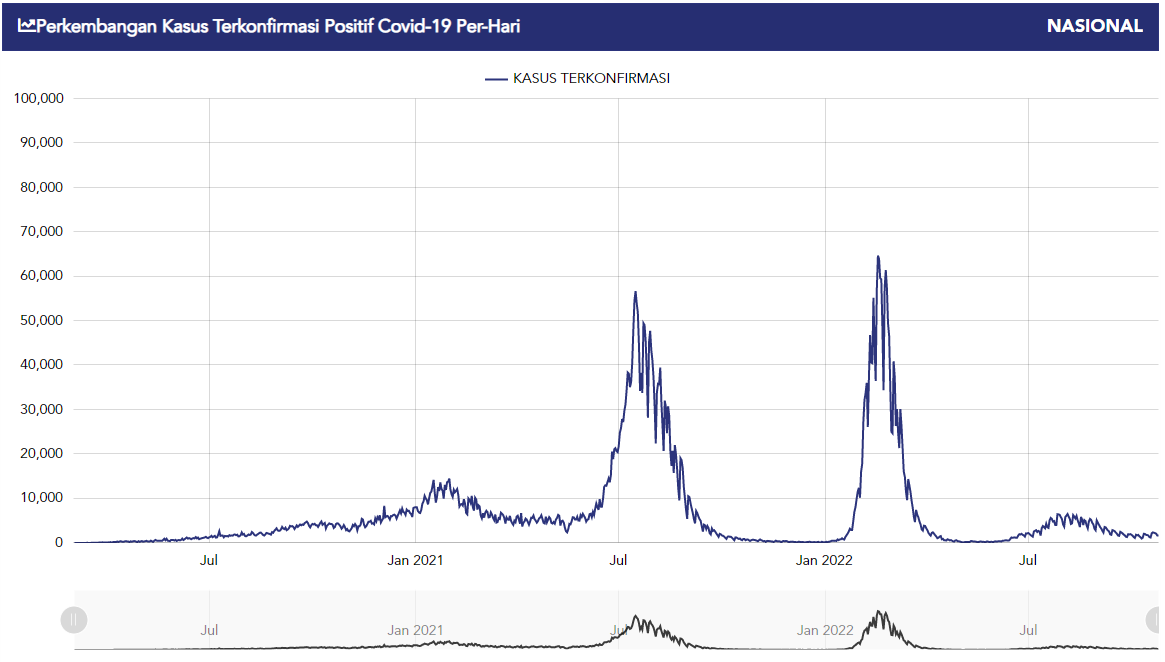
\includegraphics[scale=0.5]{kasus_indo.png}
        \caption{Gambar Perkembangan Kasus \covid\ Indonesia\cite{a1}.}
        \label{fig:Ch01_Indonesia}
    \end{figure}

Pada tanggal 25 November 2022, jumlah kasus tercatat di Indonesia telah mencapai 6.472.664 jiwa dengan jumlah sembuh 6.295.525 dan jumlah meninggal 158.454\cite{a3}. Pada grafik perkembangan yang ditunjukkan Gambar \ref{fig:Ch01_Indonesia}, terlihat pertambahan kasus setiap hari di Indonesia sejak Maret 2021 hingga 25 November 2022. Awal tahun 2022 masih terdapat penambahan yang tinggi hingga 60.000 kasus dalam satu hari. Pada bulan Oktober, jumlah pertambahan kasus berkisar antara 1.000 hingga 2.000 lebih per hari. 

Jumlah kasus terkonfirmasi setiap harinya di Indonesia sudah mulai mengalami penurunan, namun masih banyak pasien yang masih memerlukan perawatan \covid\ dan masih banyak warga yang memerlukan vaksinasi. Hal ini membuktikan bahwa tenaga kesehatan dan fasilitas kesehatan memiliki peran penting dalam kontribusinya menangani \covid. Pemberian bantuan untuk pasien \covid\ dan tenaga kesehatan merupakan salah satu upaya pokok dalam menekan jumlah kasus \covid\ di Indonesia.

\section{Dampak \covid\ terhadap Tenaga Kesehatan}
\label{sec:Dampak_Covid_RS}
Tenaga kesehatan menjadi salah satu garda terdepan dalam penanganan \covid. Meledaknya jumlah pasien COVID-19 membuat berbagai rumah sakit kewalahan karena kekurangan sumber daya salah satunya jumlah tenaga kesehatan yang melayani. Perbedaan yang signifikan antara jumlah pasien dan jumlah tenaga kesehatan ini menyebabkan kelelahan pada tenaga kesehatan karena terlalu banyak bekerja. Tenaga kesehatan juga merupakan pihak yang paling rentan untuk tertular COVID-19 dikarenakan banyaknya kontak langsung terhadap pasien COVID-19. 

\begin{figure}[H]
    \centering
    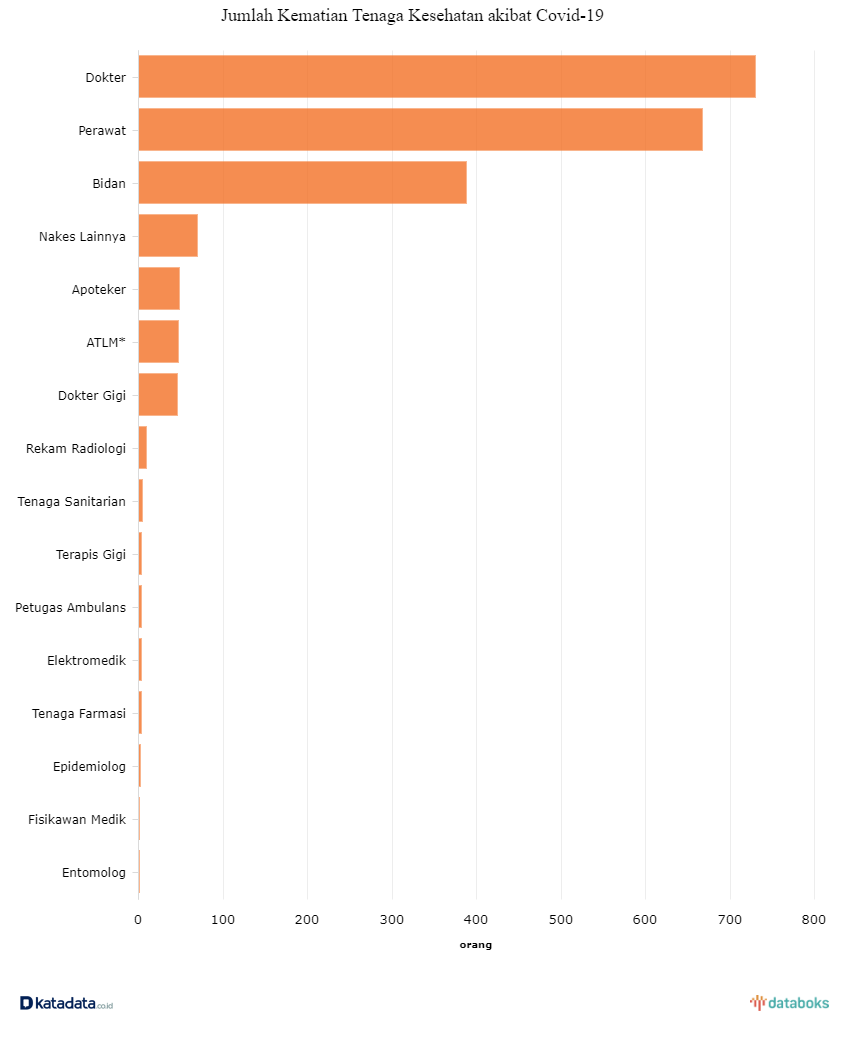
\includegraphics[scale=0.4]{sebanyak-2029-tenaga-kesehatan-meninggal-akibat-covid-19-by-katadata.png}
    \caption{Jumlah Kematian Tenaga Kesehatan Akibat \covid\cite{a6}.}
    \label{fig:Ch01_sebaran_nakes}
\end{figure}

WHO memperkirakan antara 80.000 hingga 180.000 tenaga kesehatan meninggal karena COVID-19 pada periode antara Januari hingga Mei tahun 2020\cite{a5}. Jumlah ini didapatkan dari total 3,45 juta kasus kematian COVID-19 yang dilaporkan ke WHO pada Mei 2021, namun jumlah kasus sebenarnya diduga lebih tinggi 60\% daripada jumlah kematian yang dilaporkan ke WHO. Gambar \ref{fig:Ch01_sebaran_nakes} menunjukkan data yang diperoleh di Indonesia yang menyatakan bahwa pada tanggal 15 September 2021 terdapat 2.029 tenaga kesehatan meninggal akibat \covid\ termasuk 730 dokter dan 667 perawat\cite{a6}.

Pandemi COVID-19 telah memengaruhi tenaga kesehatan secara fisik dan psikologi\cite{a7}.
% https://www.weforum.org/agenda/2020/04/10-april-who-briefing-health-workers-covid-19-ppe-training/
Tenaga kesehatan lebih rentan terjangkit \covid\ daripada masyarakat umum karena lebih sering berkontak dengan pasien. Situasi ini membuat berbagai upaya dibentuk untuk meringankan beban yang ada, termasuk dalam bidang teknologi. Automasi rumah sakit menjadi salah satu inovasi yang dikembangkan untuk mengelola rumah sakit dan fasilitas kesehatan, terutama di saat krisis seperti ini.


% Under such dire circumstances, smart technology adoptions and tech enabled tools can come to the rescue to not only help streamline operations but to also drive efficiency and reduce the burden.

% Hospital automation, or RPA is one such tech innovation that can be of immense help for managing hospitals and healthcare facilities, especially in times of such crisis. From scheduling of doctors and nursing staff, assigning beds or rooms, scheduling OR and consulting room assignments to creating and maintaining a patient treatment record, managing out patients and, especially during COVID, manage the testing and vaccination rush, automate reports and send reminders and appointments for regular patient visits.

\section{Bidang Robotika untuk \covid}
\label{sec:Robotika_covid}
Banyak solusi dan teknologi yang dikembangkan untuk memerangi pandemi ini termasuk dalam bidang robotika. Robot \covid\ dikembangkan dengan tujuan salah satunya untuk menjadi asisten tenaga kesehatan. Robot memiliki keuntungan yaitu dapat bekerja dalam jangka waktu yang lama, melakukan kontak dengan pasien dengan aman, dan meningkatkan efisiensi kerja tenaga kesehatan. Dalam memenuhi tugas ini, robot memerlukan kemampuan dasar untuk mengidentifikasi manusia dan membedakannya dengan benda sekitar. Setelah memiliki kemampuan tersebut, robot kemudian dapat dikembangkan lebih lanjut agar dapat menjalankan berbagai tugas.

\begin{figure}[H]
    \centering
    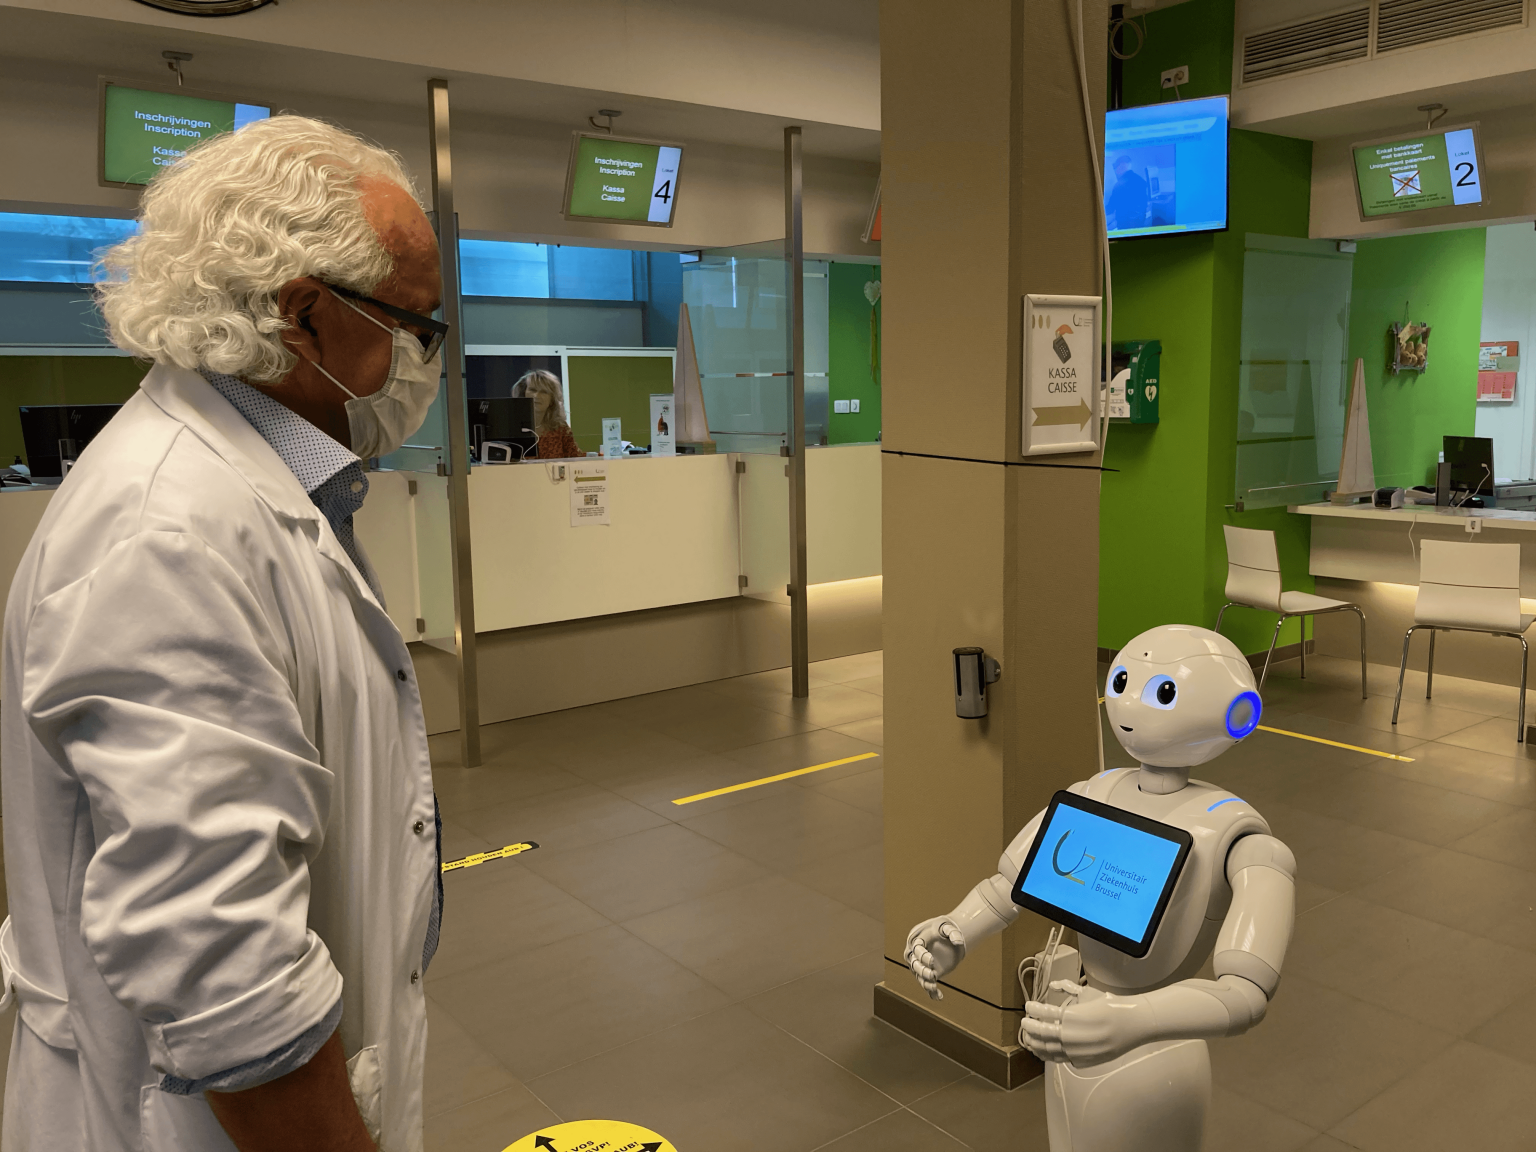
\includegraphics[scale=0.3]{robot_cruzr.png}
    \caption{Robot \textit{Autonomous} CRUZR di Rumah Sakit Belgium\cite{a9}.}
    \label{fig:Ch02_robot_CRUZR}
\end{figure}

Saat ini robot \auto\ juga mulai dikembangkan dalam bidang kesehatan karena dapat memberikan berbagai keuntungan seperti aman, andal, dan mampu untuk memproduksi obat secara efisien\cite{a8}. Gambar \ref{fig:Ch02_robot_CRUZR} merupakan salah satu robot bidang kesehatan yang telah dikembangkan adalah robot CRUZR yang bekerja di \textit{Antwerp University Hospital} di Belgium\cite{a9}. Robot ini mempunyai tugas untuk menyapa pasien, mengecek suhu tubuh dan masker pasien, kemudian mengantar pasien ke ruang yang ingin dituju. Robot ini beroperasi secara mandiri tanpa operator manusia. Hal ini memberikan kelebihan yaitu berkurangnya kontak antara tenaga kesehatan dengan pasien pada masa pandemi \covid\ ini.

\begin{figure}[H]
    \centering
    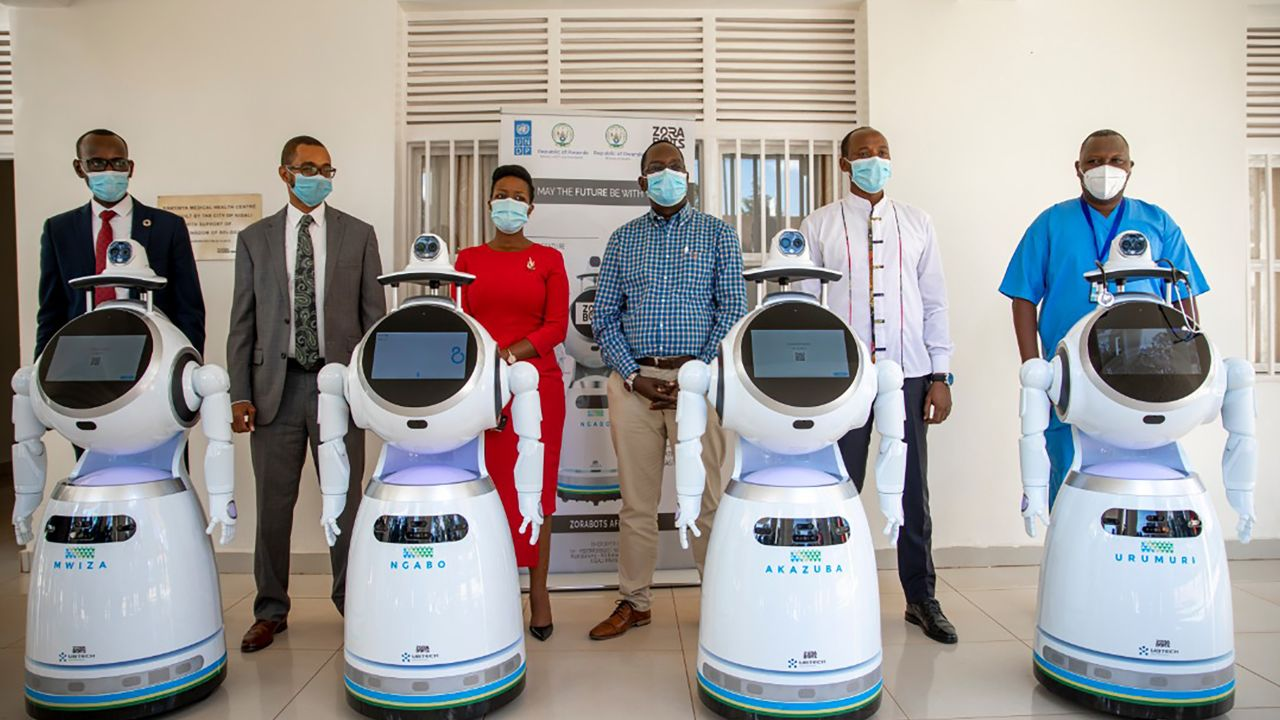
\includegraphics[scale=0.26]{robot_rwanda.jpg}
    \caption{Robot Pelayan Pasien \covid\ di Afrika \cite{a10}.}
    \label{fig:Ch02_robot_rwanda}
\end{figure}
    

Gambar \ref*{fig:Ch02_robot_rwanda} menunjukkan robot-robot pelayan pasien \covid\ dari United Nations Development Program (UNDP) untuk Kanyinya sebagai robot pelayan pasien \covid\ di Kigali, Afrika. Robot-robot tersebut bernama Akazuba, Ikirezi, Mwiza, Ngabo, and Urumuri yang bertugas untuk membantu perawatan pasien. Robot-robot ini dapat melakukan pemindaian suhu massal, pemantauan status pasien, dan penyimpanan rekam medis pasien \covid. Robot juga memiliki kemampuan menangkap data suara dan visual pasien dan dapat memberi tahu petugas kesehatan tentang kelainan yang terdeteksi.
% https://edition.cnn.com/2020/05/25/africa/rwanda-coronavirus-robots/index.html

Pada proyek \textit{capstone} ini dirancang sistem untuk mengembangkan kemampuan robot \covid\ sehingga dapat mengidentifikasi objek manusia dan benda untuk robot \covid. Robot nantinya secara otomatis mampu membedakan objek manusia dengan benda di sekitarnya dari bacaan sensor yang ditanam pada robot. Adanya sistem pendeteksi manusia dan benda ini dapat memberikan solusi untuk pengembangan berbagai kemampuan robot seperti \textit{tracking}, membantu menjadi asistensi tenaga kesehatan, membantu melayani pasien, menggantikan beberapa tugas tenaga kesehatan, hingga menjaga kenyamanan dan keamanan lingkungan rumah sakit. Dengan demikian, robot dapat ikut membantu mengurangi beban kerja tenaga kesehatan dan meningkatkan kualitas pelayanan \covid.

% Bab-bab dalam dokumen C501 ini terdiri dari 11 bab. Bab pertama menjelaskan latar belakang permasalahan yang diangkat. Bab kedua menguraikan dasar teori pendukung yang diperlukan proyek ini. Bab ketiga akan mengenalkan berbagai metode yang dapat menyelesaikan permasalahan. Bab keempat berisi pemodelan matematika dari permasalahan proyek ini. Bab kelima menjelaskan pemilihan metode yang paling tepat untuk menyelesaikan masalah. Bab keenam berisi jenis luaran yang diinginkan beserta spesifikasinya. Bab tujuh menunjukkan batas-batas permasalahan yang diangkat. Bab delapan berisi rancangan umum sistem. Bab sembilan berisi rencana rangka anggaran dan rencana jadwal kegiatan proyek. Bab sepuluh memperlihatkan simulasi awal proyek ini. Bab terakhir yaitu bab sebelas memuat kesimpulan dari rancangan sistem yang akan dibuat dan diimplementasikan.


% BAB 02 : Dasar Teori Pendukung 
\chapter{\uppercase{Dasar Teori Pendukung}}
\label{chap:Dasar_Teori_Pendukung}
%Allahu Akbar

Berbagai penelitian dilakukan untuk mengembangkan sistem deteksi pada robot sejak lama. Proyek \textit{capstone} ini membangun sebuah sistem deteksi manusia dan benda khusus  untuk robot \covid. Robot COVID-19 yang dimaksud pada dokumen ini adalah robot yang dapat bergerak secara otomatis membantu tugas-tugas tenaga kesehatan dan meminimalkan interaksi langsung dari tenaga kesehatan dengan pasien. Sistem ini bertujuan untuk menambah kemampuan robot COVID-19 agar memiliki kemampuan untuk membedakan manusia dengan objek benda mati lainnya yang nantinya berperan menjadi dasar untuk pengembangan fungsi-fungsi lebih lanjut robot dalam membantu tenaga kesehatan.

\section{Robot}
\label{sec:Robot_}

Robot adalah produk dari bidang robotika di mana mesin dapat diprogram dan dibangun untuk membantu manusia atau meniru tindakan manusia. Robot pada awalnya dibangun untuk menangani tugas-tugas monoton (seperti membuat mobil di jalur perakitan pabrik), tetapi semakin lama robot semakin berkembang jauh hingga dapat melakukan tugas-tugas seperti memadamkan api, membersihkan rumah, dan membantu operasi yang sangat rumit. Robot dapat diklasifikasikan menurut jenis lingkungan tempat mereka beroperasi, bidang aplikasi yang dan tugas yang mereka lakukan.

Perbedaan yang paling umum adalah antara robot tetap dan robot bergerak. Kedua jenis robot ini memiliki lingkungan kerja dan membutuhkan kemampuan yang sangat berbeda. Robot tetap sebagian besar berupa manipulator robot industri yang bekerja dalam lingkungan yang disesuaikan untuk robot. Robot industri melakukan tugas berulang tertentu seperti menyolder, merakit, atau mengecat.  Robot ini dapat beroperasi tanpa kehadiran manusia dalam lingkungan tertentu dimana robot harus melakukan tugas dalam
urutan yang ditentukan dan bertindak pada objek yang ditempatkan tepat di depannya.

Robot bergerak merupakan robot yang bergerak dan melakukan tugas-tugas di lingkungan yang besar, tidak jelas, dan tidak pasti yang tidak dirancang khusus untuk robot. Mereka perlu menghadapi situasi yang tidak diketahui secara pasti sebelumnya dan dapat berubah seiring waktu. Contoh robot bergerak adalah penyedot debu robot dan mobil \textit{self-driving}.

\subsection{Jenis-jenis Robot}
\label{sec:Robot_Jenis}

Robot merupakan salah satu solusi untuk meningkatkan produktivitas, meningkatkan keselamatan kerja, dan meningkatkan fleksibilitas di berbagai industri. Inovasi dalam robotika untuk menghasilkan barang dan teknologi baru terus dilakukan agar membuat hidup manusia lebih mudah. Inovasi-inovasi tersebut membuat robot yang muncul saat ini telah memiliki berbagai kemampuan dan bentuk. Robot dapat dikelompokkan menjadi 15 jenis robot yang dapat dilihat pada Gambar \ref*{fig:robot_figures}\cite{b1}.
% https://robots.ieee.org/learn/types-of-robots/

\begin{figure}[H]
    \centering
    \begin{subfigure}[b]{.23\textwidth}
        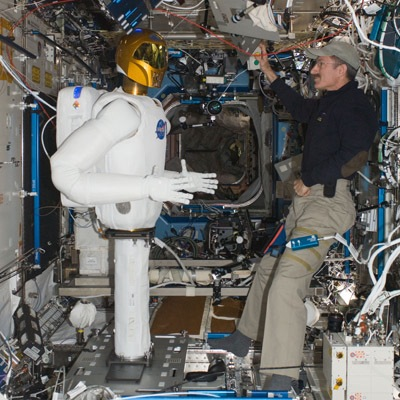
\includegraphics[width=\linewidth]{robot/aerospace.jpg}
        \caption{}
        \label{rob:subfig1}
    \end{subfigure}
    \begin{subfigure}[b]{.23\textwidth}
        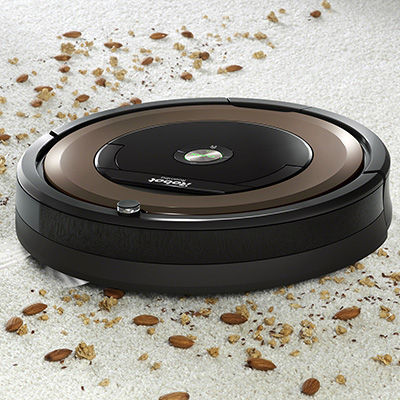
\includegraphics[width=\linewidth]{robot/consumer.jpg}
        \caption{}
        \label{rob:subfig3}
    \end{subfigure}
    \begin{subfigure}[b]{.23\textwidth}
        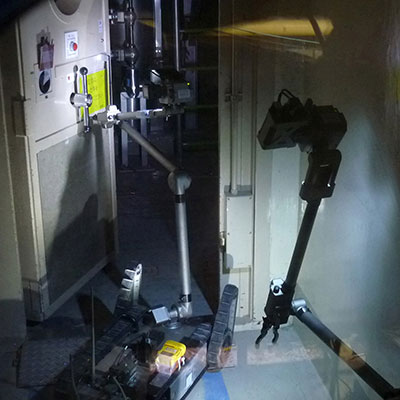
\includegraphics[width=\linewidth]{robot/disasterresponse.jpg}
        \caption{}
        \label{rob:subfig4}
    \end{subfigure}
    \begin{subfigure}[b]{.23\textwidth}
        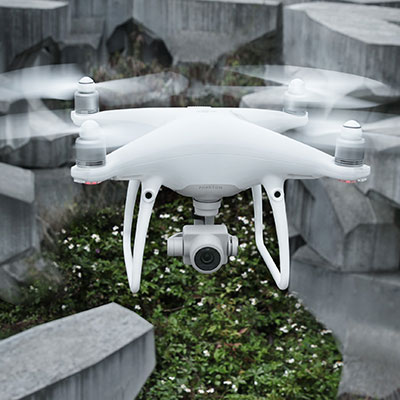
\includegraphics[width=\linewidth]{robot/drones.jpg}
        \caption{}
        \label{rob:subfig5}
    \end{subfigure}
    \begin{subfigure}[b]{.23\textwidth}        
        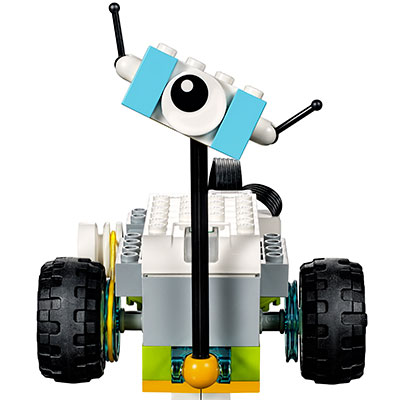
\includegraphics[width=\linewidth]{robot/education.jpg}
        \caption{}
        \label{rob:subfig6}
    \end{subfigure}
    \begin{subfigure}[b]{.23\textwidth}
        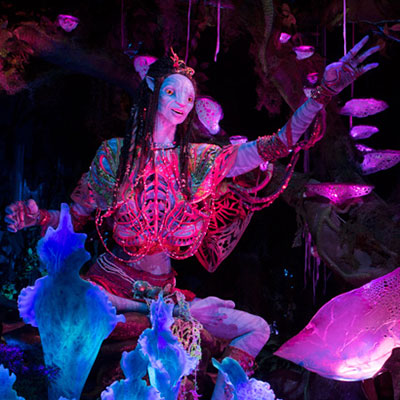
\includegraphics[width=\linewidth]{robot/entertainment.jpg}
        \caption{}
        \label{rob:subfig7}
    \end{subfigure}
    \begin{subfigure}[b]{.23\textwidth}
        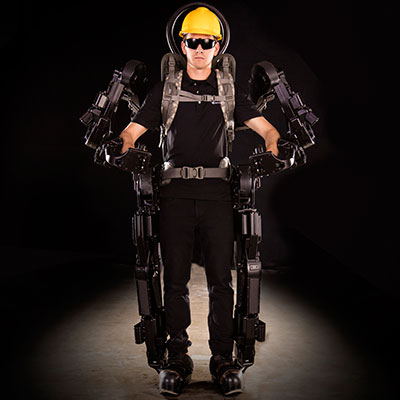
\includegraphics[width=\linewidth]{robot/exoskeleton.jpg}
        \caption{}
        \label{rob:subfig8}
    \end{subfigure}
    \begin{subfigure}[b]{.23\textwidth}
        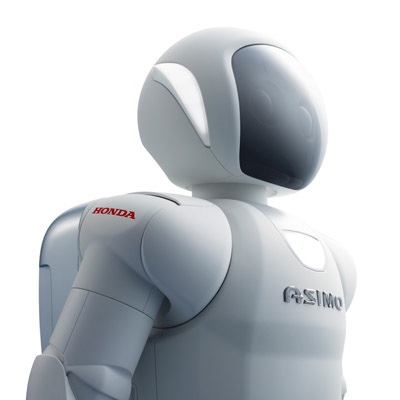
\includegraphics[width=\linewidth]{robot/humanoid.jpg}
        \caption{}
        \label{rob:subfig9}
    \end{subfigure}
    \begin{subfigure}[b]{.23\textwidth}
        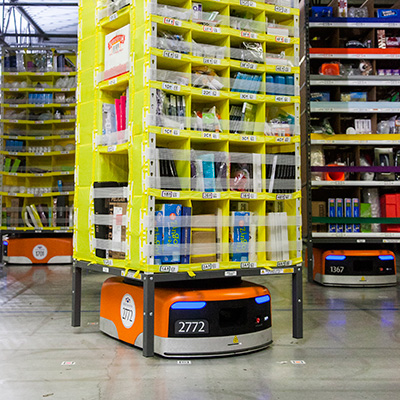
\includegraphics[width=\linewidth]{robot/industrial.jpg}
        \caption{}
        \label{rob:subfig10}
    \end{subfigure}
    \begin{subfigure}[b]{.23\textwidth}
        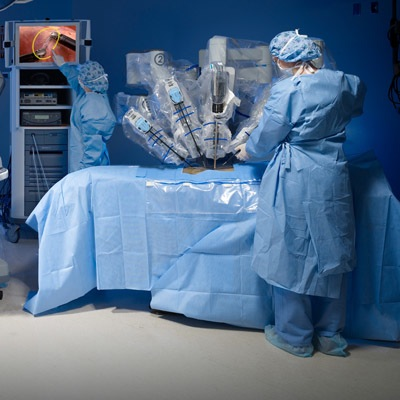
\includegraphics[width=\linewidth]{robot/medical.jpg}
        \caption{}
        \label{rob:subfig11}
    \end{subfigure}
    \begin{subfigure}[b]{.23\textwidth}
        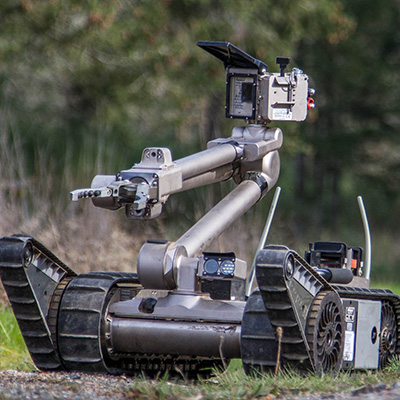
\includegraphics[width=\linewidth]{robot/military.jpg}
        \caption{}
        \label{rob:subfig12}
    \end{subfigure}
    \begin{subfigure}[b]{.23\textwidth}
        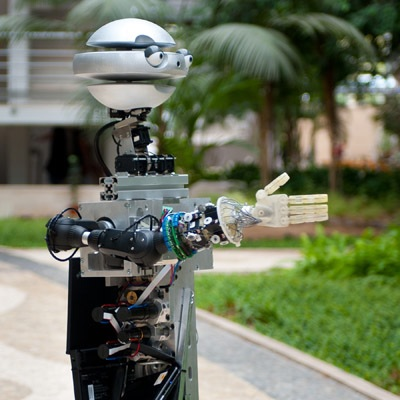
\includegraphics[width=\linewidth]{robot/research.jpg}
        \caption{}
        \label{rob:subfig13}
    \end{subfigure}
    \begin{subfigure}[b]{.23\textwidth}
        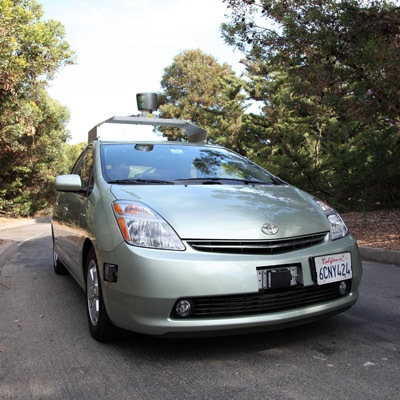
\includegraphics[width=\linewidth]{robot/autonomous.jpg}
        \caption{}
        \label{rob:subfig2}
    \end{subfigure}
    \begin{subfigure}[b]{.23\textwidth}
        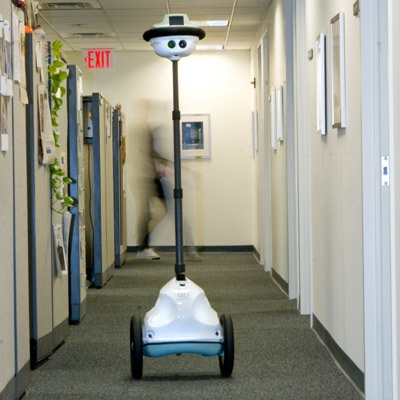
\includegraphics[width=\linewidth]{robot/telepresence.jpg}
        \caption{}
        \label{rob:subfig14}
    \end{subfigure}
    \begin{subfigure}[b]{.23\textwidth}
        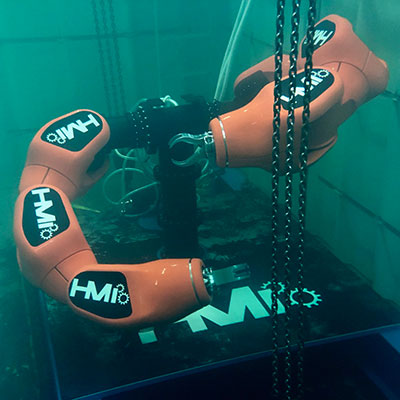
\includegraphics[width=\linewidth]{robot/underwater.jpg}
        \caption{}
        \label{rob:subfig15}
    \end{subfigure}
    \caption{Contoh Jenis-Jenis Robot\cite{b1}.}
    \label{fig:robot_figures}
\end{figure}
Penjelasan mengenai tugas dan fungsi masing-masing jenis robot pada Gambar \ref*{fig:robot_figures} adalah sebagai berikut:
\begin{enumerate}[label=(\alph*)]
    \item \textit{Aerospace}: Kategori \textit{aerospace} mencakup semua jenis robot terbang dan juga robot yang dapat beroperasi di luar angkasa. Pada gambar terlihat robot luar angkasa milik The National Aeronautics and Space Administration (NASA) yang bernama Robonaut. Robot ini memiliki bentuk mirip dengan manusia yang dibuat untuk membantu tugas-tugas astronot di stasiun luar angkasa.
    \item Konsumen: Robot konsumen adalah robot yang dapat dibeli dan digunakan hanya untuk bersenang-senang atau untuk membantu manusia dengan tugas sehari-hari seperti membersihkan ruangan. Gambar menunjukkan salah satu robot yang membantu membersihkan lantai rumah secara otomatis yaitu penyedot debu Roomba.
    \item Tanggap Bencana: Robot-robot ini melakukan pekerjaan berbahaya setelah keadaan darurat. Contoh robot ini tertampil pada gambar yaitu Packbots yang digunakan untuk memeriksa kerusakan di pembangkit listrik tenaga nuklir Fukushima Daiichi setelah gempa bumi dan tsunami melanda Jepang pada tahun 2011.
    \item \textit{Drone}: \textit{Drone} atau disebut kendaraan udara tanpa awak yang digunakan dalam berbagai ukuran untuk menyelesaikan tugas melalui jalur udara. \textit{Drone} memiliki berbagai jenis baling-baling dan ukuran. Gambar menunjukkan \textit{drone} DJI Phantom 4 yang memiliki jenis baling-baling 4 buah atau biasa disebut \textit{drone} \textit{quadcopter}. 
    \item Pendidikan: Kategori robot ini ditujukan untuk generasi peminat robotika berikutnya yang dapat digunakan sebagai bahan pembelajaran di rumah atau di ruang kelas. Robot pada gambar adalah robot Lego WeDo 2.0 yang dapat digunakan sebagai sumber belajar pemrograman pada robot.
    \item Hiburan: Robot-robot ini dirancang untuk membangkitkan respons emosional dan membuat manusia tertawa atau merasa terkejut atau kagum. Salah satu contoh robot hiburan pada gambar adalah Navi Shaman, robot ini milik Disney yang dipasang di taman hiburan mereka. 
    \item \textit{Exoskeleton}: Robot \textit{exoskeleton} adalah robot yang membantu pergerakan tubuh. Robot \textit{exoskeleton} pada gambar adalah robot Ekso yang berfungsi untuk membantu pasien lumpuh. Robot ini juga dapat digunakan untuk rehabilitasi fisik dan untuk memungkinkan pasien yang lumpuh berjalan lagi.
    \item Humanoid: Robot ini menyerupai fisik manusia dan mengerjakan tugas-tugas manusia. Robot humanoid pada gambar adalah robot milik Honda yaitu robot Asimo.
    \item Industri: Robot industri biasanya terdiri dari lengan manipulator yang dirancang untuk melakukan tugas berulang. Kategori ini juga mencakup robot yang bekerja dalam sebuah sistem seperti robot gudang Amazon pada gambar dan robot kolaboratif pada pabrik yang dapat beroperasi bersama pekerja manusia.
    \item Medis: Robot medis dan perawatan kesehatan mencakup sistem seperti robot bedah da Vinci pada gambar, \textit{bionic prostheses} yang menggantikan bagian tertentu fisik manusia, serta \textit{exoskeleton}.
    \item Militer dan Keamanan: Robot yang bekerja pada bidang militer dan keamanan baik untuk membantu manusia maupun menggantikan manusia dalam tugas berbahaya militer dan keamanan. Contoh robot dalam gambar adalah  PackBot dari Endeavor Robotics yang digunakan di Irak dan Afghanistan untuk mencari alat peledak.
    \item Penelitian: Robot yang digunakan duntuk membantu para peneliti melakukan penelitian dan berbagai tugas lainnya. Robot yang ditampilkan pada gambar adalah Flash yang dirancang untuk mengeksplorasi bagaimana manusia merespons sebuah robot yang dapat berbicara, menggerakkan tangan, dan membuat ekspresi wajah.
    \item \textit{Self-Driving Cars}: Robot ini memiliki bentuk kendaraan yang dapat menyetir sendiri secara otomatis. Contoh robot pada gambar yaitu mobil \textit{self-driving} Toyota Prius milik Google. 
    \item \textit{Telepresence}: Robot \textit{telepresence} memiliki kemampuan yang memungkinkan pengguna untuk hadir di suatu tempat tanpa benar-benar pergi ke sana. Contoh robot terlihat pada gambar adalah Anybots QB yang membuat pengguna mampu mengendalikan robot dengan masuk ke avatar robot melalui internet untuk mengendarainya, melihat apa yang dilihatnya, dan berbicara dengan orang-orang sekitarnya.
    \item \textit{Underwater}: Robot yang dibuat khusus untuk beroperasi di bawah air. Terlihat pada gambar yaitu Aquanaut yang dikembangkan Houston Mechatronics yang dapat bertransformasi menjadi kapal selam dan robot setengah humanoid.
\end{enumerate}


\subsection{Robot \textit{Autonomous}}
\label{sec:Robot_Autonomous} 
    
Setiap robot memiliki tingkat otonomi yang berbeda mulai dari robot yang dikendalikan manusia yang melakukan tugas yang dikendalikan sepenuhnya oleh manusia hingga robot yang sepenuhnya \auto\ yang melakukan tugas tanpa perintah eksternal. Robot \auto\ merupakan robot yang mampu memutuskan aksinya untuk mengeksekusi perintah secara mandiri tanpa campur tangan manusia hingga tujuan tercapai\cite{b2}. Robot ini memanfaatkan berbagai sensor untuk memperoleh informasi dan menggunakan hasil pelatihan data untuk memutuskan apa yang akan dilakukan. Robot dapat diklasifikasikan sebagai robot \auto\ jika mereka kemampuan dalam persepsi, pengambilan keputusan dan aksi secara mandiri. Walaupun robot ini tidak memerlukan tenaga manusia saat beroperasi, robot ini masih memerlukan manusia untuk melakukan perawatan secara berkala.

Robot \auto\ saat ini dioperasikan dalam berbagai bidang dalam kehidupan sehari-hari. 
Robot \auto\ biasa digunakan dalam transportasi logistik misal dalam \textit{e-commerce} menggunakan robot \auto\ untuk melakukan transportasi barang, pemenuhan pesanan, penyortiran, dan pengatur penyimpanan. Robot ini juga digunakan untuk mengangkat barang berat dan mengangkut barang ke seluruh ruangan dalam gudang-gudang. 
Robot \auto\ dalam industri umumnya memiliki bagian tambahan khusus seperti lengan dan konveyor untuk memudahkan produksi dan distribusi.
% This also enables instant, accurate, and easily accessible documentation of the process.

\subsection{Robot Bergerak}
\label{sec:Robot_Bergerak}

Robot bergerak merupakan kombinasi dari berbagai macam perangkat keras dan perangkat lunak untuk bergerak di ruang bebas. Robot ini mencakup semua robot yang memiliki kemampuan mobilitas. Robot beroda merupakan bentuk umum yang biasa dijumpai untuk robot bergerak. Gambar \ref*{fig:Ch02_control_scheme} menunjukkan alur kontrol untuk robot beroda. Pertama, robot akan mencari informasi mengenai lingkungan dan mengartikan informasi yang diperoleh. Informasi akan dibuat menjadi peta yang kemudian digunakan untuk menentukan posisi robot dalam peta tersebut atau disebut lokalisasi. Lokalisasi menghasilkan informasi koordinat robot pada ruangan untuk proses selanjutnya yaitu menentukan respon robot sesuai kercerdasan robot (\textit{cognition}). Robot kemudian menentukan jalur yang akan ditempuh selanjutnya dan memberi perintah pada aktuator agar robot bergerak menuju tujuan selanjutnya. 

\begin{figure}[H]
    \centering
    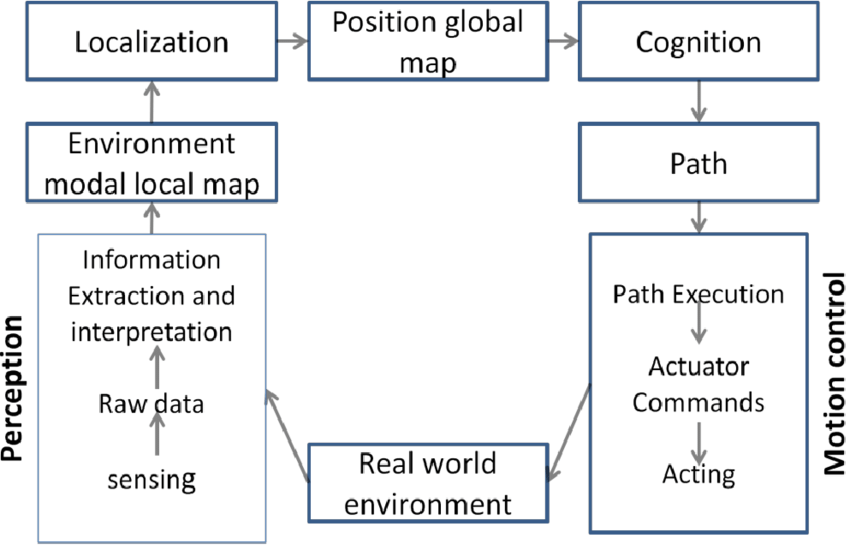
\includegraphics[scale=0.5]{control_scheme.png}
    \caption{Alur Kontrol Robot Beroda \cite{b3}.}
    \label{fig:Ch02_control_scheme}
\end{figure}
% n at: https://www.researchgate.net/publication/267989738

Pada dasarnya, robot bergerak memiliki empat kemampuan dasar yaitu \textit{locomotion, sensing,} kontrol dan komunikasi\cite{b3}. 
\textit{Locomotion} memungkinkan robot bergerak tanpa batas 
di seluruh lingkungannya. 
\textit{Sensing} adalah bagaimana robot mengetahui dan mengukur sifat-sifat dalam dirinya dan lingkungannya.
Kontrol adalah bagaimana robot berpikir untuk menentukan aksi. Komunikasi adalah cara robot mengirim dan menerima pesan dengan robot satu sama lain atau dengan operator. Kemampuan-kemampuan ini memunculkan adanya berbagai macam cara yang robot untuk bergerak dengan pemilihan berbagai macam desain algoritma dan perangkat robot. 

Robot beroda dengan komposisi roda tiga buah merupakan bentuk robot bergerak sederhana yang sering dijumpai pada kehidupan sehari-hari. Gambar \ref*{fig:Ch02_mobile_robot} menunjukkan \textit{base} untuk robot beroda tiga yaitu robot Pioneer 3DX. Roda kanan dan roda kiri adalah sumber gerak robot yang diberi motor robot sedangkan roda \textit{castor} adalah roda penyeimbang robot. Robot bergerak dapat dimodelkan menjadi \textit{physical model} dari badan dan komponen robot seperti pengatur kecepatan, motor, \textit{gearbox}, dsb. 

% Second approach is based on experimental fitting of recorded mobile robot velocity data regarding reference velocity data. 
\begin{figure}[H]
    \centering
    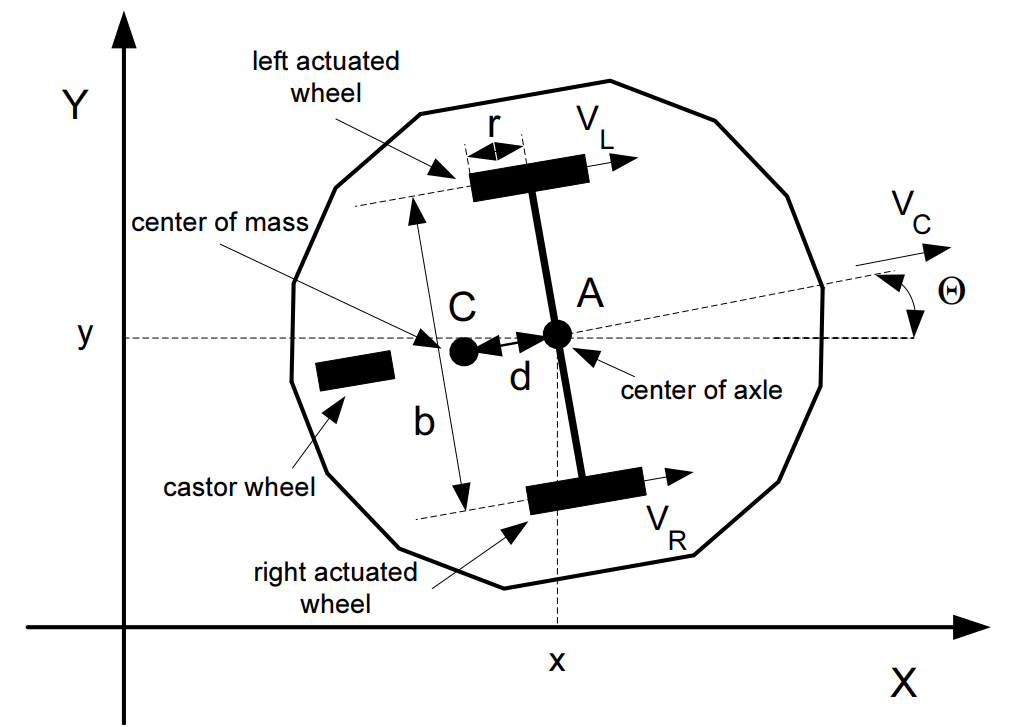
\includegraphics[scale=0.5]{mobile_robot.png}
    \caption{Geometri Robot Pioneer 3DX \cite{b4}.}
    \label{fig:Ch02_mobile_robot}
\end{figure}
% https://www.researchgate.net/publication/228561343_Modelling_of_Mobile_Robot_Dynamics

Gerak lurus robot diproduksi dengan menggerakkan roda kanan dan roda kiri secara bersamaan, sedangkan untuk belok kanan yaitu dengan menaikkan kecepatan roda kiri lebih tinggi dari roda kanan dan sebaliknya untuk belok kiri. Robot ini dapat berputar di tempat dengan menggerakkan satu roda ke depan dan satu ke belakang dari roda kanan dan roda kiri. Roda dilengkapi dengan \textit{encoder} dan sensor pembaca kecepatan untuk mencatat pergerakan robot. Gambar juga menunjukkan komponen-komponen geometri robot antara lain yaitu $r$ sebagai jari-jari roda robot $(mm)$, $v_L$ dan $v_R$ sebagai kecepatan roda kanan dan roda kiri $(mm/s)$, $x$ dan $y$ yang mewakilkan posisi pada koordinat kartesian dalam $(mm)$, dan $b$ adalah jarak antar roda penggerak dalam $(mm)$. Persamaan gerak dinamis robot beroda tiga dapat diturunkan menggunakan formula Euler-Lagrange\cite{b4} pada persamaan \ref*{eq:aeuler_lagrange}:
\begin{equation}
    \glsadd{diferensial_biasa}\glsadd{diferensial_p}
    \diff{}{t}\left(\diffp{L}{\dot{q}_i}\right)-\frac{L}{q_i}=Q_i
    \label{eq:aeuler_lagrange}
\end{equation}
\begin{tabbing}
    dengan: \=\\
        \>$L$ \qquad \=: perbedaan energi kinetik $(T)$ dan energi potensial $(U)$,\\ 
        \>$q_i$ \>: koordinat umum $\bar{x}=\frac{1}{N}\sum_{i=1}^n x_i$,\\
        \>$Q_i$ \>: gaya yang bekerja pada sistem mekanik.
\end{tabbing}
Robot diasumsikan hanya bergerak pada permukaan datar sehingga energi potensial robot adalah nol $(U = 0)$. Persamaan \ref*{eq:aeuler_lagrange} dapat ditulis ulang menjadi persamaan \ref*{eq:euler_lagrange2a} dan persamaan \ref*{eq:euler_lagrange2b}.
\begin{align}
    \label{eq:euler_lagrange2a}
    \glsadd{diferensial_biasa}\diff{}{t}\left(\glsadd{diferensial_p}\diffp{L}{\dot{\Theta}_R}\right)-\glsadd{diferensial_p}\diffp{L}{\Theta_R}=M_R-K\dot{\Theta}_R,\\
    \label{eq:euler_lagrange2b}
    \diff{}{t}\left(\glsadd{diferensial_p}\diffp{L}{\dot{\Theta}_L}\right)-\glsadd{diferensial_p}\diffp{L}{\Theta_L}=M_L-K\dot{\Theta}_L.
\end{align}
\begin{tabbing}
dengan: \=\\
        \>$\Theta_R$ \qquad \=: posisi sudut roda kanan $(rad)$,\\ 
        \>$\Theta_L$ \qquad \>: posisi sudut kiri $(rad)$,\\
        \>$\dot{\Theta}_R$ \>: kecepatan angular roda kanan $(rad/s)$,\\
        \>$\dot{\Theta}_L$ \>: kecepatan angular roda kiri $(rad/s)$,\\
        \>$M_R$ \>: torsi roda kanan $(kgmm/s^2)$,\\
        \>$M_L$ \>: torsi roda kiri $(kgmm/s^2)$,\\
        \>$K\dot{\Theta}_R$ \>: nilai gaya gesek viskos roda kanan $(kgmm/s^2)$,\\
        \>$K\dot{\Theta}_L$ \>: nilai gaya gesek viskos roda kiri $(kgmm/s^2)$,\\
        \>$Q_i$ \>: gaya yang bekerja pada sistem mekanik.
\end{tabbing}
kemudian kedua persamaan di atas dapat ditulis ulang menjadi:
\begin{align}
    \label{eql: 1}
    A\ddot{\Theta}_R+B\ddot{\Theta}_L=M_R-K\dot{\Theta}_R,\\
    \label{eql: 2}
    B\ddot{\Theta}_R+A\ddot{\Theta}_L=M_L-K\dot{\Theta}_L.
\end{align}
Persamaan \ref*{eql: 1} dan \ref*{eql: 2} jika dihubungkan dengan variabel-variabel robot beroda pada Gambar \ref*{fig:Ch02_mobile_robot} akan menghasilkan dua persamaan akhir yaitu:
\begin{align}
    \label{eql: 1a}
    A=\left(\frac{mr^2}{4}+\frac{(I_A+md^2)r^2}{b^2}+I_0\right),\\
    \label{eql: 1b}
    B=\left(\frac{mr^2}{4}-\frac{(I_A+md^2)r^2}{b^2}\right),
\end{align}
\begin{tabbing}
    dengan: \=\\
        \>$m$ \qquad \=: massa seluruh robot $(kg)$,\\ 
        \>$I_A$ \>: momen inersia seluruh robot terhadap titik A $(kgmm^2)$,\\
        \>$I_0$ \>: momen inersia gabungan motor penggerak (rotor) dan roda $(kgmm^2)$.
\end{tabbing}

% Mobile Robot Control on a Reference Path/ https://www.researchgate.net/publication/224616884_Mobile_Robot_Control_on_a_Reference_Path : ngga dipakai

\section{Sensor Persepsi}
\label{sec:sensor}  
    Sensor persepsi adalah sensor yang digunakan untuk mendeteksi dan mengenali objek-objek di sekitar.
    Ada berbagai sensor yang dapat digunakan robot untuk membaca dan memetakan lingkungan sekitar tanpa memerlukan kontak fisik. Sensor-sensor ini dapat bekerja untuk menentukan jarak objek di sekitarnya hingga dapat memberi gambaran bentuk objek target. Jenis sensor robot dapat dibedakan menjadi dua yaitu sensor \textit{proprioceptive} dan sensor \textit{exteroceptive}\cite{b5}. Sensor \textit{proprioceptive} mengukur nilai-nilai internal sistem (robot) seperti kecepatan motor, beban roda, sudut lengan robot, tegangan baterai, dsb. Sensor \textit{exteroceptive} digunakan untuk memperoleh informasi dari lingkungan robot seperti pengukuran jarak, intensitas cahaya, amplitudo suara, dsb. Pada subbab ini akan dijelaskan beberapa contoh sensor persepsi \textit{exteroceptive} yang dapat digunakan untuk mendeteksi posisi objek-objek sekitar robot.
%    https://www.globalspec.com/reference/8277/348308/Chapter-6-Classification-of-Sensors
   
   \subsection{Kamera RGB-D}
    \label{subsec:Sub-Metode_Kamera}
    
    Robot \auto\ biasanya memiliki beberapa kemampuan seperti \textit{Obstacle Avoidance (OA), Augmented Reality (AR), Simultaneous Localization and Mapping (SLAM),} dan \textit{Mobile Object Tracking (MOT)} yang semuanya membutuhkan informasi akurat mengenai posisi objek sekitarnya. Pendeteksian objek menggunakan kamera yang biasanya dapat mengetahui jarak target untuk memperoleh informasi lengkap seperti letak dan tekstur target. Kamera yang memiliki kemampuan tersebut disebut dengan kamera RGB-D (\textit{Red, Green, and Blue - Depth}). Kamera RGB-D memberikan informasi berupa gabungan visual warna, bentuk dan kedalaman untuk mengenali target\cite{b6}. Contoh hasil bacaan kamera RGB-D diperlihatkan pada Gambar \ref{fig:Ch02_rgbd_kamera}.
    \begin{figure}[H]
        \centering
        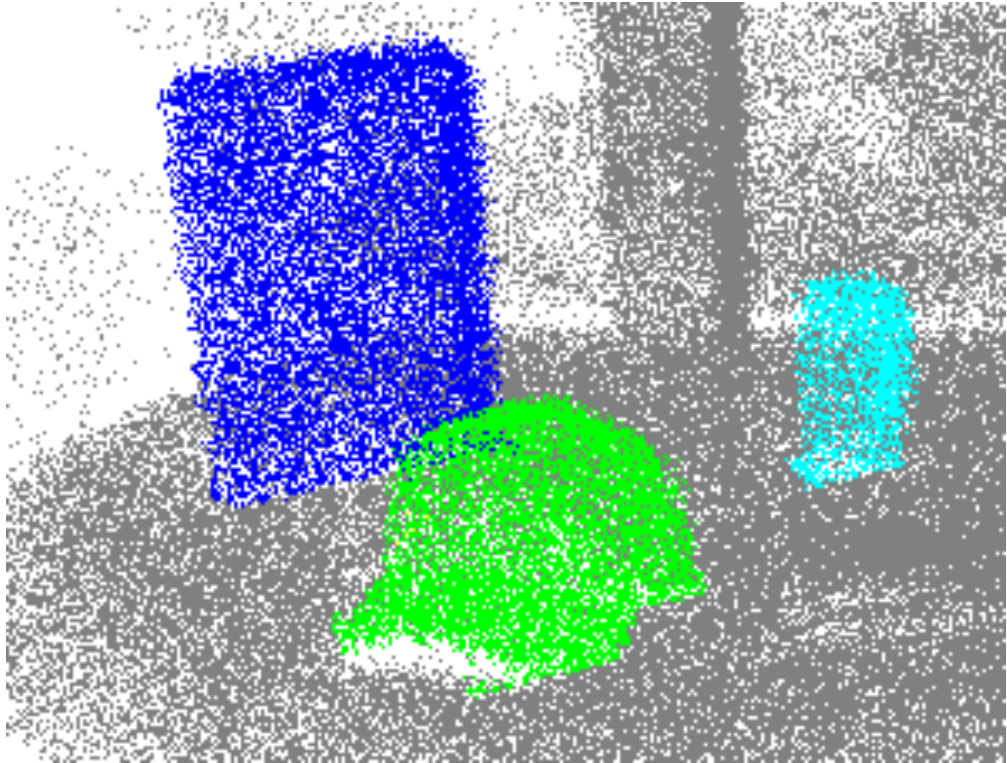
\includegraphics[scale=0.3]{rgbd.png}
        \caption{Contoh hasil bacaan kamera RGB-D\cite{b6}.}
        \label{fig:Ch02_rgbd_kamera}
    \end{figure}

    % https://www.researchgate.net/publication/336829539_RGB-D_Image_Analysis_and_Processing : sumber utamaaaaaaaaaaaa bab di bawah
    \subsubsection{Jenis-jenis Kamera RGB-D}
    \label{subsec: jenis_rgb_d}
    Kamera yang digunakan secara aktif memodifikasi \textit{scene} untuk menyederhanakan masalah rekonstruksi dapat dimasukkan dalam sensor aktif. Ada dua jenis kelas kamera sensor aktif  yang didasarkan pada prinsip kerja yang berbeda, yang disebut kamera \textit{Time of Flight} (ToF) dan \textit{Structured Light} (SL)\cite{b7}.
    % Sarbolandi H, Lefloch D, Kolb A (2015) Kinect range sensing: structured-light versus time of-flight kinect. Comput Vis Image Underst 139:1–20. https://doi.org/10.1016/j.cviu.2015.05.006
    Kamera SL memproyeksikan pola unik ke dalam \textit{scene} untuk menambahkan fitur tambahan untuk menyederhanakan pencocokan fitur dan perhitungan kedalaman (\textit{depth}). Tantangan yang dihadapi pendekatan rekonstruksi ini adalah ketika ada wilayah tanpa fitur pada \textit{scene}. Sementara itu, kamera ToF bekerja dengan  memancarkan pulsa cahaya (dapat yang sudah termodulasi) dan mengukur waktu perjalanan pulang pergi pulsa atau pergeseran fase. Sensor moderen untuk kedua kasus tersebut biasanya bekerja dalam domain inframerah (IR) agar tidak mengganggu penglihatan manusia dan memungkinkan penangkapan penampilan pemandangan secara simultan.

    \paragraph{Kamera \textit{Time of Flight}}
    \label{subsec: kamera_tof}
    Prinsip kerja dasar kamera ToF didasarkan pada pengukuran waktu pulsa cahaya yang dipancarkan hingga dipantulkan kembali\cite{b8}.
    % Foix S, Alenya G, Torras C (2011) Lock-in time-of-flight (ToF) cameras: a survey. IEEE Sens J 11(9):1917–1926. https://doi.org/10.1109/JSEN.2010.2101060
    Ada dua jenis kamera TOf. Jenis pertama yaitu kamera \textit{Pulsed Time-of-Flight}, mengukur waktu perjalanan pulang pergi(\textit{round trip time}) dari pulsa cahaya yang dihitung dari kecepatan \textit{shutters} dan kecepatan \textit{clock}. Jarak perjalanan pulang pergi dapat dihitung dengan mengukur keterlambatan antara pengiriman dan penerimaan pulsa cahaya. \textit{Scene depth} dapat dihitung sebagai setengah dari jarak perjalanan pulang pergi yang diukur yaitu:
    \begin{equation}
        \textit{Depth} = \frac{\textit{Speed\ of\ Light}\times \textit{Round\ Trip\ Time}}{2}.
    \end{equation}
    Jenis kedua kamera ToF menggunakan pulsa cahaya yang termodulasi waktu kemudian mengukur pergeseran fase antara pulsa yang dipancarkan dan yang kembali. Pulsa cahaya biasanya dimodulasi oleh gelombang kontinu. Detektor fase digunakan untuk memperkirakan fase pulsa cahaya yang kembali. Setelah itu, \textit{scene depth} diperoleh dengan korelasi antara pergeseran fase dan \textit{scene depth}. Teknik multi-frekuensi dapat digunakan untuk lebih meningkatkan akurasi pengukuran kedalaman yang diperoleh dan rentang pengindraan efektif kamera. Contoh kamera ToF jenis ini adalah Microsoft Kinect One dan Creative Senz3D.

    \paragraph{Kamera \textit{Structured Light}}
    \label{subsec: kamera_sl}
    Jenis kamera SL memiliki cara kerja mirip dengan rekonstruksi stereo yaitu didasarkan pada triangulasi. Konsepnya adalah mengganti salah satu dari dua kamera dalam sistem stereo dengan proyektor. Proyektor dapat diartikan sebagai kamera terbalik. Proyeksi pola terstruktur unik yang diketahui [14] ke dalam \textit{scene} menyebabkan fitur buatan tambahan diperkenalkan ke dalam \textit{scene}. Beberapa sensor (seperti Microsoft Kinect) memproyeksikan pola titik unik [4] dan beberapa sensor lain memproyeksikan urutan temporal garis-garis hitam dan putih. Kamera SL tersebar luas dan sering digunakan dalam penelitian. Sensor komoditas dari kategori ini biasanya bekerja di domain inframerah untuk tidak mengganggu penglihatan manusia dan memungkinkan penangkapan simultan dari gambar warna tambahan. Contoh sensor komoditas berbasis teknologi ini adalah Microsoft Kinect, Primesense Carmine, Asus Xtion Pro, dan Intel Realsense.

    \subsubsection{\textit{Missing Depth}}
    \label{subsec:missing_depth}
    
    Saat ini ada banyak tantangan dalam mengestimasi \textit{scene depth} yang merupakan salah satu bagian mendasar dari setiap sistem penglihatan 3D yang berfokus pada gambar RGB-D.
    Pendekatan \textit{depth-sensing} yang berbeda dapat menyebabkan berbagai masalah dalam kedalaman pemandangan yang diperoleh, sehingga proses penyelesaian dan penyempurnaan \textit{depth} merupakan langkah penting pada langkah pasca-pemrosesan.
    \begin{figure}[H]
        \centering
        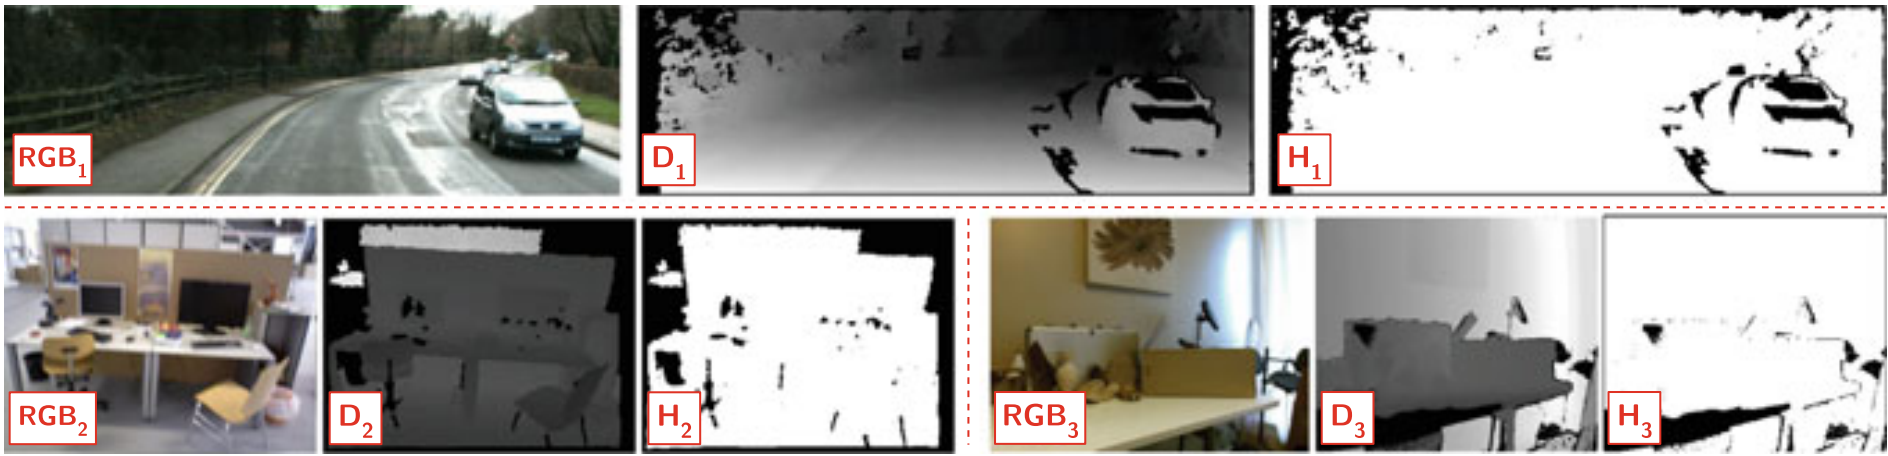
\includegraphics[width=\textwidth]{missing_depth.png}
        \caption{Kedalaman yang Hilang pada Kamera RGB-D\cite{b9}.}
        \label{fig:Ch02_missing_depth}
    \end{figure}

Selain itu, nilai yang hilang kebanyakan berada di \textit{scene} yang berisi wilayah yang tersumbat (kelompok piksel yang terlihat dalam satu gambar tetapi tidak di gambar lain), permukaan tanpa fitur, informasi yang jarang untuk objek pemandangan seperti semak belukar, batas objek yang tidak jelas, objek yang sangat jauh dan sejenisnya. Masalah tersebut dapat dilihat pada Gambar \ref{fig:Ch02_missing_depth}, topeng biner menandai letak nilai \textit{depth} atau kedalaman yang hilang berada dalam disparitas gambar yang dihitung melalui algoritma korespondensi stereo\cite{b9}.  

Perangkat konsumen seperti kamera SL dan kamera ToF adalah sensor \textit{range} aktif yang banyak digunakan untuk berbagai keperluan karena biayanya yang rendah dan ketersediaan yang luas di pasar komersial dengan pengaturan kalibrasi pabrik.
% Additionally, missing values are prevalent in sections of the scene that contain occluded regions ( groups of pixels that are seen in one image but not the other), featureless surfaces, sparse information for a scene object such as shrubbery, unclear object boundaries, very distant objects and alike. 
% Such issues can be seen in Fig. 2.1 (top), wherein the binary mask marks where the missing depth values are in a disparity image calculated via a stereo correspondence algorithm [65]. On the other hand, consumer devices such as structured light and time-of-flight cameras are active range sensors that are more widely utilized for a variety of purposes due to their low cost and wide availability in the commercial market with factory calibration settings [14, 23, 46].
Namun, karena sejumlah kekurangan seperti gangguan iluminasi eksternal, saturasi cahaya sekitar, deteksi pola cahaya yang tidak akurat dengan adanya gerakan dan \textit{error} jalur cahaya aktif yang disebabkan oleh permukaan reflektif atau oklusi, perangkat SL dapat menghasilkan \textit{depth} yang hilang atau nilai \textit{noise} yang paling baik ditangani dengan penghapusan dan pengisian.
% However, due to a number of shortcomings such as external illumination interference [23], ambient light saturation [46], inaccurate light pattern detection in the presence of motion [125] and active light path error caused by reflective surfaces or occlusion [126], consumer structured light devices can result in missing depth or noisy values that are best handled by removal and subsequent filling.
%
% 2.3.1 RGB Image Inpainting 
\paragraph{RGB Image Inpainting}
\label{paragraf: rgb_inpainting}

\textit{Inpainting} atau pengecatan berkaitan dengan penyelesaian masalah pada wilayah target dalam gambar yang muncul akibat dari penghapusan bagian tertentu dari \textit{scene}. Pendekatan awal \textit{inpainting} adalah berusaha untuk secara mulus menyebarkan isofop (garis dalam gambar dengan nilai intensitas yang sama) ke dalam area target ini.
% Inpainting deals with the issue of a plausibly completing a target region within the image often created as a result of removing a certain portion of the scene. Early image inpainting approaches attempted to smoothly propagate the isophotes (lines within the 
Namun, sebagian besar pendekatan pengecatan gambar cenderung mengabaikan aspek penting yang signifikan bagi rasa masuk akal pengamat yang merupakan komponen spasial frekuensi tinggi dari gambar atau tekstur.
Akibatnya, teknik \textit{inpainting} mulai memasukkan ide-ide dari bidang sintesis tekstur (dimana tujuannya adalah untuk menghasilkan wilayah tekstur besar dari sampel tekstur yang lebih kecil tanpa artefak pengulangan yang terlihat di wilayah yang lebih besar) ke dalam proses \textit{inpainting} untuk mengimbangi kurangnya tekstur yang biasa ditemukan di wilayah target setelah selesai.
% However, most of these approaches [15, 133] tend to ignore an important aspect significant to an observer's sense of plausibility, which is the high-frequency spatial component of the image or texture. 

    \begin{figure}[H]
        \centering
        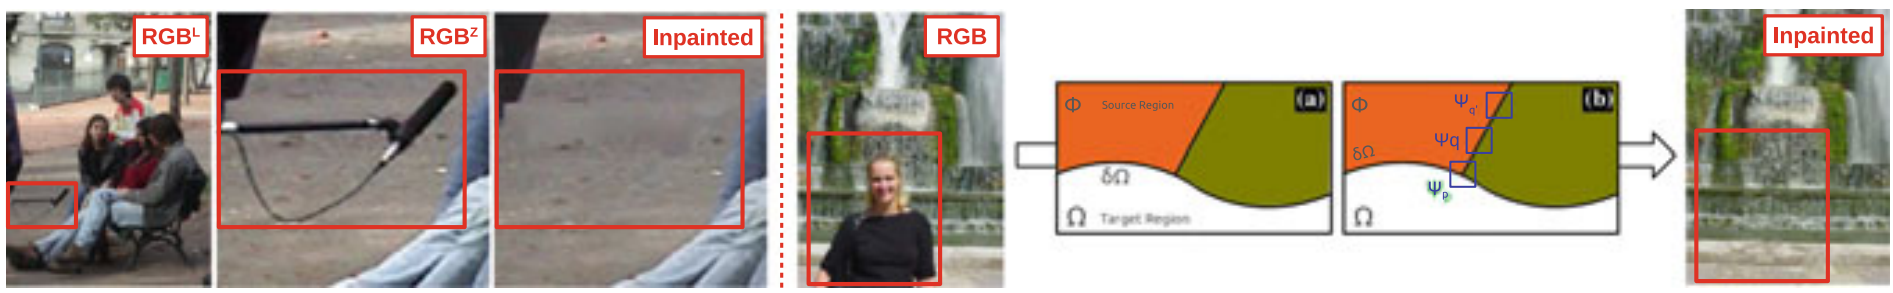
\includegraphics[width=\textwidth]{inpainting.png}
        \caption{Hasil \textit{Inpainting} pada Kamera RGB-D\cite{b9}.}
        \label{fig:Ch02_inpainting}
    \end{figure}


Metode tradisional sintesis tekstur berbasis exemplar diterapkan dengan memprioritaskan urutan pengisian berdasarkan kekuatan gradien di sepanjang batas wilayah target\cite{b10}. 
% In one such approach, the authors of [36] follow traditional exemplar-based texture synthesis methods [43] by prioritizing the order of filling based on the strength of the gradient along the target region boundary. Although the authors of [36] are not the first to carry out inpainting via exemplar-based synthesis [16], previous approaches are all lacking in either structure propagation or defining a suitable filling order that could prevent the introduction of blurring or distortion in shapes and structures. 
Metode berbasis exemplar ini tidak hanya mampu menangani tekstur dua dimensi tetapi juga dapat secara masuk akal menyebarkan struktur linier di dalam gambar. Contoh hasil metode ini dapat dilihat pada Gambar \ref*{fig:Ch02_inpainting}, dimana tekstur air telah disintesis secara masuk akal setelah orang tersebut dikeluarkan dari gambar. Gambar sebelah kiri menunjukkan hasil mikrofon bagian depan telah dihapus dan dicat, tetapi teksturnya tidak akurat dan menyebabkan persepsi kabur. Gambar kanan menunjukkan contoh hasil dan proses pengecatan berbasis exemplar.
Namun, pendekatan ini tidak dapat mengatasi struktur melengkung dan sangat tergantung pada keberadaan lingkungan piksel serupa di wilayah yang dikenal untuk penyelesaian yang masuk akal sehingga beberapa pendekatan lain juga dikembangkan untuk teknik \textit{inpainting}.
% This exemplar-based method [36] is not only capable of handling two-dimensional texture but can plausibly propagate linear structures within the image. An example of the results of this method can be seen in Fig. 2.2 (right), in which water texture has been plausibly synthesized after the person is removed from the image. However, this approach cannot cope with curved structures and is heavily dependent on the existence of similar pixel neighbourhoods in the known region for plausible completion.

% 2.3.2 Depth Filling
\paragraph{\textit{Depth Filling}}
\label{paragraf: depth_filling}

Berbagai teknik \textit{depth filling} yang memanfaatkan teknik-teknik pendekatan \textit{inpainting} juga akan meninggalkan bekasnya pada bagian \textit{depth filling}. Misalnya, penghapusan objek dan \textit{depth filling} gambar RGB-D dilakukan dengan menguraikan gambar menjadi komponen frekuensi spasial tinggi dan rendah yang terpisah melalui filter Butterworth di Fourier Space.
% Nevertheless, just as various depth completion techniques take advantage of other \textit{inpainting} approaches such as [133], with or without modifications [100, 144, 154], exemplar-based image inpainting has also left its mark on depth completion. For instance, in [7], object removal and depth completion of RGB-D images is carried out by decomposing the image into separate high and low spatial frequency components by means of Butterworth filtering in Fourier space. 
Setelah adanya keterikatan gambar frekuensi tinggi dan rendah, informasi frekuensi tinggi (batas objek dan relief tekstur) diisi menggunakan metode sintesis tekstur klasik yang dirumuskan ulang sebagai pendekatan \textit{inpainting} berbasis exemplar piksel demi piksel dan ditingkatkan dengan cara perluasan kueri dalam ruang pencarian, kemudian komponen frekuensi rendah (geometri bentuk yang mendasarinya) diselesaikan melalui \textit{inpainting} berbasis exemplar. Hasilnya  digabungkan kembali dalam domain frekuensi untuk menghasilkan hasil akhir. Hasil dapat dilihat pada Gambar \ref*{fig:Ch02_depth_filling} bahwa gambar yang dihasilkan tajam dan tanpa artefak tambahan. Objek telah dihapus dari gambar RGB-D dan nilai kedalaman yang hilang dalam gambar telah diisi.
% After the disentanglement of high and low frequency images, the high-frequency information (object boundaries and texture relief) is filled using a classic texture synthesis method [43] reformulated as a pixel-by-pixel exemplar-based inpainting approach and enhanced by means of query expansion within the search space, and the low frequency component (underlying shape geometry) is completed via [2]. The results are then recombined in the frequency domain to generate the final output. As can be seen in Fig. 2.5, the produced images are sharp and with no additional artefacts.
\begin{figure}[H]
    \centering
    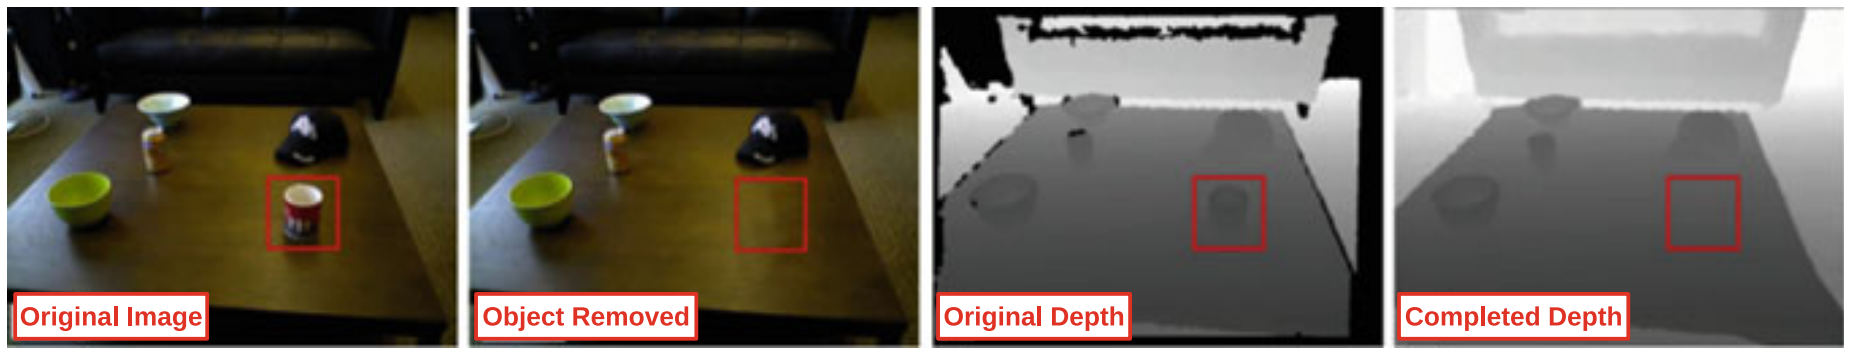
\includegraphics[width=\textwidth]{depth_filling.png}
    \caption{Contoh Hasil \textit{Depth Filling}\cite{b9}.}
    \label{fig:Ch02_depth_filling}
\end{figure}

% Pekerjaan dalam [5] mengembangkan teknik pengecatan RGB dari [36] untuk menciptakan pendekatan berbasis exemplar yang secara eksplisit dirancang untuk melengkapi gambar kedalaman. Ini dicapai dengan menambahkan syarat khusus yang berfokus pada karakteristik gambar kedalaman ke dalam fungsi prioritas untuk menentukan tambalan mana yang diutamakan dalam urutan pengisian. Adanya syarat tekstur dan batas membuat relief permukaan dan tekstur terpelihara dengan baik dalam gambar kedalaman setelah selesai sehingga mengarah ke hasil yang lebih masuk akal dengan artefak yang lebih sedikit. Seperti yang dapat dilihat pada Gambar 2.6, teknik penyelesaian RGB [36] yang diterapkan pada gambar kedalaman menghasilkan banyak artefak yang tidak diinginkan dapat [5] menghasilkan output kedalaman yang lebih tajam.
% The work in [5] extends on the seminal RGB inpainting technique of [36] to create an exemplar-based approach explicitly designed to complete depth images. This is achieved by adding specific terms focusing on the characteristics of depth images into the priority function, which determines which \textit{patch}es take precedence in the filling order. By introducing texture and boundary terms, the authors of [5] ensure that surface relief and texture are well preserved in the depth image after completion, leading to more plausible results with fewer artefacts. As can be seen in Fig. 2.6, the RGB completion technique [36] applied to depth images produces many undesirable artefacts while [5] generates sharper depth outputs.
Pemecahan masalah pengisian kedalaman menggunakan kerangka kerja berbasis exemplar masih memiliki banyak tantangan yang harus dihadapi oleh proses penyelesaian.  Salah satunya jika kedalaman pemandangan bukan dari tampilan \textit{fronto-parallel} maka tidak ada jaminan bahwa nilai kedalaman yang benar dapat diprediksi untuk wilayah yang hilang melalui pengambilan sampel \textit{patch} ketika mencoba menemukan \textit{patch} serupa.
% Even though solving the depth filling problem using an exemplar-based framework has the potential to produce outputs in which structural continuity within the scene is preserved and granular relief texture is accurately and consistently replicated in the missing depth regions, there are still many challenges the completion process must contend with. For instance, if the scene depth is not of a fronto-parallel view, there is no guarantee that correct depth values can be predicted for the missing regions via \textit{patch} sampling even if the \textit{patch}es undergo different transformations such as rotation, scale, shear, aspect ratio, keystone corrections, gain and bias colour adjustments, and other photometric transformations in the search space when trying to find similar \textit{patch}es to sample from [4].
Cara untuk mengatasi masalah ini yaitu dengan penyelesaian matriks yang baru-baru ini muncul sebagai formulasi masalah penyelesaian gambar, terutama setelah diamati bahwa tambalan serupa dalam gambar RGB-D terletak pada subruang dimensi rendah dan dapat diperkirakan oleh matriks dengan peringkat rendah\cite{b11}. Pendekatan dengan matriks menyajikan metode aljabar linier untuk peningkatan gambar kedalaman berbasis penyelesaian matriks peringkat rendah untuk secara bersamaan menghilangkan \textit{noise} dan menyelesaikan gambar kedalaman menggunakan gambar RGB yang sesuai. 

\begin{figure}[H]
    \centering
    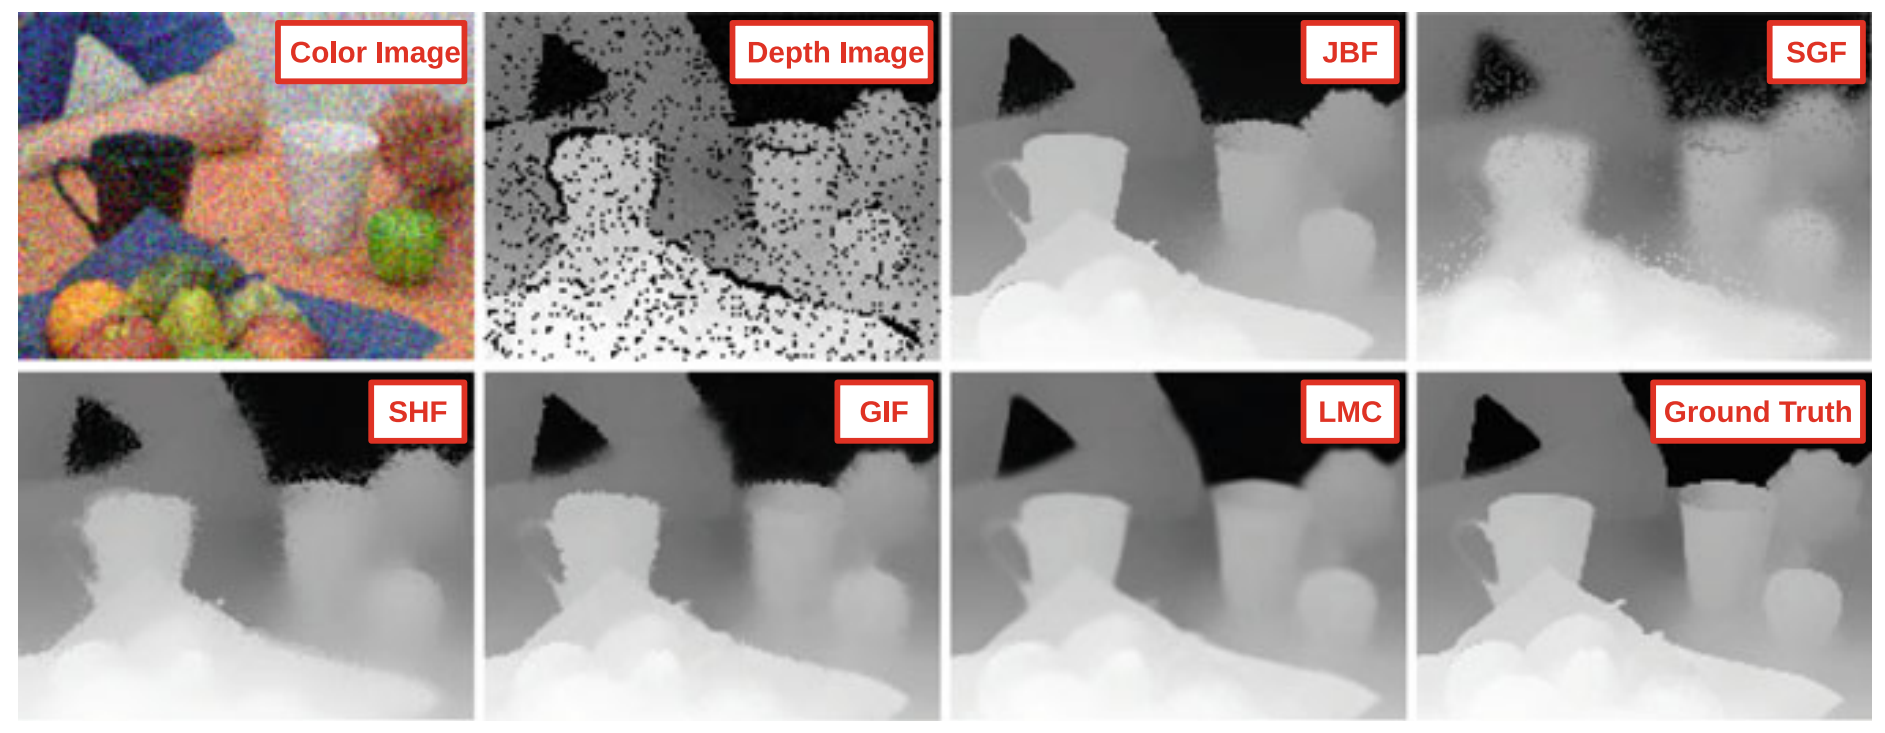
\includegraphics[width=\textwidth]{filling_matriks.png}
    \caption{Contoh Hasil \textit{Depth Filling} Pendekatan Matriks\cite{b9}.}
    \label{fig:Ch02_filling_matriks}
\end{figure}

\textit{De-noising} dan penyelesaian simultan dicapai dengan batasan subruang peringkat rendah yang diberlakukan pada matriks dengan \textit{patch} RGB-D melalui faktorisasi yang tidak lengkap akan
% To combat some of these issues, matrix completion has recently emerged as an interesting formulation of the image completion problem, especially since it has been observed [104] that similar \textit{patch}es in an RGB-D image lie in a low-dimensional subspace and can be approximated by a matrix with a low rank. The approach in [104] presents a linear algebraic method for low-rank matrix completion-based depth image enhancement to simultaneously remove noise and complete depth images using the corresponding RGB images, even if they contain heavily visible noise. In order to accomplish simultaneous de-noising and completion, the low-rank subspace constraint is enforced on a matrix with RGB-D \textit{patch}es via incomplete factorization
menghasilkan penangkapan struktur gambar yang berpotensi bergantung pada pemandangan, baik dari kedalaman maupun ruang warna. Peringkat berbeda dari \textit{patch} ke \textit{patch} tergantung pada struktur gambar, sehingga metode diusulkan untuk secara otomatis memperkirakan nomor peringkat berdasarkan data. Gambar \ref*{fig:Ch02_filling_matriks} menunjukkan kemampuan kinerja pendekatan ini dibandingkan dengan metode penyelesaian kedalaman lainnya seperti \textit{joint bilateral filtering} (JBF), \textit{structure-guided fusion} (SGF), \textit{spatio-temporal hole filling} (SHF) dan \textit{guided inpainting and filtering} (GIF). Pendekatan ini menghasilkan hasil yang bagus walaupun dari input gambar RGB mengandung banyak \textit{noise}.
% which results in capturing the potentially scene-dependent image structures both in the depth and colour space. The rank differs from \textit{patch} to \textit{patch} depending on the image structures, so a method is proposed to automatically estimate a rank number based on the data. Figure 2.7 demonstrates the performance capabilities of this approach compared to other depth completion methods, such as joint bilateral filtering (JBF) [122], structure-guided fusion (SGF) [120], spatio-temporal hole filling (SHF) [25] and guided inpainting and filtering (GIF) [100]. This approach [104] generates particularly impressive results in that the input RGB image is very noisy (Fig. 2.7—Colour Image). Before the comparisons, a de-noising method [37] is applied to the noisy RGB image used as an input for the comparators

 
    \subsection{Sensor Ultrasonik}
    \label{subsec:Ultrasonik}
    Sensor ini memancarkan gelombang ultrasonik untuk mengukur jarak dengan target. Sensor akan menghitung waktu antara pancaran dengan pantulan untuk menghitung jarak. Sinyal ultrasonik memiliki kisaran frekuensi 30 kHz hingga 5 MHz yang dapat digunakan untuk menghasilkan pulsa. Frekuensi tinggi memiliki panjang gelombang yang lebih rendah sehingga resolusi akan menjadi lebih baik, tetapi semakin tinggi frekuensi dapat menghasilkan atenuasi yang juga semakin tinggi. Sensor dengan frekuensi rendah memiliki keuntungan tingkat hamburan rendah dan lebih murah, tetapi panjang gelombangnya di udara hanya beberapa milimeter sehingga memerlukan perawatan khusus\cite{bs1}.
    \begin{figure}[H]
        \centering
        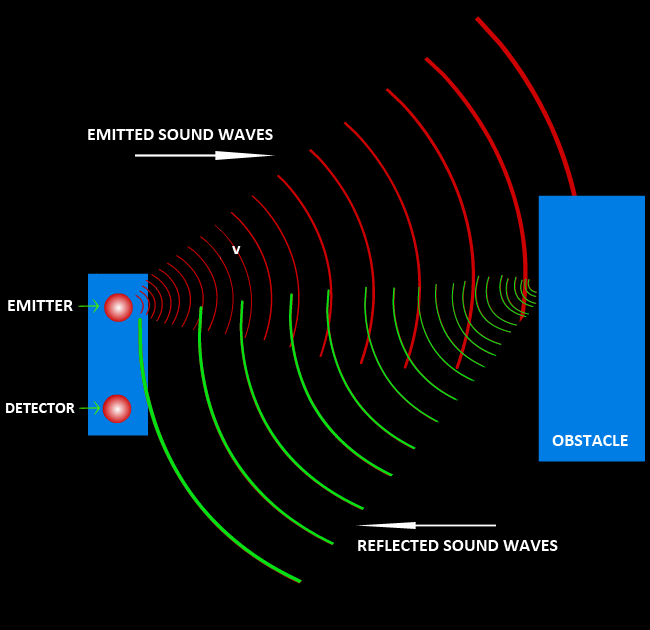
\includegraphics[scale=0.4]{CH02_Ultrasonic.png}
        \caption{Cara kerja sensor ultrasonik\cite{bs2}.}
        \label{fig:Ch02_ultrasonik}
    \end{figure}
    Seperti yang terlihat pada Gambar \ref{fig:Ch02_ultrasonik}, \textit{emitter} pada sensor ini akan memancarkan gelombang dan \textit{detector} akan menangkap gelombang pantul. Gelombang suara ultrasonik yang dikeluarkan adalah getaran pada frekuensi di atas jangkauan pendengaran manusia (\>20kHz) yang dapat merambat melalui berbagai media (udara atau cairan).

    Untuk menghitung jarak antara sensor dan objek, sensor mengukur waktu yang diperlukan antara pengeluaran gelombang oleh pemancar hingga kontaknya dengan penerima. Rumus untuk perhitungan ini adalah 
    \begin{equation}
        D = \frac{1}{2}T * C 
    \end{equation}
    \begin{tabbing}
        dengan : \= \\
        \>D : jarak,\\
        \>T : waktu,\\
        \>C : kecepatan suara (343 meter/detik dalam tekanan standar udara dan suhu 20° C).
    \end{tabbing}

    Sensor ultrasonik digunakan sebagai sensor jarak. Sensor ini dapat ditemukan dalam teknologi parkir mobil otomatis dan sistem keamanan anti-tabrakan. Sensor ultrasonik juga digunakan dalam sistem deteksi rintangan robot, serta teknologi manufaktur. Sensor ultrasonik tidak rentan dibandingkan dengan sensor inframerah (IR) dalam aplikasi pengindraan jarak terhadap gangguan asap, gas, dan partikel udara lainnya (meskipun komponen fisik masih dipengaruhi oleh variabel seperti panas).

    \subsection{Sensor Inframerah}
    \label{subsec:Infrared}

    \begin{figure}[H]
        \centering
        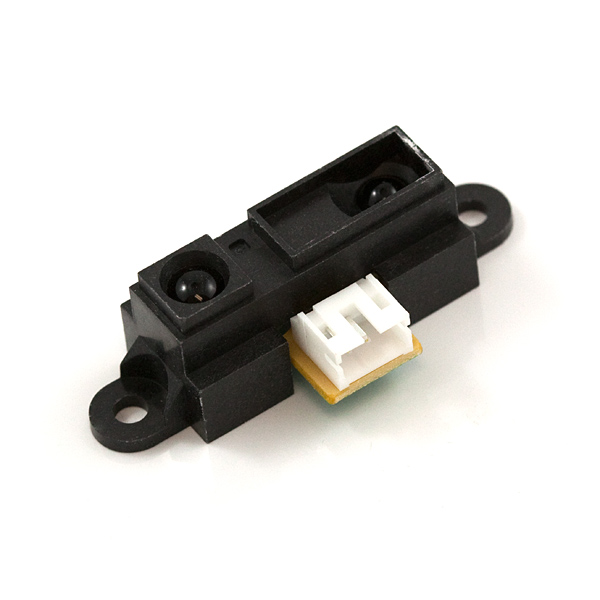
\includegraphics[scale=0.3]{infrared_sensor.jpg}
        \caption{Sensor Jarak Inframerah\cite{bs3}.}
        \label{fig:Ch02_inframerah}
    \end{figure}

    Sensor inframerah (sensor IR) adalah komponen \textit{optoelectronic} yang sensitif terhadap radiasi dengan sensitivitas spektrum dalam rentang panjang gelombang inframerah \SI{780}{\nano\metre} hingga \SI{50}{\micro\metre}\cite{bs4}. 
    Sensor yang terlihat pada Gambar \ref{fig:Ch02_inframerah} tersebut banyak digunakan sebagai detektor gerakan misalnya dalam gedung untuk menyalakan lampu atau dalam sistem alarm untuk mendeteksi penyusup. Sensor mendeteksi radiasi panas (radiasi inframerah) yang berubah seiring waktu dan ruang karena adanya pergerakan. Sensor ini juga banyak digunakan dalam perangkat peringatan gas, penganalisis gas, teknologi pengukuran gas medis, detektor api, dan pengukuran suhu presisi tanpa kontak. 

    Ada dua jenis sensor inframerah yaitu aktif dan pasif\cite{bs5}. Sensor inframerah aktif memancarkan dan mendeteksi radiasi inframerah. Sensor IR aktif memiliki dua bagian yaitu \textit{light-emitting diode} (LED) dan penerima. Objek yang mendekati sensor akan membuat cahaya inframerah dari LED memantul dari objek dan dideteksi oleh penerima. Sensor IR aktif bertindak sebagai sensor jarak, dan biasanya digunakan dalam sistem deteksi rintangan (seperti pada robot). Sensor inframerah pasif (PIR) hanya mendeteksi radiasi inframerah dan tidak memancarkannya dari LED.
    % https://www.researchgate.net/publication/261346136_Application_of_Infrared_sensor_for_shape_detection

    Sensor IR biasanya khusus dibuat sebagai sensor pengukur jarak tipe luaran analog yang terdiri dari light emitting diode (LED) dan detektor (photo-transistor), namun saat ini juga ada sensor IR yang memiliki tipe luaran digital. Konversi analog ke digital dengan tegangan 5 V dapat dihitung dengan persamaan:
    \begin{equation}
        \label{eqs: konversi_IR}
        jarak\ (cm)= \frac{2076}{luaran_{analog}-11}\cite{bs5}.
    \end{equation}
    Pengukuran jarak untuk sensor ini dibatasi hingga $30$ cm dan untuk meminimalkan tingkat \textit{noise} selama pengumpulan data. Pengukuran dengan cahaya inframerah dapat terganggu oleh sumber cahaya apa pun sehingga perlu diatur beberapa kondisi lingkungan selama pengambilan data seperti menggunakan sensor ini terbatas hanya pada ruangan yang dekat dan di tempat gelap\cite{bs6}.
    % K. Saman, "Twin Low-cost Infrared Range Finders for Detecting Obstacles Using in Mobile Platforms", in International Conference on Robotics and Biomimetics, Guangzhou, China, 2012, pp. 1996-1999.


    \subsection{Sensor \lidar\ (\textit{Light Detection and Ranging})}
    \label{subsec:lidar_sensor}
    
    \lidar\ (juga disebut LADAR) merupakan sensor optik yang digunakan untuk mengukur jarak dengan cara menembakkan cahaya ke target kemudian menangkap pulsa cahaya tersebut untuk dihitung jaraknya.  \lidar\ menggunakan sinar ultraviolet, cahaya tampak, atau inframerah agar dapat mendeteksi berbagai jenis target termasuk benda non-logam, batuan, hujan, dan senyawa kimia lainnya. Sinar laser dapat digunakan untuk memetakan fitur fisik dengan resolusi yang sangat tinggi. Saat ini \lidar\ dimanfaatkan untuk berbagai keperluan seperti mengukur jarak, menghitung kecepatan target bergerak, membaca lingkungan, mengestimasi lokasi target dan lain sebagainya. \lidar\ memiliki beberapa jenis antara lain yaitu \lidar\ 1D, \lidar\ 2D, dan \lidar\ 3D. Hal yang membedakan ketiganya adalah jumlah dimensi hasil bacaan. Pada Gambar \ref{fig:Ch02_3d_bacaan} terlihat hasil bacaan \lidar\ 3D yang memiliki 3 sumbu X,Y, dan Z.
    \begin{figure}[H]
        \centering
        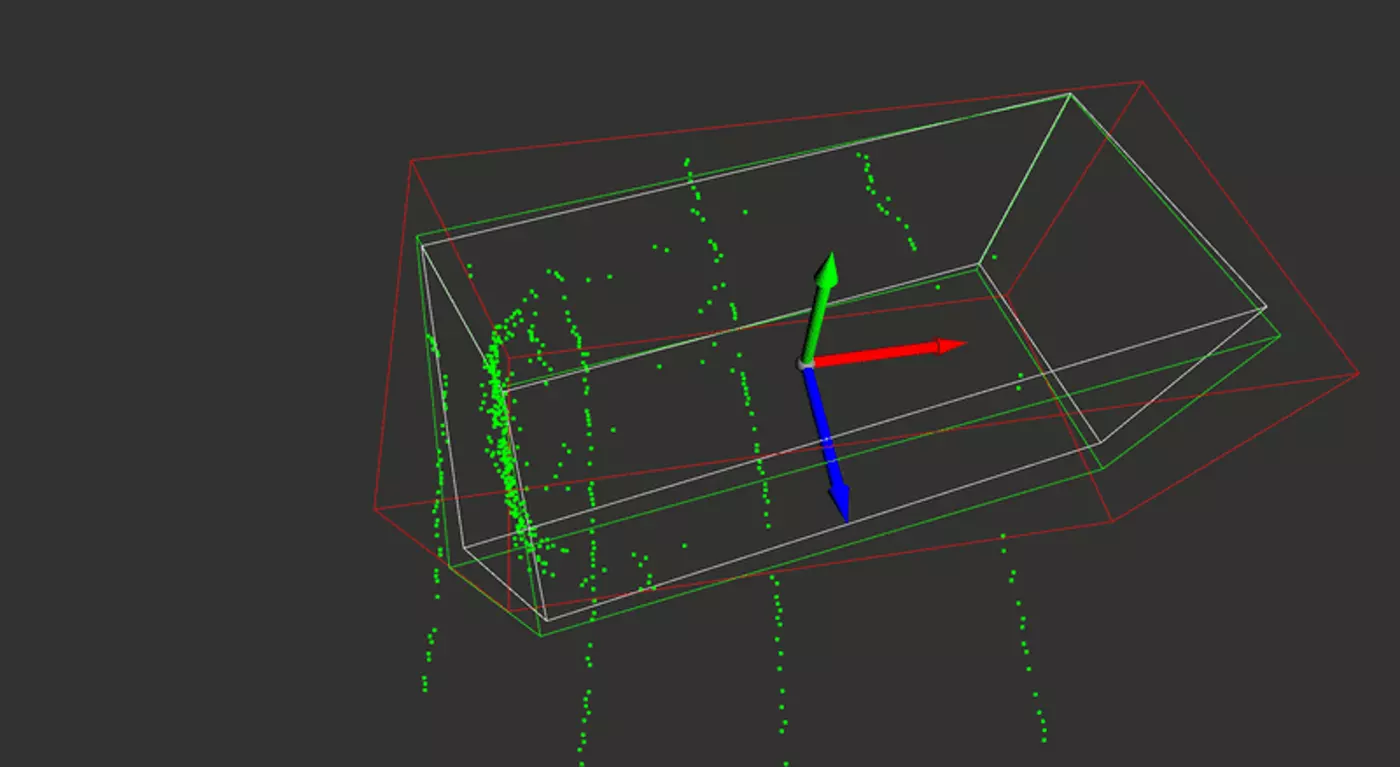
\includegraphics[scale=0.3]{3D_lidar_scanan.png}
        \caption{Contoh hasil bacaan \lidar\ 3D\cite{bs7}.}
        % https://understand.ai/blog/annotation/machine-learning/autonomous-driving/2021/03/29/3D-vs-2D-sensor-data-for-machine-perception.html
        \label{fig:Ch02_3d_bacaan}
    \end{figure}

    

    Tidak seperti kamera, \lidar\ berfungsi secara independen dari pencahayaan sekitar sehingga dapat memperoleh hasil yang baik saat siang dan malam tanpa kehilangan performa akibat gangguan seperti bayangan, sinar matahari, atau silau cahaya lampu \cite{bs8}.
    \begin{figure}[H]
        \centering
        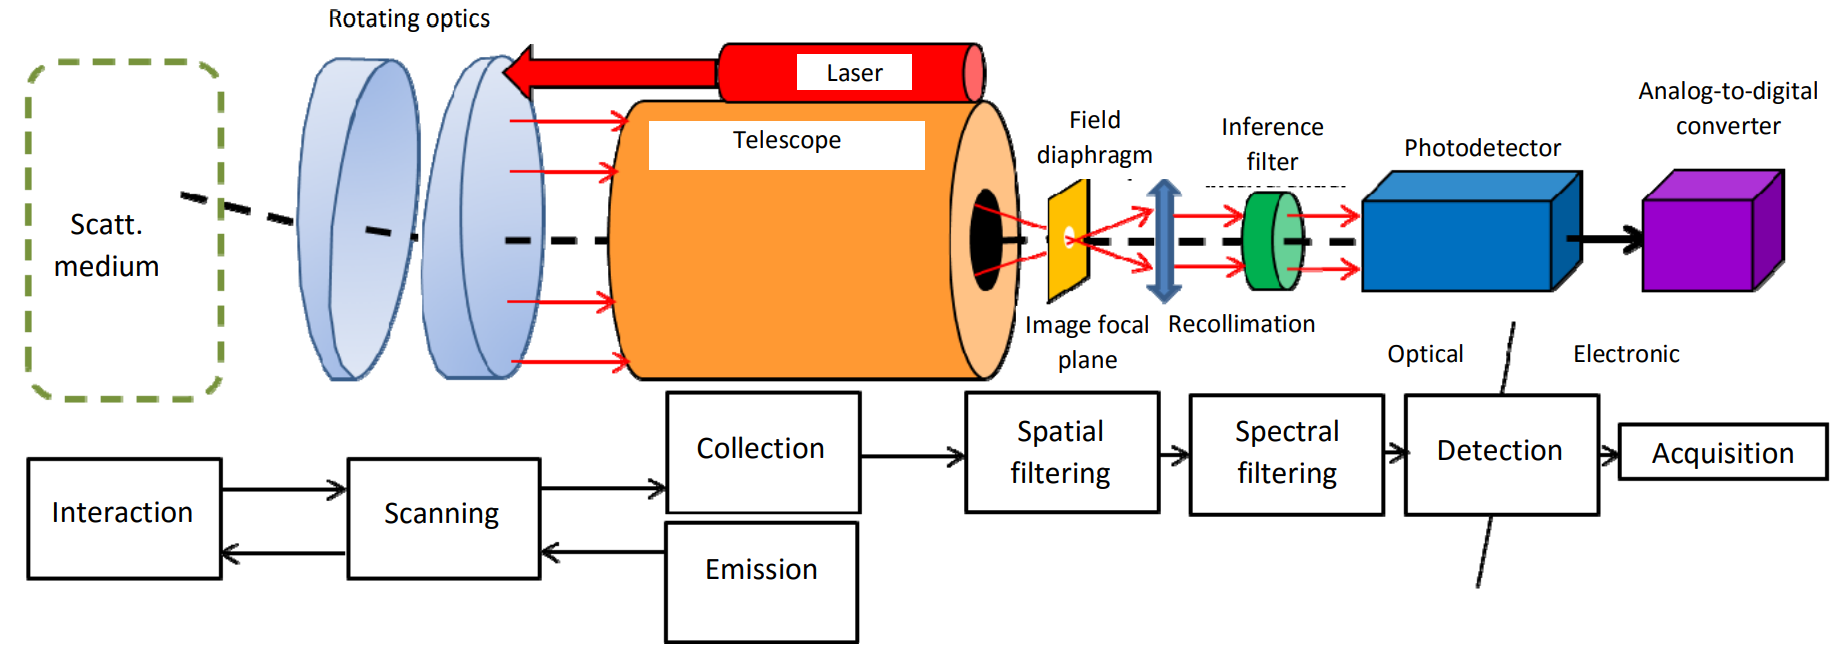
\includegraphics[width=\textwidth]{lidar_struktur.png}
        \caption{Gambar arsitektur \lidar\ Konvensional dan Fungsinya\cite{bs9}.}
        \label{fig:Ch02_lidar_struktur}
    \end{figure}
    % https://www.sciencedirect.com/science/article/pii/B9781785481024500053
    % See discussions, stats, and author profiles for this publication at: https://www.researchgate.net/publication/308941555
    Gambar \ref*{fig:Ch02_lidar_struktur} menunjukkan elemen-elemen penyusun \lidar\ konvensional beserta diagram fungsinya.
    Pulsa dipancarkan oleh sumber laser untuk setiap pengukuran LiDAR. Sinar laser yang dibentuk (diperluas dan dikoleksi) kemudian melewati optik pemindaian dan bergerak menuju media hamburan yang ditargetkan. Sinar yang mencapai target kemudian dihamburkan kembali ke arah LiDAR. Fluks optik dikumpulkan oleh sistem pencitraan optik, sering kali berdimensi besar seperti teleskop. 
    % A pulse is emitted by the laser source for each LiDAR measurement. Once the laser beam has been shaped (expanded and collimated), it passes through scanning optics and travels through space toward the targeted scattering medium. Following its interaction with the target, an echo of this pulse is backscattered toward the LiDAR. The optical flux is collected by an optical imaging system, often of large dimensions, such as a telescope. 
    \textit{Stray flux} dipisahkan dari sinyal melalui penyaringan spasial pada bidang fokus gambar juga melalui penyaringan spektral. Proses pertama membatasi bidang pandang ke ruang yang dilalui oleh pulsa laser, sedangkan yang terakhir digunakan untuk mengurangi bandwidth spektral sistem optik di sekitar panjang gelombang yang dipancarkan. Pemilihan panjang gelombang mengharuskan sinar untuk dikoleksi (paralel) di hulu elemen optik penyaringan spektral. Pada akhir rantai optik, fotodetektor mengubah aliran foton yang terdeteksi menjadi sinyal listrik kemudian  didigitalkan sebelum perekaman dan pemrosesannya. Penjelasan lebih lengkap mengenai bagian-bagian \lidar\ akan dijelaskan pada subbab \ref*{subsec: emisi} hingga subbab \ref*{subsec: Detection}.
    % Stray flux is separated from the signal by means of spatial filtering in the image focal plane as well as spectral filtering. The former restricts the field of view to the space traveled by the laser pulse, whereas the latter is used to reduce the spectral bandwidth of the optical system around the emitted wavelength. Note that wavelength selection requires the beam to be collimated (parallel) upstream of the spectral filtering optical element. At the end of the optical chain, a photodetector converts the detected photon flow into an electrical signal, which is in turn digitized prior to its recording and processing.
    \subsubsection{Emisi \lidar}
    \label{subsec: emisi}
    Transmisi berasal dari sumber pulsa laser yang memancarkan inframerah dekat (panjang gelombang 780-3.000 nm), terlihat (390-780 nm) atau domain ultraviolet (200-390 nm). Berbagai macam sumber laser dipasang di sekitar media penguat yang dapat berupa sel gas, kristal, dioda atau serat. Pemilihan panjang gelombang yang dipancarkan untuk aplikasi kehutanan dikondisikan berdasarkan transmisi atmosfer dan reflektansi vegetasi. Persyaratan lain dalam hal kekompakan, stabilitas, dan energi yang dipancarkan juga harus dipertimbangkan terutama dalam kasus durasi pulsa dari urutan beberapa nanodetik (diperlukan dalam kasus resolusi vertikal lebih rendah dari 1 m) dan frekuensi pengulangan yang tinggi.
    % The transmission is derived from a pulsed laser source emitting in the near-infrared (IR, wavelength 780-3,000 nm), visible (390-780 nm) or near- ultraviolet domain (UV, 200-390 nm). A wide variety of laser sources are built around amplifying media which can be gas cells, crystals, diodes or fibers. In the case of space or airborne LiDARs for forestry applications, the selection of the emitted wavelength is conditioned by atmospheric transmission and vegetation reflectance. Other requirements in terms of compactness, stability and emitted energy must also be taken into  consideration, especially in the case of pulse durations of the order of a few nanoseconds (required in the case of a vertical resolution lower than 1 m), and high repetition frequency. These various constraints restrict the selection to a range of basic sources summarized in Table 5.3. The table is ordered by the type of solid amplifying medium used.
    Dioda laser merupakan sumber laser yang paling kuat dan kompak yang dapat ditemukan dalam mode pulsa di dekat media IR. Panjang gelombang yang paling umum digunakan dan menguntungkan dalam hal energi adalah 905 nm. Dioda ini telah menjadi fitur jangkauan laser dan kontrol kecepatan pada \lidar, namun energi terbatas dioda membuat jangkauan LiDAR terbatas hingga beberapa ratus meter saja.
    % Laser diodes, the most robust and compact laser sources, may be found in pulsed mode in the near IR medium. The most commonly used and favorable wavelength in terms of energy is 905 nm. These diodes have become a feature of laser range-finders and speed control LiDARs. However, their energy remains limited (a few microjoules), which restricts the range of the LiDAR to a few hundred meters. Also in the near IR domain, fiber lasers at 1,064 nm (ytterbium) and 1,550 nm (erbium) are sufficiently compact and emit energy pulses of a few hundred microjoules.

    % 5.3.2.2. Transmitted beam shaping
    Sinar pada output laser biasanya harus sedikit menyebar dan diameternya meningkat untuk memenuhi kriteria yang berkaitan dengan keamanan mata. Divergensi sinar juga disesuaikan sesuai metode pengukuran yang dipilih, misalnya jejak kecil ( cm) dalam kasus gema diskrit \lidar\ atau pemindaian \lidar\ atau jejak besar dalam kasus \lidar\ gelombang penuh. Terdapat sistem optik \textit{afocal} yang melakukan pembentukan sinar terdiri dari dua lensa atau cermin yang menggabungkan titik fokus sedemikinan sehingga pembesaran yang dihasilkan lebih tinggi dari 1, seperti yang ditunjukkan pada Gambar \ref*{fig:Ch02_lidar_emisi}.
    \begin{figure}[H]
        \centering
        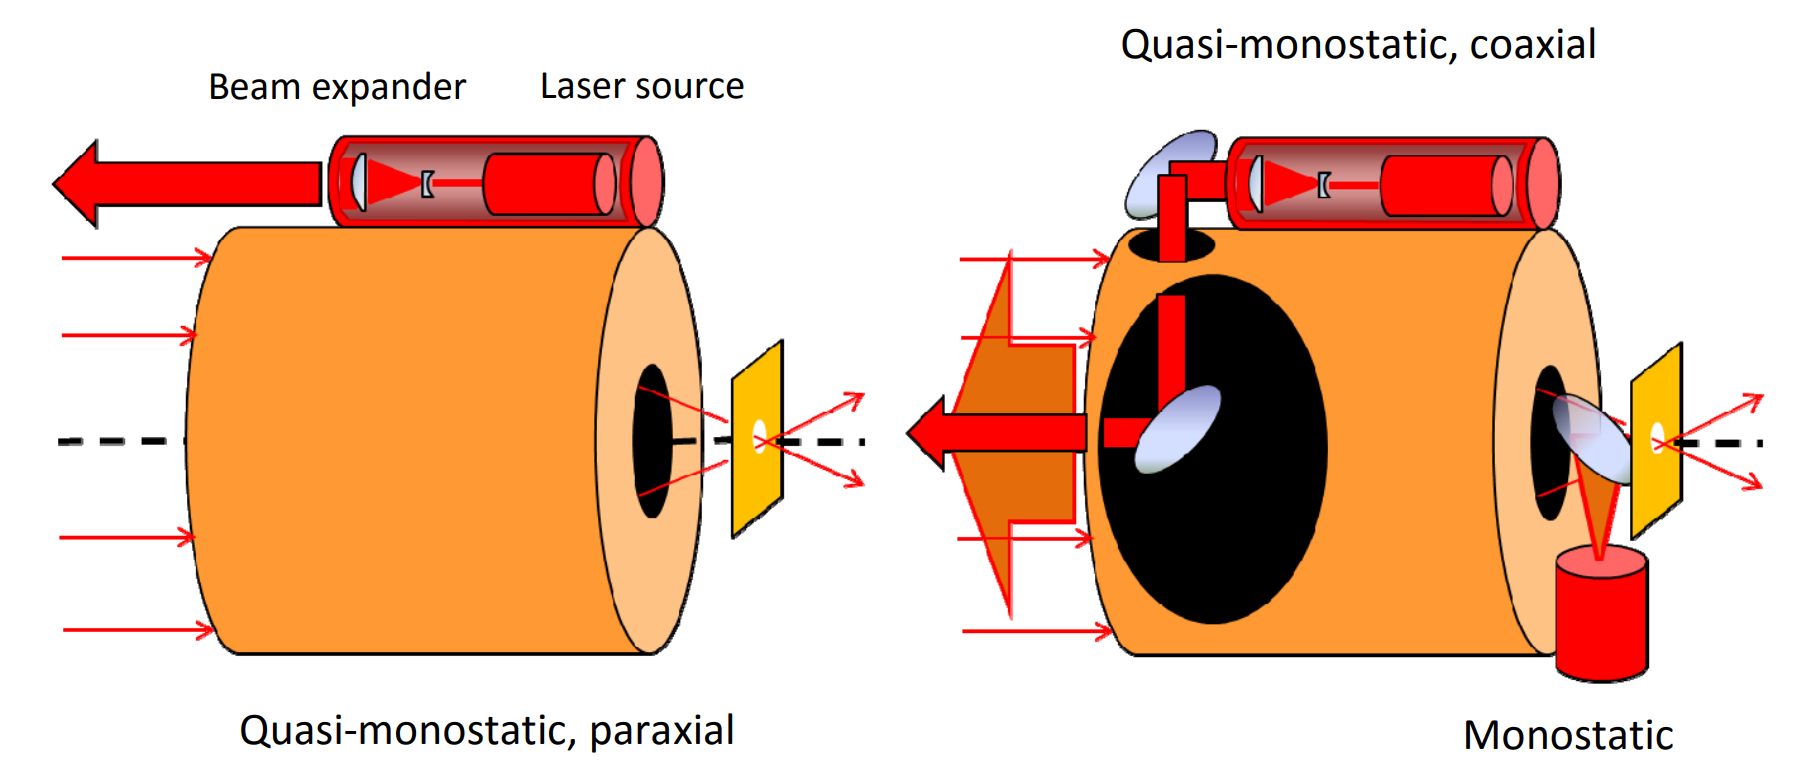
\includegraphics[width=0.7\textwidth]{emisi_lidar.png}
        \caption{Contoh Konfigurasi Emisi \lidar\cite{bs9}.}
        \label{fig:Ch02_lidar_emisi}
    \end{figure}
    
    Konfigurasi \lidar\ ditentukan oleh tata letak jalur pemancar dan penerimaan seperti yang disajikan pada Gambar \ref*{fig:Ch02_lidar_emisi}. Kedua komponen sistem optronik jika memiliki sumbu optik yang sama maka sistem tersebut dinamakan sebagai \textit{“monostatic”} sedangkan jika sumbu berbeda dan terpisah secara spasial maka disebut sebagai \textit{“bistatic”}. Konfigurasi terakhir juga memfasilitasi lewatnya jalur pemancar dan penerimaan melalui optik pemindaian yang sama.
    
    % A LiDAR configuration is determined by the layout of the emitting and receiving paths, as presented in Figure 5.4. If the two components of an optronic system have the same optical axis, said system is referred to as “monostatic”, whereas if the axes are distinct and spatially separated, it is referred to as “bistatic”. In our case, the proximity between the emitter and the receiver results in the LiDAR sensor being referred to as a “quasimonostatic” system, which represents an intermediate case. Systems in surface applications can adopt the so-called paraxial configuration, shown on the right. Nevertheless, in order to allow the overlap of emission and reception over a greater distance, a coaxial or fully monostatic configuration can be preferred, shown on the left. The latter configuration also facilitates the passage of the emitting and receiving paths through the same scanning optics.
% At the laser output, the beam usually has to be slightly divergent and its diameter increased, in order to meet the criteria pertaining to eye safety. If the laser beam is not eye-safe at emission, the aim is to reduce the nominal ocular hazard distance (NOHD) below the flight altitude or values provided by aviation specifications (a few hundred meters). Beam divergence is also adjusted as a function of the measuring method selected: a small footprint (~cm) in the case of a discrete echo LiDAR or a scanning LiDAR, or a large footprint in the case of a full waveform LiDAR. An afocal optical system carries out the beam shaping. It is made up of two lenses or mirrors having merged focal points and a resulting magnification higher than 1, as shown in Figure 5.4.

\subsubsection{Pemindaian}
\label{subsec: Scanning}
    \begin{figure}[H]
        \centering
        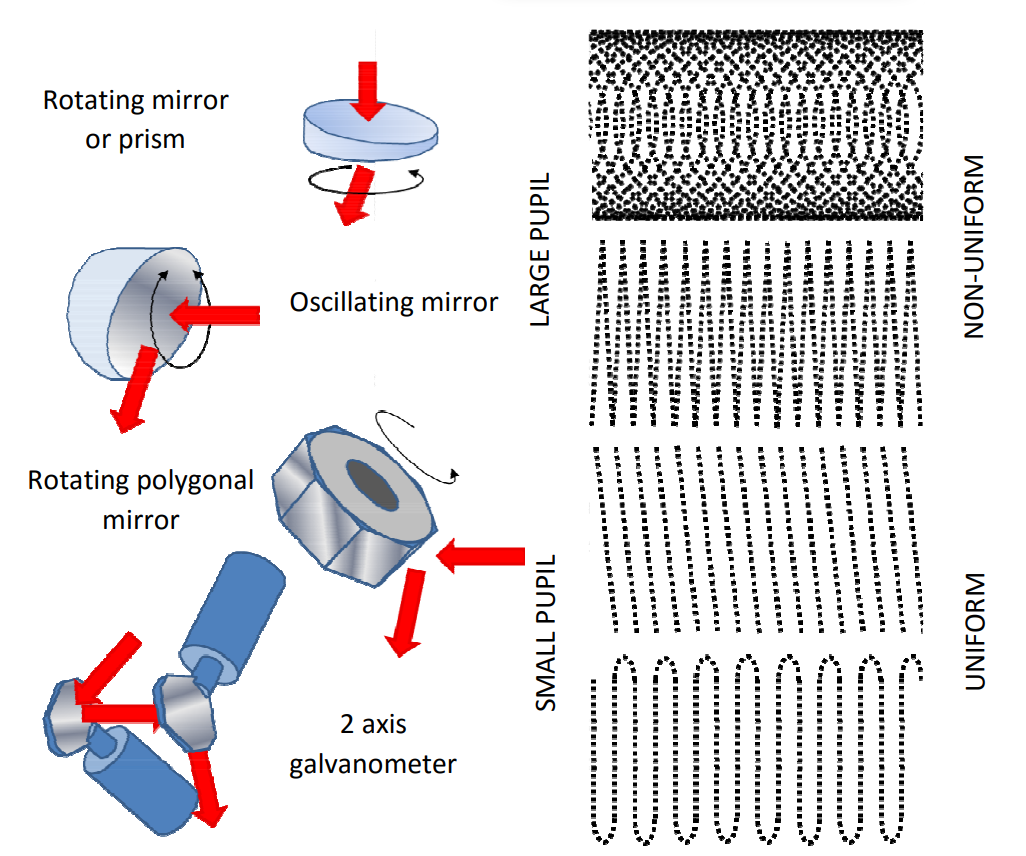
\includegraphics[scale=0.3]{pemindaian_lidar.png}
        \caption{Jenis-jenis Alat Pemindaian \lidar\ dan Pola Pemindaiannya\cite{bs9}.}
        \label{fig:Ch02_pemindaian_lidar}
    \end{figure}

    Berbagai elemen optik digunakan untuk menerapkan sistem \lidar\ yang mampu dengan cepat mengambil sampel pada permukaan besar. Empat solusi beserta pola pemindaian yang dihasilkan diilustrasikan pada Gambar \ref*{fig:Ch02_pemindaian_lidar}. Terlihat bahwa posisi berurutan jejak kaki laser pada jalur ini dikondisikan oleh frekuensi pengulangan pulsa. Pola-pola ini memiliki arti bahwa pengambilan sampel yang didistribusikan secara seragam tidak dapat dicapai dengan menggunakan optik berputar biasa. 
    Masalah lainnya yang terkait dengan implementasi sistem pemindaian adalah bahwa elemen terakhir harus mengakomodasi jalur pemancar dan penerimaan dengan minimal \textit{cross-talk}. Namun, sistem tercepat yang mampu menyediakan pemindaian seragam harus memiliki pupil kecil. Hal ini mengurangi dimensi sensor dan juga membatasi tingkat daya yang diterima.
% Various mobile optical elements may be used in order to implement an airborne scanning LiDAR system capable of quickly sampling large surfaces. Four such solutions are illustrated in Figure 5.5, along with the associated scanning patterns. It is clear that the consecutive positions of laser footprints on these paths are conditioned by the pulse repetition frequency (see section 5.3.2.1). It can still be inferred from these patterns that a uniformly distributed sampling cannot be achieved using basic rotating optics. Another severe constraint associated with the implementation of a scanning system is that the latter has to accommodate both emitting and receiving paths, with a minimum of cross-talk. However, the fastest systems capable of providing uniform scanning have small pupils. This imposes reduced sensor dimensions and therefore restricts the levels of power received.

\subsubsection{Penerimaan Fluks}
\label{subsec: receiving}

Berbagai macam sistem optik untuk menerima \textit{backscattered flux} dikembangkan sesuai dengan aplikasinya. Contoh lensa optik yang digunakan untuk menerima fluks yaitu:
\begin{enumerate}
    \item  Sistem \textit{catoptric} dan \textit{catadioptric}, termasuk cermin dan lebih sering disebut sebagai teleskop reflektif. Sistem ini berdiameter besar dan tidak mengalami aberasi kromatik yang mengurangi resolusi ketika pengamatan dilakukan pada spektrum yang luas. 
    % catoptric and catadioptric systems include mirrors and are more commonly referred to as reflective telescopes. These are large diameter systems that do not suffer from chromatic aberration, which reduces resolution when observations are conducted over a wide spectrum. 
    \item Sistem dioptrik (teleskop bias atau refraktor), hanya terdiri dari lensa dan jarang memiliki diameter yang sama dengan teleskop reflektif tanpa biaya tambahan atau berat dan dimensi keseluruhan yang kecil. Pada kasus \lidar\ monokromatik dan nilai diameter yang wajar, sistem ini masih dapat memberikan peningkatan kekompakan dan \textit{throughput}. Keuntungan utama sistem ini adalah stabilitasnya yang tinggi terhadap getaran yang memfasilitasi implementasinya pada \textit{platform} udara.
    % dioptric systems (refractive telescopes or refractors), solely made up of lenses, can rarely have the same diameter as reflective telescopes without additional costs or an inadmissible weight and overall dimensions. In the case of monochromatic LiDARs and reasonable diameter values, these systems can still provide improved compactness and throughput. Another major advantage is their high stability against vibrations, which facilitates their implementation on an airborne platform.
\end{enumerate}

Setelah fluks cahaya dikumpulkan, fluks dapat disuntikkan ke dalam serat optik yang ditempatkan di titik fokus sistem penerimaan untuk memisahkan deteksi dari kepala optik \lidar. Hal ini juga memungkinkan untuk membatasi obstruksi teleskop dengan menempatkan serat pada fokus cermin utama atau menggabungkan aliran beberapa teleskop sehingga menghasilkan pengurangan biaya dibandingkan dengan menggunakan satu teleskop besar. Serat optik terdiri dari inti dan dilapisi silika dengan indeks bias yang sedikit berbeda yang memungkinkan lewatnya cahaya. Diameternya harus dibatasi menjadi beberapa ratus mikron untuk menjaga fleksibilitas.
% Once the light flux has been collected, it can be injected into an optical fiber placed in the focal point of the reception system in order to dissociate the detection from the optical head of the LiDAR. This also makes it possible to limit telescope obstruction by placing the fiber at the focus of the primary mirror, or to combine the flow of several telescopes, a solution which results in reduced costs compared to a single larger telescope. An optical fiber is made up of a core and clad made of silica with slightly different refractive indices, which allows the assembly to guide light. Its diameter is limited to a few hundred microns in order to maintain flexibility.
% If used, it becomes the field diaphragm of the reception system, and reduces the field of view of the LiDAR to a great extent. The field of view can be expanded by using a bundle of fibers and a field lens, but this generates insertion losses which can amount to up to 60% of the incident light. 
% In the case of a good quality optical system, well adjusted in terms of focal length, the only dimensioning parameters of the receiver are its field of view and its effective area Aer which is connected to its actual area A and expressed as:

\subsubsection{\textit{Filtering}}
\label{subsec: Filtering}
Tingginya luminans lingkungan pada siang hari disebabkan ultraviolet atau inframerah menyebabkan perlunya untuk menyaring fluks cahaya yang masuk baik secara spasial maupun spektral. Proses ini diilustrasikan pada Gambar \ref*{fig:Ch02_filter_lidar}. Gambar menunjukkan proses penyaringan fluks yang datang untuk bidang fokus dan pupil.
\begin{figure}[H]
    \centering
    \begin{subfigure}[b]{.40\textwidth}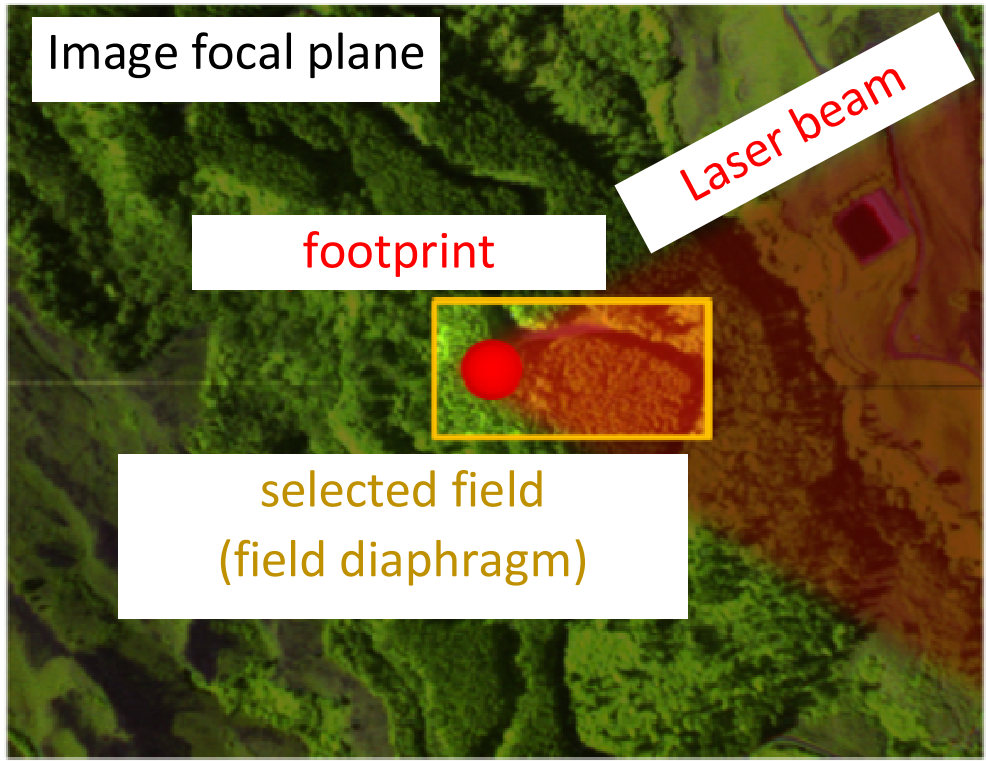
\includegraphics[width=\linewidth]{lidar_filtering.png}\caption{\textit{Spatial Filtering}}\label{Fig:Ch02_lidar_filtering1}\end{subfigure}
    \begin{subfigure}[b]{.40\textwidth}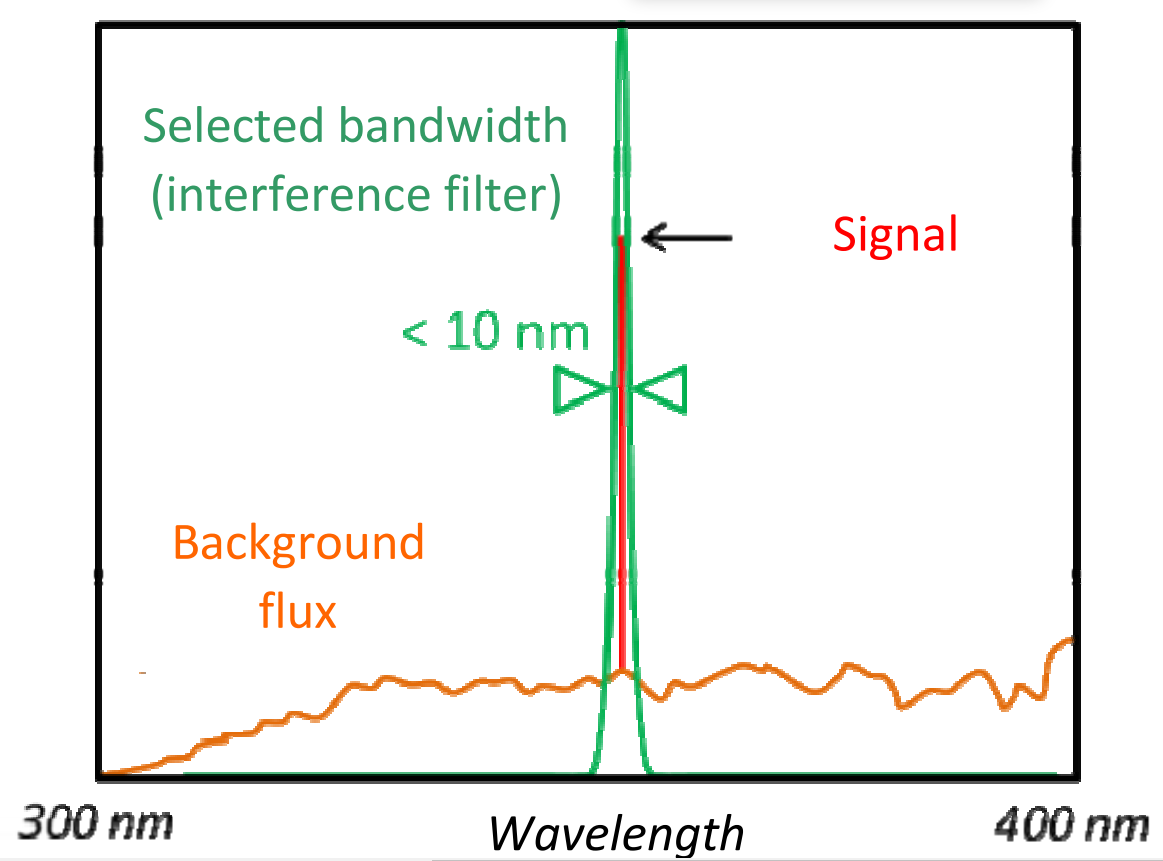
\includegraphics[width=\linewidth]{lidar_filtering2.png}\caption{\textit{Spectral Filtering}}\label{Fig:Ch02_lidar_filtering2}\end{subfigure}
    \caption{Proses Penyaringan Fluks Cahaya pada \lidar\cite{bs9}.}
    \label{fig:Ch02_filter_lidar}
\end{figure}
Pada bidang fokus gambar, diafragma lapangan membatasi bidang pandang sistem secara tepat ke ruang yang dilalui oleh sinar laser. Diafragma medan yang optimal untuk kasus konfigurasi paraksial adalah persegi panjang seperti yang diwakili pada Gambar 5.6. Konsekuensi dari keterbatasan bidang ini adalah adanya jarak pengukuran yang minimum, dalam kasus konfigurasi non-monostatik maka sinar hanya dapat memasuki bidang secara progresif.
% Due to the high luminance of daytime environment from near-ultraviolet o near-infrared, it is necessary to filter the incoming light flux both in a spatial and a spectral manner. This process is illustrated in Figure 5.7. In the image focal plane, a field diaphragm restricts the field of view of the system precisely to the space traveled by the laser beam. The optimum field diaphragm is rectangular in the case of a paraxial configuration, as represented in Figure 5.6. A consequence of this limitation of the field is the existence of a minimum measurement distance, knowing that: - in the case of non-monostatic configurations, the beam can only enter the field in a progressive manner;
Pada bidang pupil (misalnya pada sinar yang dikoleksi ulang setelah fokus pertama), ditempatkan filter dengan kemampuan spektral yang tinggi dan berpusat pada panjang gelombang yang dipancarkan untuk secara signifikan mengurangi \textit{bandwidth} sistem \lidar. Lebar spektral emisi kurang dari nanometer kecuali dalam kasus dioda laser dengan filter interferensi yang ditandai dengan lebar mulai dari 0,5 hingga 10 nm dapat digunakan. Komponen optik semacam itu dibangun menggunakan tumpukan film tipis dari tipe Bragg dan Fabry–Pérot untuk memadamkan spektrum yang luas dan membiarkan melalui garis sempit. 
% In the pupil plane (for example, on a recollimated beam after the first focus), a filter with a great spectral finesse and centered at the emitted wavelength is placed, in order to significantly reduce the bandwidth of the LiDAR system. The spectral width of the emission being less than a nanometer except in the case of laser diodes, an interference filter characterized by a width ranging from 0.5 to 10 nm can be used. Such an optical component is built using thin film stacks of the Bragg and Fabry–Pérot type in order to quench a broad spectrum and let through a narrow line. 

\subsubsection{Konversi Fluks ke Tegangan}
\label{subsec: Detection}
Konversi sinyal fluks optik menjadi tegangan listrik yang dapat diukur dilakukan oleh fotodetektor dengan mengubah setiap foton menjadi fotoelektron (dengan probabilitas yang ditetapkan oleh efisiensi kuantumnya) yang dilepaskan dalam resistor beban. Detektor cepat dan sangat sensitif yang digunakan dalam \lidar\ menyediakan sejumlah besar fotoelektron (antara 10 dan 10.000) untuk setiap foton insiden melalui fenomena penguatan internal. Kedua jenis detektor ini memiliki karakteristik yang sangat berbeda dalam hal sensitivitas, \textit{noise}, atau kapasitas listrik. Berbagai fenomena ini memiliki dampak signifikan pada \textit{link budget}, khususnya sebagai fungsi dari panjang gelombang yang dipilih untuk \lidar. 
% The conversion of the optical flux signal into measurable electric voltage is performed by a photodetector, which transforms each photon into a photoelectron (with a probability fixed by its quantum efficiency) discharged in a load resistor. The fast and highly sensitive detectors used in LiDAR, whether avalanche photodiodes (near IR) or photomultipliers (visible and UV), provide a large number of photoelectrons (between 10 and 10,000) for each incident photon via an internal gain phenomenon. Nevertheless, these two types of detectors have very different characteristics in terms of sensitivity, noise or electrical capacity (the latter restricting temporal resolution). These various phenomena have a significant impact on the link budget, in particular as a function of the wavelength selected for the LiDAR. The electronic detection configurations and the spectral ranges of various LiDAR detectors are illustrated in Figure 5.8. Table 5.5 presents the characteristics of these various internal gain photodetectors and more conventional photodiodes. They can be used in analog and photon counting mode.

% Robot Operating System
\section{Sistem Operasi Robot}
\label{sec:ROS} 

    Berbagai sistem operasi untuk robot saat ini telah dikembangkan. Sistem-sistem ini dapat digunakan untuk memprogram dan menyimulasikan robot dengan lebih mudah.
    Sebelum ada pengembangan sistem operasi robot, setiap \dev\ membuat program dari awal yang biasanya tidak bisa langsung diaplikasikan dan dikembangkan ke dalam robot lain.
    Berbagai sistem operasi dan program muncul untuk menjadi platform umum pada pengembangan aplikasi robotika. Berbagai sistem dapat digunakan untuk tujuan komersial maupun penelitian secara gratis dan \textit{open source}. Adanya algoritma siap pakai yang sudah tersedia dan dukungan komunitas yang besar membuat pengembangannya lebih mudah.
    
    \textit{Robot Operating System} (ROS) merupakan salah satu perangkat lunak khusus pengembangan robot yang bersifat \textit{open source} dengan \textit{libraries} dan \textit{tools} yang sudah tersedia untuk membangun program pada robot. ROS memiliki fitur yang banyak. Biasanya \dev\ menggunakan ROS untuk membuat prototipe, ROS tidak digunakan untuk membuat produk sebenarnya dikarenakan berbagai alasan seperti keamanan dan kekurangan pada pemrosesan \textit{real-time}\cite{br1}. Beberapa fitur ROS yang mendukung pengembangan robot antara lain yaitu:
    \begin{itemize}
     \item ROS menyediakan antarmuka penyampaian pesan untuk komunikasi antara dua program atau proses.
     \item ROS bukanlah sistem operasi yang sebenarnya tetapi merupakan sistem operasi meta yang menyediakan beberapa fungsi dan fitur mirip sistem operasi asli.
     \item ROS Mendukung bahasa pemrograman tingkat tinggi dan berbagai \textit{tools}.
     \item Kerangka kerja ROS terintegrasi dengan berbagai \textit{libraries} yang populer seperti OpenCV dan PCL.
     \item Algoritma siap pakai.
     \item ROS mudah digunakan untuk pembuatan prototipe.
     \item Komunitas pengembang yang banyak.
     \item \textit{Tools} dan simulator yang luas.
     \end{itemize}
% Why use ros?
% This is common question that developers ask when looking for a platform to program ROS. Although ROS has many features, there are still areas in which ROS can’t be used or is not recommended to use. In the case of a self-driving car, for example, we can use ROS to make a prototype, but developers do not recommend ROS to make the actual product. This is due to various issues, such as security, real-time processing, and so forth. ROS may not be a good fit in some areas, but in other areas, ROS is an absolute fit. In corporate robotics research centers and at universities, ROS is an ideal choice for prototyping. And ROS is used in some robotics products after lot of fine-tuning (but not self-driving cars).
% There was active development in robotics before the ROS project, but there was no common platform and community for developing robotics applications. Each developer created software for their own robot, which in most cases, couldn’t be reused for any other robot. Developers had to rewrite code from scratch for each robot, which takes a lot of time. Also, 
% most of the code was not actively maintained, so there was no support for 
% the software. Also, developers needed to implement standard algorithms 
% on their own, which took more time to prototype the robot.
% After the ROS project, things changed. Now there is a common platform for developing robotics applications. It is free and open source for commercial and research purposes. Off-the-shelf algorithms are readily available, so there is no longer a need to code. There is big community support, which makes development easier. In short, the ROS project changed the face of robotics programming.

\section{\textit{Object Recognition}}
\label{sec:object_detection} 

\textit{Object recognition} adalah bentuk aplikasi dasar untuk pemrosesan gambar dan visualisasi pada komputer. Istilah ini digunakan dalam berbagai aplikasi dan algoritma. Secara umum \objd\ bertujuan untuk mengingat data tentang penampilan objek tertentu dan memeriksa untuk mengevaluasi objek tersebut jenis apa dan di mana letaknya. 

\begin{figure}[H]
            \centering
            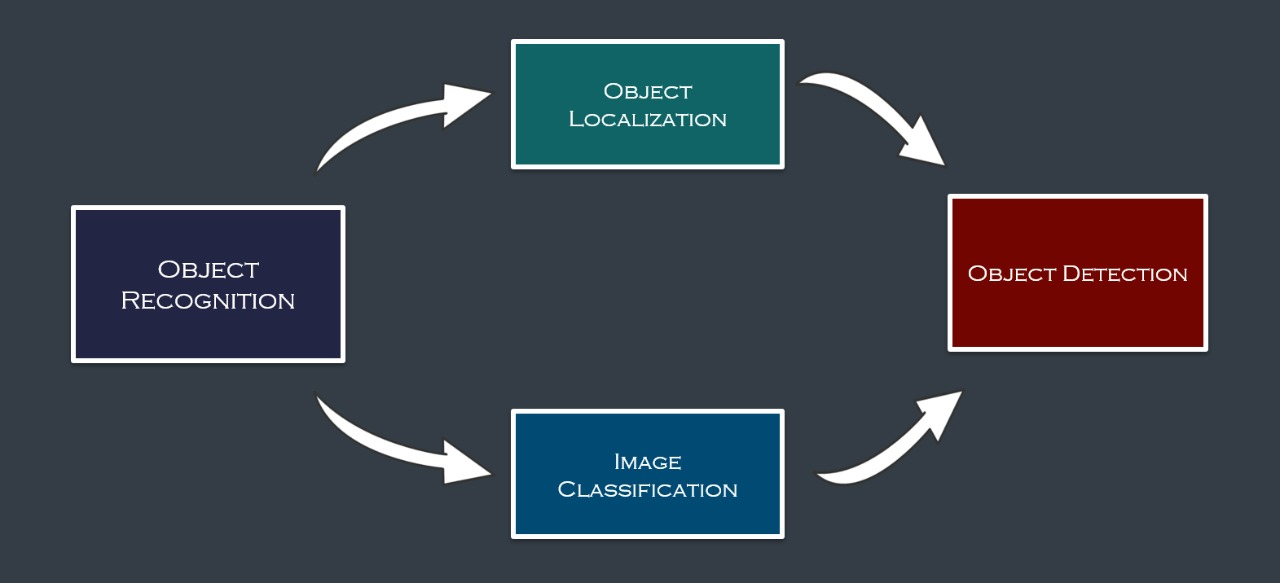
\includegraphics[scale=0.3]{Object_Rec.jpeg}
            \caption{Diagram Proses \textit{Object Recognition}.}
            \label{fig:Ch02_objectR}
        \end{figure}

Pada Gambar \ref{fig:Ch02_objectR} terlihat bahwa dalam object recognition terdapat dua proses terpisah yaitu \textit{object localization} dan \textit{image classification}. \textit{Object localization} merupakan komponen untuk menentukan posisi dan jarak benda atau objek yang terdeteksi di sekitar lingkungan. Image classification berfungsi untuk mengklasifikasi jenis objek yang terdeteksi. Kedua proses ini kemudian digabungkan menjadi \textit{object detection}. \textit{Object detection} biasanya menampilkan hasil klasifikasi dan letak objek hasil pemrosesan dalam \textit{bounding box} dengan keterangan nama objek. 

Ada banyak pendekatan yang berbeda untuk merancang \objd\, masing-masing memperhitungkan tuntutan spesifik dari konteks aplikasi yang diinginkan. Kategorisasi metode dan mode operasi dapat dikelompokkan melalui beberapa kriteria yang mengacu pada properti model data yang mewakili objek dan mode operasi skema \objd. Kriteria-kriteria tersebut adalah sebagai berikut\cite{br2}:
\begin{itemize}
\item Representasi objek yang diperoleh dengan mencari informasi tentang objek dapat diidentifikasi yaitu dengan geometri atau penampilan. Informasi geometris mengacu pada batas atau  bentuk permukaan objek. Sementara itu, model berbasis tampilan diturunkan dari karakteristik potret wilayah yang dicakup oleh objek.
\item Cakupan data objek yang dapat merujuk pada properti lokal objek (contoh: posisi sudut objek) atau karakteristik objek global (contoh: area, keliling, momen inersia).
\item Variasi objek yang dapat ditunjukkan oleh individu yang berbeda dari kelas objek yang sama.
\item Kualitas data gambar.
\item Strategi pencocokan untuk mengenali objek dalam gambar dilakukan di beberapa titik dalam aliran algoritma, misalnya pada model objek harus disejajarkan dengan konten gambar dengan cara kesamaan antara model dan gambar dimaksimalkan atau perbedaan diminimalkan.
\end{itemize}

%Sumber dari buku An Introduction to Object Recognition

% BAB 03 : Analisis Studi Pustaka Kunci dan Pemilihan Metode
\chapter{\uppercase{Analisis Studi Pustaka Kunci dan Pemilihan Metode}}
\label{chap:Analisis_Studi_Pustaka_Kunci_Pemilihan_Metode}
Deteksi manusia dan barang merupakan kemampuan yang sangat diperlukan di berbagai teknologi saat ini, tidak hanya robot. Hal ini dikarenakan banyaknya manfaat yang didapat dari pengembangannya untuk diaplikasikan menjadi fungsi lain. Berbagai metode dikembangkan untuk membangun sistem deteksi manusia dan barang. Bermacam-macam jenis sensor dilibatkan supaya dapat memberikan hasil yang bagus. Penggunaan \lidar\ untuk deteksi ini memberi keuntungan yaitu komputasi lebih rendah dengan akurasi sensor yang baik. Selain itu, pengguna tidak perlu memasangkan sensor pada target karena perangkat \lidar\ memancarkan pulsa sinar laser yang cepat dan mengukur jumlah waktu yang diperlukan untuk setiap pulsa yang memantul kembali untuk menentukan jarak target.

\section{Analisis Metode \textit{Leg Detection}}
\label{sec:Metode_02}

    Metode \textit{leg detection} (LD) mendeteksi manusia dengan melalui bagian kaki manusia sehingga \lidar\ diletakkan pada posisi yang cukup rendah yaitu $\pm 30$ cm sampai $50$ cm dari permukaan tanah untuk mendeteksi objek\cite{c1}. Metode ini sudah pernah dikembangkan pada ROS sehingga ROS sudah memiliki \textit{package} untuk LD, contohnya paket \textit{cob\_ people\_ perception} memungkinkan untuk menemukan pola berbentuk kaki dari pembacaan laser. Paket ini sayangnya sudah tidak dapat diakses lagi. Metode LD yang lainnya adalah metode pendeteksian kaki yang menggunakan beberapa sensor statis yang tersebar kemudian menggabungkannya dengan sistem jaringan dan server. Metode tersebut tidak dapat diterapkan pada proyek \capstone\ ini karena memerlukan sensor lebih dari satu dan sensor tidak bisa terpasang pada robot. Hal ini berarti metode pendeteksi kaki yang dapat diaplikasikan dan dikembangkan pada proyek ini adalah metode yang menggunakan sebuah sensor yang diletakkan pada robot. 

    Contoh metode LD dengan sensor pada robot yang telah berhasil dikembangkan adalah \textit{PeTra} yang dibuat oleh klub robotika \textit{University of León}. Sistem ini menggunakan pesan masukkan dari pemindai \lidar\ dan menggunakan data terlatih untuk mengklasifikasikan kelompok yang dideteksi termasuk kaki atau bukan. Deteksi dilakukan oleh \textit{classifier} menggunakan algoritma \textit{Random Trees} yang diimplementasikan dengan API OpenCV. \textit{Training data} diperoleh dengan mengumpulkan data dari satu orang yang berjalan dalam garis lurus menuju robot dan kemudian berbalik untuk menjauhi robot yang berada dalam kondisi tetap diam. Proyek ini belum menerima pengembangan berkelanjutan dan tidak ada versi perangkat lunak untuk versi ROS terbaru. 

    Metode lain pengembangan LD yang saat ini banyak dilakukan adalah dengan sensor berada di robot untuk mendeteksi bentuk geometri kaki manusia. Metode ini dikembangkan untuk mendeteksi banyak manusia berjalan dari suatu robot bergerak. Biasanya metode ini dikembangkan untuk melacak orang-orang yang hanya mengenakan celana agar bentuk geometris kaki lebih mudah dibedakan dari objek lain.
    % Penggunaan karakteristik geometris kaki manusia dan frekuensi-fase gerakan berjalan telah diuji (Lee et al., 2006), tetapi tidak dapat menangani oklusi parsial, perubahan kecepatan orang, dsb. Sensor akan memindai seluruh objek sehingga benda-benda seperti meja atau kaki kursi, batang tanaman, dll., mungkin mudah dikacaukan dengan kaki orang. Juga sulit untuk melacak orang tertentu (sepasang kaki) di lingkungan yang ramai karena banyak tabrakan dapat terjadi.
    Kesulitan utamanya berasal dari \textit{uncertainty} dan \textit{noise} data sensor karena objek yang dilacak dan juga sensor pada robot akan bergerak dalam aplikasi situasi nyata. Selain itu, terjadi beberapa oklusi yang terjadi saat pemindaian objek lain, selain itu kadang-kadang salah satu dari dua kaki tidak dapat dideteksi sesuai dengan arah gerakan berjalan manusia. Solusi untuk mengatasi masalah tersebut yaitu dengan menggunakan Extended Kalman Filter untuk memodelkan manusia yang berjalan.
    %
    % They used multiple static LRF sensors
    % attached on the ground and combined them with network and
    % server system. The method is extended for using both LRF
    % and vision[8,10].
    %
    % Different solutions have been proposed previously in the literature to deal with the problem of tracking people using a 2D LIDAR scanner mounted on a mobile robot. Navigation in peopled, mapped, indoor environments has been recently reviewed (Rios-Martinez et al., 2015). 
    %
    % The use of the geometric characteristics of human legs and the frequency and phase of walking motion have been tested (Lee et al., 2006), but cannot deal with partial occlusions, changes in peoples' speed, etc. In this article we are concerned with the specific problem of detecting pairs of legs (from a person) and being able to track them.
    %
    % The charm point of the approach of this paper is to track multiple walking humans from a ``moving'' robot with walking model. Its principal difficulties come from the uncertainty and noise of sensor data, because not only the object being tracked but also the sensor on a robot is moving in real applications. Moreover, there happen some occlusions owing to screening by another object, and sometimes one of two legs cannot be detected according to the direction of human walking motion. These also increase the uncertainty of extracted human data. To cope with those difficulties, human walking model with Extended Kalman Filter is utilized.
    % Tracking procedure is designed as following sequences that are iterated every scanning time. In this research, it is assumed that we track people putting on just general trousers, excepting skirt or other dressing style, and the knee part of human leg is scanned.:
    Prosedur \textit{tracking} ini dirancang dari beberapa tahap yang terus diulang-ulang setiap pemindaian. Berikut adalah langkah-langkah yang ditempuh untuk metode LD dengan sensor pada robot\cite{c1b}:
    \begin{enumerate}
        \item Pengelompokan Data: Hal ini diperlukan untuk mengekstrak data orang berjalan dari data pemindaian sensor yang berupa data mentah dengan informasi baik dari orang-orang maupun lingkungan. Data hasil pemindaian dibagi menjadi beberapa cluster dan cluster yang ukurannya mirip kaki manusia (lebar kurang dari 25 cm) diklasifikasikan menjadi kandidat kaki.
        % Data Clustering: Firstly, it is needed to extract the data of walking people from the scanning data from LRF sensor because raw data has information of both people and environments. 

        \begin{figure}[H]
            \centering
            \begin{subfigure}[b]{.30\textwidth}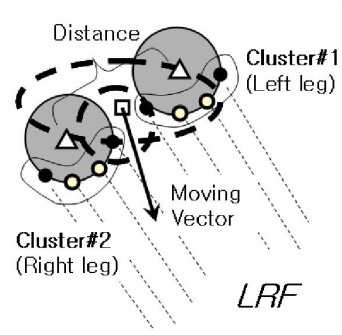
\includegraphics[width=\linewidth]{bab3/leg_detection1.png}\caption{Dua Kaki Manusia}\label{Fig:Ch02_leg1}\end{subfigure}
            \begin{subfigure}[b]{.30\textwidth}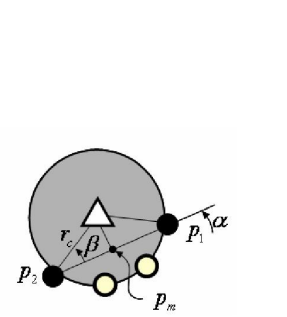
\includegraphics[width=\linewidth]{bab3/section_leg.png}\caption{Satu Kaki Manusia}\label{Fig:Ch02_leg2}\end{subfigure}
            \caption{Tampilan Data Kaki Manusia dari Atas\cite{c1b}.}
            \label{Fig:ch02_posisi_leg}
        \end{figure}
        \item Proses Menemukan Posisi Kaki: selanjutnya, posisi bagian tengah kaki harus dihitung karena kandidat kaki yang diberikan dari proses pengelompokan sebelumnya hanya memiliki bagian kaki seperti yang ditampilkan pada Gambar \ref{Fig:Ch02_leg1}. 
        % Finding Leg Position: Next, the center of leg section should be computed because leg candidate given from previous clustering process has just a part of leg section as displayed in Fig. 2 (a). 
        Gambar \ref{Fig:Ch02_leg2} menunjukkan satu lingkar kaki dimana lingkaran kecil menunjukkan titik-titik dipindai oleh sensor jarak dengan $p_1$ dan$p_2$ adalah titik awal dan akhir dari kandidat kaki. 
        Posisi tengah bagian kaki adalah dihitung dengan mempertimbangkan geometri kaki dengan persamaan berikut.
        \begin{equation}
            \begin{pmatrix}
                x_{leg}\\
                y_{leg}
            \end{pmatrix} =
            \begin{pmatrix}
                x_{p2}\\
                y_{p2}
            \end{pmatrix} +
            \begin{pmatrix}
                \glsadd{r_c}
                r_c\glsadd{r_c} \cos (\alpha + \beta)\\
                r_c\glsadd{r_c} \sin (\alpha + \beta)
            \end{pmatrix}
        \end{equation}
        dimana $p_1, p_2 $ dan $r_c\glsadd{r_c}$ menunjukkan titik pertama kaki, terakhir dari kaki, dan jari-jari kaki yang diasumsikan $\pm 7$ cm, kemudian dihitung titik tengah kaki $(x_{leg},y_{leg})$.

        \item Proses Menghubungkan Posisi Manusia dengan Kandidat Kaki: Kandidat kaki yang dibuat pada langkah pengelompokan sebelumnya digunakan sebagai posisi baru manusia berjalan, sehingga objek manusia dengan dua kaki yang dibuat pada pemindaian sebelumnya terhubung dengan kandidat kaki baru.
        % Connecting Human Objects to Leg Candidates: Leg candidates made in previous clustering step are used as the new position of walking human. Thus, human objects created in the past scanning time have two legs, and both of them are connected with new leg candidates. 
        \item Pembuatan Objek Manusia Baru: Objek manusia yang baru akan dibuat dari kandidat kaki lainnya yang tidak terhubung ke objek manusia yang ada dalam prosedur penghubungan sebelumnya. Sepasang kandidat kaki yang jaraknya di antara mereka lebih pendek dari langkah normal ($<50$ cm) menjadi objek manusia baru.
        % Creating New Human Object: New human object are created from the rest of leg candidates which are not connected to the existing human objects in the previous connecting procedure. A pair of leg candidates whose distance between them is shorter than that of normal stride(<50cm) becomes a new human object.
        \item \textit{Update} Objek Manusia: Keadaan objek manusia di-\textit{update} menggunakan model berjalan manusia dengan data posisi diberikan dari prosedur sebelumnya. Beberapa objek manusia tanpa data posisi baru dari waktu pemindaian ini juga diperbarui dengan prediksi. Kandidat kaki baru yang belum terhubung ke objek manusia sebagai data pemindaian baru, maka sementara waktu akan dikategorikan sebagai keadaan oklusi. Data tersebut akan dihilangkan jika waktu oklusi objek manusia melebihi nilai yang diberikan.
        % Update Human Objects: The states of human objects are updated using human walking model with the measured position data given from previous procedures. Some human objects without new position data from this scanning time are also updated with just prediction. If new leg candidate has not been connected to a human object as new scanning data for a while, it means occlusion state. If occlusion time of a human object exceeds a given value, we consider it as disappearance and delete it. And states of another objects created in this scanning time are initialized. Walking model used in this paper will be discussed in detail in the next chapter.
        \item Pemindaian Berikutnya: Setelah proses selesai, maka akan dilanjutkan proses pemindaian selanjutnya dengan data baru yang diterima sensor.
    \end{enumerate}

\section{Analisis Metode \textit{Torso Detection}}
\label{sec:Metode_03}

    % In supervised machine learning, a group of labelled samples is the training data with known category, and the model learns from the correctly identified samples. 

    Metode ini memanfaatkan bentuk \textit{elips} untuk melacak bagian dada manusia kemudian menentukan objek terdeteksi merupakan manusia atau bukan\cite{c2}. Dada memiliki bentuk yang lebih sederhana dan tidak banyak mengalami perubahan ketika aktivitas. Seperti pendeteksian pada umumnya, masalah pendeteksian ditangani dengan memanfaatkan algoritma klasifikasi. Pengamatan individu yang diubah menjadi properti yang dapat diukur dikenal sebagai fitur. Algoritma yang melakukan klasifikasi disebut pengklasifikasi/\textit{classifier}. Pemilihan \textit{classifier} merupakan bagian penting dalam proses deteksi.

    Langkah pertama dilakukan segmentasi data berdasarkan pada pendeteksian titik-titik diskontinuitas dalam pemindaian laser. Laser mencapai jangkauan dan arah $\{r_i, \theta\glsadd{theta}_i \}$ sejauh objek dalam bidang pandangnya dengan $i$ bernilai $i = 1......n.$. Segmentasi dilakukan dengan menggunakan teknik \textit{model based} yang direalisasikan menggunakan \textit{Extended Kalman Filter} (EKF) \cite{c4}, data dapat dipartisi menjadi segmen-segmen $S = \{s_1, s_2, ,...,s_M\}$ seperti pada Gambar \ref{fig:Ch03_segmentasi}.
        
        \begin{figure}[H]
            \centering
            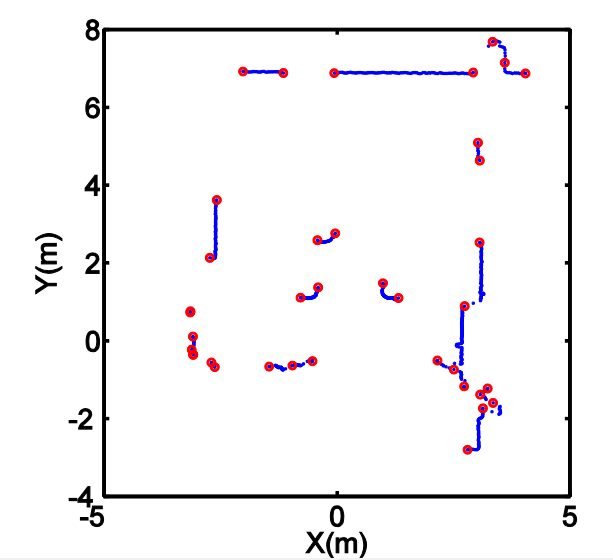
\includegraphics[scale=0.35]{segmentasi.png}
            \caption{\textit{Plotting} segmentasi bacaan \lidar\cite{c2}.}
            \label{fig:Ch03_segmentasi}
        \end{figure}

        Langkah selanjutnya setelah melakukan segmentasi adalah ekstraksi fitur-fitur yang akan digunakan dalam deteksi manusia. Fitur pertama adalah panjang segmen yang diperoleh dari persamaan berikut:
        \begin{equation}
            \sqrt{(x_n-x_1)^2+(y_n-y_1)^2}
        \end{equation} 
        dengan panjang segmen dihitung dari titik awal $(x_1,y_1)$ hingga titik $akhir (x_n,y_n)$. Fitur kedua yang dicari adalah rasio sumbu mayor dan minor elips. 
        \textit{Cross section} dada manusia umumnya dapat diperkirakan dengan elips. Oleh karena itu, algoritma elips diimplementasikan pada hasil segmentasi. Fitur ketiga yang dicari adalah \textit{mean} karakteristik kurva dari segmen. Nilai perkiraan kelengkungan diskrit dari kurva adalah\cite{c2b}:
        \begin{equation}
            k=\frac{4A}{d_1d_cd_n}
        \end{equation}
        dengan $d_1, d_c, d_n$ merupakan jarak antar titik $x_1, x_n, x_c\glsadd{x_c}$ yang diperoleh dari titik awal kurva, titik akhir kurva, dan titik tengah kurva, kemudian $A$ adalah area di dalam ketiga titik tersebut. 
        Fitur keempat adalah rasio jarak antara sumber laser menuju pusat segmentasi dari sekumpulan titik yang dihitung:
        \begin{equation}
            \sqrt{\frac{x_c\glsadd{x_c}^2+y_c\glsadd{y_c}^2}{n}}
        \end{equation} 
        
        dengan $(x_c\glsadd{x_c},y_c\glsadd{y_c})$ adalah pusat segmen dan $n$ adalah jumlah titik.

    Langkah selanjutnya adalah melakukan ekstraksi fitur yang berupa panjang segmen, rasio antara sumbu mayor dan sumbu minor elips, karakteristik kelengkungan segmen, dan jarak antara sumber laser dengan pusat segmen. Setelah itu dilakukan klasifikasi menggunakan \textit{Radial Basis Function Support Vector Machines} (RBFSVM) yang dituliskan menjadi fungsi kernel:
    \begin{equation}
        K(\mathbf{F_i,F_j})=exp(-\gamma||\mathbf{F_i}-\mathbf{F_j}||^2), \gamma >0,
    \end{equation}
    \begin{tabbing}
        dengan: \=\\
            \>$\mathbf{F_i}$ \qquad \=: \textit{training vectors i},\\ 
            \>$\mathbf{F_j}$ \>: \textit{training vectors j},\\
            \>$\gamma$ \>: parameter kernel.
    \end{tabbing}
    
\section{Analisis Metode \textit{Hip Detection}}
\label{sec:Metode_01}

    Metode ini menggunakan \lidar\ untuk membaca lingkungan dengan cara memancarkan pulsa sinar laser yang cepat, kemudian hasil bacaan \lidar\ perlu diubah ke dalam bentuk denah dua dimensi (2D). \lidar\ 2D lebih diutamakan untuk digunakan daripada \lidar\ 1D dan 3D untuk mencapai keseimbangan antara kompleksitas komputasi dan biaya rendah. Hasil bacaan mentah \lidar\ dikurangi jumlah dimensinya dengan ekstraksi. Kemudian pada fase tampilan, ditunjukkan berapa manusia yang terdeteksi pada denah output serta menghitung jumlahnya secara \textit{real-time}. Seperti yang terlihat pada Gambar \ref{fig:Ch02_Hip_Detec}, metode ini mengimplementasikan aplikasi untuk penghitungan dan pendeteksian orang dengan menempatkan LIDAR pada tingkat yang lebih tinggi (setinggi panggul)\cite{c3}. Target keluarannya yaitu membedakan manusia dari objek sekitarnya. 
    Fitur diperoleh dari data \lidar\ asli yang bertindak sebagai masukan untuk pelatihan atau prediksi model. Proses penurunan fitur dikenal sebagai ekstraksi fitur yang dilakukan untuk mengurangi jumlah dimensi. 
    
    \begin{figure}[H]
            \centering
            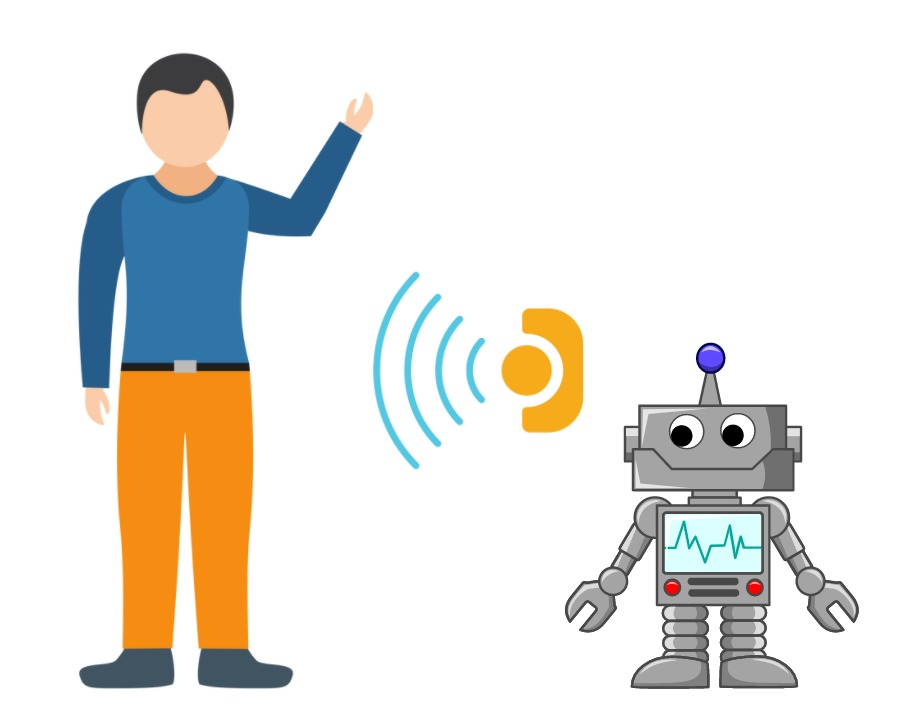
\includegraphics[scale=0.3]{Hip_detec.jpeg}
            \caption{Ilustrasi Metode \textit{Hip Detection}.}
            \label{fig:Ch02_Hip_Detec}
        \end{figure}
 
    Sebelum melakukan klasifikasi, data yang didapat perlu dikelompokkan. Teknik \textit{clustering} adalah teknik pengelompokan objek berdasarkan kesamaan karakteristiknya. Pengelompokan ini menggunakan metode Density-Based Spatial Clustering of Applications with Noise(DBSCAN). DBSCAN digunakan untuk mengelompokkan titik berdasarkan jarak menggunakan nilai  \textit{minimum points} (MinPts) dan epsilon ($\backepsilon$). $\backepsilon $ mendefinisikan radius lingkungan di sekitar titik $x$. MinPts adalah jumlah minimum tetangga dalam radius $\backepsilon$. Selanjutnya untuk memprediksi apakah \textit{cluster} termasuk manusia atau bukan manusia diperlukan algoritma klasifikasi yaitu menggunakan algoritma Random Forest. 
    
    Ukuran \textit{cluster}, perbedaan standar dari \textit{mean}, rata-rata perbedaan \textit{mean}, lebar, \textit{linearity}, \textit{circularity}, jari-jari, \textit{boundary regularity}, \textit{mean curvature},\textit{ angular difference, inscribed angular variance, standard inscribed angular variance}, jarak, dan jarak/ukuran \textit{cluster} adalah 14 fitur yang diekstraksi dari \textit{cluster}. Semua fitur ini diekstraksi dari setiap \textit{cluster} diperhitungkan untuk mengklasifikasikan sampel yang masuk.  Terakhir, pada fase tampilan ditunjukkan manusia yang terdeteksi serta menghitung secara \textit{real-time} melalui denah 2D dari data \lidar.

\section{Pemilihan Metode}
\label{sec:Pemilihan_Metode}

Pemilihan metode dapat menghasilkan hasil lebih maksimal
dengan memahami kelebihan dan kekurangan masing-masing metode. Berikut akan dibahas kelebihan dan kekurangan untuk masing-masing metode berdasarkan tabel kelebihan dan kekurangan masing-masing metode yang ditunjukkan pada Tabel \ref{tab:Ch05_Methods}.
\begin{longtable}{|c|L{1.8 cm}|L{4.8 cm}|L{4.8cm}|L{0.6cm}|}
   \caption{Kelebihan dan Kekurangan Metode-Metode Sistem Deteksi} 
   \label{tab:Ch05_Methods}
   \vspace{-0.75em}\\
   \hline
   \multicolumn{1}{|c|}{\textbf{No}} & \multicolumn{1}{|c|}{\textbf{Metode}}  & \multicolumn{1}{|c|}{\textbf{Kelebihan}} & \multicolumn{1}{|c|}{\textbf{Kekurangan}} & \multicolumn{1}{|c|}{\textbf{Total Skor}} \\ \hline
   1           & Leg Detection      &  \begin{tabular}[C{|c|}]{@{}L{4.5 cm}@{}}
       \begin{itemize}
           \item Sudah pernah dikembangkan pada ROS(+3).
           \item Letak \lidar\ rendah sehingga semua objek di sekitarnya dapat terbaca(+3).
       \end{itemize}
   \end{tabular}        & \begin{tabular}[C{|c|}]{@{}L{4.5 cm}@{}}
   \begin{itemize}
           \item \textit{Package} ROS sudah tidak dapat diakses dengan versi ROS terbaru(-2).
           \item algoritma lebih rumit ketika dikembangkan untuk \textit{tracking} jika jumlah kaki banyak(-1).
       \end{itemize}
   \end{tabular} 
   & \multicolumn{1}{|c|}{3}  \\ \hline
   2           & Torso Detection     & 
   \begin{tabular}[C{|c|}]{@{}L{4.5 cm}@{}}
       \begin{itemize}
           \item Bentuk torso tidak mengalami banyak perubahan dan banyak pergerakan(+2).
           \item Bentuk tidak serumit kaki manusia(+1).
       \end{itemize}
   \end{tabular}
   & \begin{tabular}[C{|c|}]{@{}L{4.5 cm}@{}}
       \begin{itemize}
           \item Pemasangan terlalu tinggi(-1).
           \item \textit{backscattering noise} yang diterima banyak karena \lidar\ dekat dengan sumber cahaya lainnya(-2).
       \end{itemize}
   \end{tabular}   
   & \multicolumn{1}{|c|}{0}  \\ \hline
   3           & Hip Detection & 
   \begin{tabular}[C{|c|}]{@{}L{4.5 cm}@{}}
       \begin{itemize}
           \item Bentuk sederhana(+2).
           \item Pemasangan \lidar\ tidak terlalu rendah atau tinggi(+2).
       \end{itemize}
   \end{tabular}        
   & \begin{tabular}[C{|c|}]{@{}L{4.5 cm}@{}}
       \begin{itemize}
           \item Sama dengan metode \textit{torso detection} namun dengan jumlah \textit{backscattering noise} lebih sedikit(-2).
       \end{itemize}
   \end{tabular} 
   & \multicolumn{1}{|c|}{2}  \\ \hline

\end{longtable}
    Pada Tabel \ref*{tab:Ch05_Methods} terlihat bahwa masing-masing metode memiliki skor untuk setiap poin kelebihan dan kekurangan. Terlihat antara metode-metode tersebut, nilai skor yang paling tinggi dimiliki metode LD. Penerapan metode ini memerlukan perancangan dari pemrosesan data mentah \lidar\ hingga pendeteksian. Bentuk geometri hasil pembacaan kaki manusia akan digunakan sebagai pembeda manusia dengan objek yang lainnya.
    
    Metode LD juga sesuai dengan rencana kondisi peletakan \lidar\ pada robot yaitu setinggi kaki. \lidar\ yang diletakkan pada posisi bawah robot akan lebih mudah memperoleh data data dibandingkan posisi peletakan yang lebih tinggi. Berbeda dengan metode awal \textit{hip detection}, metode ini lebih mudah diaplikasikan pada robot dikarenakan peletakan sensor dan proses pemindaian lingkungan tidak terganggu dengan bagian robot lainnya. Objek yang terdeteksi juga memiliki lebih sedikit variasi bentuk daripada objek-objek yang terbaca pada peletakan \lidar\ yang lebih tinggi.
    
    Oleh karena itu, metode yang digunakan adalah metode LD.
    Metode ini akan diimplementasikan secara sederhana yaitu dengan mendeteksi objek berupa lingkaran yang sesuai untuk mengidentifikasi kaki manusia. Objek-objek di sekitar akan dibedakan menjadi dua bentuk yaitu garis lurus dan lingkaran. Objek-objek lingkaran kemudian dikelompokkan yang memenuhi syarat sebagai kaki manusia lalu posisi manusia ditentukan dari kaki-kaki yang terdeteksi tersebut.


% Tracking peoples' legs using only information from a 2D LIDAR scanner in a mobile robot is a challenging problem because many legs can be present in an indoor environment, there are frequent occlusions and self-occlusions, many items in the environment such as table legs or columns could resemble legs as a result of the limited information provided by two-dimensional LIDAR usually mounted at knee height in mobile robots, etc. 

% for instance, the cob\_people\_perception package allows to find leg-like patterns of laser scanner readings. This software is based on the LD approach and implementation.\\
% It obtains incoming messages from the LIDAR scanner and uses trained data to classify the groups of laser records as possible legs. Detection is performed by a classifier using Random Trees implemented with the OpenCV API. However, LD has an important drawback; the project has not received continuous development and there is not a version of the software for the latest ROS versions.

% Metode ini menggunakan pesan masuk dari pemindai LIDAR dan menggunakan data terlatih untuk mengklasifikasikan kelompok termasuk kaki atau bukan. Deteksi dilakukan oleh \textit{classifier} menggunakan \textit{Random Trees} yang diimplementasikan dengan API OpenCV. Namun, proyek ini belum menerima pengembangan berkelanjutan dan tidak ada versi perangkat lunak untuk versi ROS terbaru.



% BAB 04 : Detail Implementasi
\chapter{\uppercase{Detail Implementasi}}
\label{chap:Detail_Implementasi}
% DIAGRAM : https://app.diagrams.net/#G1Plt8chIOiykQ_dkGwUgM7g10JzzMdCI_ \\
% ilustrasi gambar : https://www.canva.com/design/DAFNN__rHQg/24fsfugJXtRI3ku2XGhdTg/edit#
Implementasi yang ingin dicapai pada proyek ini adalah terbentuknya sistem untuk mendeteksi manusia dan benda untuk robot \covid. Sistem akan berupa simulasi mengenai proses pembacaan data lingkungan, pemrosesan data, dan luaran hasil deteksi. Semua proses akan dibuat menggunakan bahasa pemrograman \textit{python}. Program yang dibuat diharapkan dapat dengan mudah untuk diimplementasikan dan dikembangkan pada robot \covid. Data lingkungan diperoleh dari gambar denah yang disediakan kemudian diubah menjadi data luaran yang memiliki bentuk yang serupa mungkin dengan data luaran \lidar\ pada umumnya. Proyek ini berfokus untuk mengolah hasil bacaan \lidar\ terhadap lingkungan sekitar dan menampilkan hasil bacaan teridentifikasi sebagai objek manusia atau benda.  

\section{Luaran \textit{Capstone Project} beserta Spesifikasinya}
\label{sec:Luaran_Capstone_Project_beserta_Spesifikasinya}

  Proyek \capstone\ ini bertujuan untuk membuat sistem yang berhasil mendeteksi kaki manusia dari bacaan mentah \lidar\ dan meminimalkan \textit{error} bacaan. Sistem dibuat dari simulasi bacaan \lidar\ hingga menampilkan hasil deteksi. Pendeteksian kaki manusia merupakan masalah yang cukup rumit, namun dalam sistem ini diaplikasikan metode deteksi yang sederhana berbasis regresi. Metode ini tidak memerlukan sensor tambahan lainnya untuk memvisualkan kondisi lingkungan sekitar, sehingga robot yang memiliki \lidar\ 2D sudah dapat mengaplikasikan sistem pendeteksian ini. Modifikasi dan uji coba akan banyak dilakukan pada program agar menghasilkan sistem yang dengan tepat mendeteksi objek dan simulasi semirip mungkin dengan kejadian asli pendeteksian \lidar. Luaran proyek yang dijanjikan pada \textit{capstone} ini dituliskan pada Tabel \ref{tab:Ch06_Contoh_Luaran}.
    
    \begin{longtable}{|L{3cm}|L{4cm}|L{7.8cm}|}
        \caption{Luaran \textit{Capstone Project}} 
        \label{tab:Ch06_Contoh_Luaran}
        \vspace{-0.75em}\\        
        \hline
        \multicolumn{1}{|c|}{\textbf{Jenis Luaran}} & \multicolumn{1}{|c|} {\textbf{Nama}} & \multicolumn{1}{|c|} {\textbf{Penjelasan}} \\ \hline

        \textit{Source Code}
        & \textit{Library} Pembaca Denah Lingkungan
        & Program dalam bentuk \textit{library} untuk membaca gambar denah ruangan. Gambar denah diubah dari gambar berwarna hitam putih menjadi data yang akan diproses \lidar\ sehingga menghasilkan luaran yang dapat diproses sistem. Sumber data lingkungan hanya berupa gambar karena sistem deteksi belum diaplikasikan pada \lidar\ asli yang beroperasi dalam robot. Lingkungan sistem berasal dari gambar yang skala berbagai objeknya akan disesuaikan dengan ukuran lingkungan asli.   
        \\ \hline

        \textit{Source Code}
        & \textit{Library} Pembuat Data \lidar
        & Program dalam bentuk \textit{library} untuk membaca data denah dan membuat data sesuai dengan format luaran \lidar\ asli. Data akan diproses oleh program \lidar\ sehingga menghasilkan luaran yang sesuai dengan spesifikasi \lidar\ untuk nanti digunakan dalam pemrosesan sistem deteksi.  
        \\ \hline
        
        \textit{Source Code}
        & \textit{Library} Deteksi Garis dan Lingkaran
        & Program dalam bentuk \textit{library} untuk mendeteksi bentuk lingkungan dari data \lidar\ dan membedakannya menjadi dua kelompok yaitu berupa kelompok garis dan kelompok lingkaran. Program akan berisi berbagai fungsi matematika yang akan digunakan dalam proses deteksi dan segmentasi data \lidar.
        \\     \hline

        \textit{Source Code}
        & Program Sistem Deteksi dan Klasifikasi
        & Program untuk mengelompokkan segmen garis dan lingkaran menjadi manusia dan non manusia kemudian ditampilkan pada simulasi. Lingkaran-lingkaran yang teridentifikasi sebagai manusia akan diberi bingkai berbentuk  segi empat, sementara untuk non manusia hanya akan ditampilkan bentuk garis atau lingkaran. Program ini juga berisi algoritma utama yang digunakan dalam deteksi yang dapat menjalankan simulasi utuh robot. Program ini menyatukan beberapa \textit{library} yang dibuat pada proyek \capstone\ untuk membuat simulasi pendeteksian manusia pada robot berjalan dalam ruangan. 
        \\     \hline

        Simulasi
        & Simulasi Robot Bergerak 
        & Simulasi sistem deteksi \lidar\ pada robot yang bergerak di dalam suatu denah ruangan menggunakan fitur \textit{pygame}. Robot akan berjalan otomatis melewati berbagai objek dengan posisi diam. 
        \\     \hline
    \end{longtable}   
    
    Tabel \ref*{tab:Ch06_Contoh_Luaran} memperlihatkan luaran \capstone\ terdiri dari dua jenis yaitu \textit{source code} dan simulasi. \textit{Source code} berisi program yang dibedakan menjadi 3 jenis yang digunakan mulai dari pembacaan gambar denah hingga klasifikasi. Komponen-komponen simulasi juga disusun menggunakan \textit{source code} yang dibuat. Luaran \textit{source code} dipisah menjadi empat buah \textit{file} yaitu \textit{file} untuk pembuatan lingkungan, \textit{file} pembuatan sensor, \textit{file} pembuatan fitur-fitur sistem, dan \textit{file} utama seperti yang terlihat pada lampiran. Program deteksi garis dan lingkaran berada dalam \textit{file} pembuatan fitur-fitur sistem sedangkan program klasifikasi berada dalam \textit{file} utama. Hal ini dilakukan untuk mempermudah proses pengeditan, penambahan program, dan diharapkan juga untuk mempermudah program jika akan dipakai dalam proyek lain. Luaran simulasi berupa tampilan yang muncul pada layar komputer. Simulasi ini akan menjalankan proses sistem deteksi pada sebuah robot bergerak di dalam ruangan yang dibuat pada denah.

    Agar produk \textit{capstone} dapat memberikan hasil yang berfungsi dengan baik perlu ditentukan beberapa spesifikasi mengenai detail sistem yang ingin diimplementasikan. Spesifikasi luaran yang akan didesain dapat dilihat pada Tabel \ref{tab:Ch06_Contoh_Spesifikasi_Luaran}.
    
    \begin{longtable}{|c|c|c|L{3.8 cm}|c|}
        \caption{Spesifikasi Luaran} 
        \label{tab:Ch06_Contoh_Spesifikasi_Luaran}
        \vspace{-0.75em}\\
        \hline
        \textbf{No.} & \textbf{Spesifikasi}  & \textbf{Satuan} & \multicolumn{1}{|c|}{\textbf{Standar}} & \textbf{Keterangan} \\ \hline
        1   & Jenis Bentuk Terdeteksi    
            & - 
            & Garis, Lingkaran, dan Posisi Manusia
            & Lihat Penjelasan A 
        \\ \hline
        2   & Rentang Sudut Deteksi
            & Derajat (\degree)
            & \multicolumn{1}{|c|}{0 $\degree$ $\leq x \leq$360 $\degree$}
            & Lihat Penjelasan B  
        \\ \hline
        3   & Jarak Simulasi Deteksi
            & Meter (m)
            & \multicolumn{1}{|c|}{1 m}
            & Lihat Penjelasan C  
        \\ \hline
        4   & Kecepatan Maksimum Robot
            & km/h
            & \multicolumn{1}{|c|}{5 km/h}
            & Lihat Penjelasan D  
        \\ \hline
        5   & Akurasi Deteksi Lingkaran%bikin ukuran lingkaran asli vs hasil deteksi, mendeteksi circle vs aslinya ada circle 
            & Persen
            & \multicolumn{1}{|c|}{80\%}
            & Lihat Penjelasan E
        \\ \hline
        6   & Akurasi Deteksi Manusia
            & Persen
            & \multicolumn{1}{|c|}{80\%}
            & Lihat Penjelasan F
        \\ \hline
        7   & Latensi Pemrosesan Data
            & -    
            & \multicolumn{1}{|c|}{\textit{ Real-time} }   
            & Lihat Penjelasan G  
        \\ \hline
       
    \end{longtable}
   
    \noindent \textbf{Penjelasan A}

    Data mentah hasil bacaan \lidar\ diidentifikasi dan dikelompokkan menjadi dua bentuk. Bentuk garis digunakan untuk mewakilkan objek seperti tembok, sofa, loker, dsb, sedangkan lingkaran untuk mewakili kaki manusia dan properti lainnya yang berbentuk lingkaran. Segmen bacaan yang berupa lingkaran kemudian dikategorikan menjadi kaki manusia jika memenuhi syarat. Kaki-kaki yang terdeteksi digunakan untuk menghitung posisi di mana manusia tersebut berdiri. \\ %perlu ditempatkan pada ketinggian $\pm$0.8 m agar dapat mendeteksi panggul manusia\cite{f1}.\\
    \textbf{Penjelasan B}

    Spesifikasi rentang sudut sistem deteksi dibuat untuk mendeteksi objek di sekitar \lidar\ dalam rentang 0 $\degree$ hingga 360 $\degree$ karena sistem masih berupa simulasi. Bentuk jadi robot \covid\ belum diketahui, sehingga rentang pembacaan \lidar\ robot juga tidak diketahui. Rentang spesifikasi ini merupakan rentang pembacaan \lidar\ 2D pada umumnya.\\
    \textbf{Penjelasan C}

    Jarak simulasi deteksi merupakan jarak pembacaan \lidar\ yang diharapkan efektif untuk sistem pendeteksian. Jarak terjauh yang diinginkan antara \lidar\ dengan objek supaya memberikan hasil deteksi yang maksimal adalah 1 m. Penerapannya dalam simulasi \lidar\ yaitu dengan mengatur hasil pembacaan terjauh \lidar\ menjadi $\pm 1$ m walaupun pada situasi asli \lidar\ dapat mencapai belasan meter.\\
    \textbf{Penjelasan D}

    Simulasi sistem akan menjalankan sebuah objek yang dianggap robot bergerak dengan \lidar terpasang. Robot bergerak dalam denah statis yang digambar sesuai lingkungan asli. Robot dengan \lidar\ bergerak dalam simulasi dengan kecepatan maksimal 5 km/h untuk mendeteksi objek ruangan sekitar.\\
    \textbf{Penjelasan E}

    Akurasi pendeteksian bentuk lingkaran merupakan perhitungan akurasi yang dilakukan pada lingkaran terdeteksi dibandingkan dengan lingkaran nyata yang ada di denah. Akurasi yang ingin dideteksi meliputi akurasi bentuk objek, letak lingkaran, dan ukuran lingkaran.Akurasi pendeteksian bentuk lingkaran dari data yang diperoleh \lidar\ dengan objek sesungguhnya diharapkan dapat mencapai 80\%.\\
    \textbf{Penjelasan F}

    Spesifikasi akurasi ini bertujuan untuk menghitung keberhasilan pendeteksian manusia pada sistem. Akurasi pendeteksian akan menghitung jumlah manusia dan posisi manusia dari data yang diperoleh \lidar\ dibandingkan dengan data pada denah. Akurasi diharapkan dapat mencapai 80\%.\\
    \textbf{Penjelasan G}
    
    Pemrosesan sistem dan hasil deteksi diharapkan dapat dilakukan secara \textit{real-time}. Hal ini berarti waktu yang diperlukan setiap pemindaian dan pemrosesan data diharapkan sekecil-kecilnya. Hal ini juga berarti simulasi dapat dengan berhasil menyimulasikan robot yang sedang bergerak sambil menjalankan sistem deteksi.

\section{Batasan Masalah}
\label{sec:Batasan_Masalah}

Persiapan perancangan sistem merupakan langkah yang penting dalam pembuatan proyek \capstone. Rencana kondisi pengaplikasian sistem perlu dibuat beberapa batasan masalah agar area aplikasi sistem ini menjadi jelas. Batasan-batasan masalah berasal baik dari lingkungan maupun robot. Berikut adalah batasan-batasan masalah yang akan diterapkan pada proyek
\capstone\ ini:

\begin{enumerate}

    \item Produk yang akan dikembangkan merupakan salah satu bagian dari robot \covid\ yaitu hanya bagian deteksi manusia dan barang yang nantinya akan berguna untuk mengerjakan tugas-tugas yang membutuhkan interaksi antara robot dengan manusia. Luaran sistem yang akan dibuat nanti ditargetkan dapat mengidentifikasi objek yang hanya dikategorikan menjadi manusia dan nonmanusia.  
    \item Sensor yang digunakan untuk deteksi adalah \lidar\ yang dianggap sudah terpasang pada robot setinggi kaki manusia. \lidar\ perlu ditempatkan pada ketinggian antara di atas mata kaki hingga lutut manusia agar dapat mendeteksi bentuk kaki manusia.  
    \item Data yang akan diproses oleh sistem deteksi diambil dari simulasi pembacaan \lidar\ dalam ruangan. Simulasi dibuat dari denah ruangan asli dengan ukuran-ukuran objek mati dan kaki manusia yang memiliki perbandingan skala dengan ukuran asli.  
    \item Lingkungan kerja sistem ini berada di dalam ruang dan memiliki permukaan datar. Pemasangan \lidar\ diletakkan pada robot dengan kondisi sejajar dengan permukaan lantai.  
    \item Objek target manusia untuk sistem ini memiliki kondisi terbatas. Proyek \capstone\ ini mengasumsikan bahwa pelacakan hanya diterapkan untuk manusia yang mengenakan celana panjang atau pakaian yang tidak menghilangkan bentuk dasar kaki. Pelacakan tidak dilakukan untuk rok atau gaya berpakaian lainnya yang menutupi bentuk bagian lutut sampai bawah kaki manusia yang dipindai.  
    \item Sistem hanya akan mengidentifikasi dua jenis bentuk dasar yaitu garis dan lingkaran. Denah lingkungan menggunakan gambar berwarna hitam putih berisi objek-objek terbatas seperti tembok, kaki manusia, dan benda-benda yang memiliki sisi garis lurus maupun lingkaran. Benda-benda yang memiliki bentuk kurva selain yang disebutkan tidak akan dimasukkan dalam pendeteksian. Sistem pada proyek \capstone\ ini belum akan menambahkan kategori bentuk lainnya.  
    \item Denah ruangan memiliki ukuran $1400$ x $800$ pixel, kemudian setiap pixel diubah menjadi data yang akan dibaca oleh \lidar. Denah ruangan dibuat berwarna hitam putih untuk dapat disimulasikan dalam sistem deteksi.  
    \item Simulasi robot bergerak dilakukan dengan asumsi \lidar\ dapat dengan lancar membaca lingkungan sekitar tanpa adanya objek-objek robot yang menghalangi pembacaan \lidar\ pada lingkungan sekitar robot.  
    \item Simulasi utuh dilakukan dengan kondisi robot berjalan di sekitar ruangan dalam denah dan objek target baik benda maupun manusia dalam keadaan diam.  
    \item Proyek \textit{capstone} ini sepenuhnya dibuat menggunakan bahasa pemrograman \textit{python} dengan simulasi yang memanfaatkan fitur \textit{pygame}. Program disusun dengan tujuan dapat dengan mudah ketika nanti ditambahkan pada program robot asli.
    \item Hasil pendeteksian manusia ditampilkan dengan memberikan bingkai  segi empat pada tampilan simulasi robot pada ruangan. Setiap pasangan kaki manusia akan diidentifikasi sebagai posisi manusia berdiri, dalam satu kali pemindaian maka sistem dapat membaca posisi manusia dengan jumlah lebih dari satu.
\end{enumerate}



\section{Detail Rancangan}
\label{sec:Detail_Rancangan}

Proyek \textit{capstone} ini dibuat menggunakan bahasa pemrograman \textit{python} baik untuk sistem deteksi maupun simulasi \lidar\ pada robot dengan cara kerja sistem deteksi yang diilustrasikan pada Gambar \ref{fig:Ch04_ilustrasi}. Sistem ini beroperasi di berbagai ruang dalam gedung rumah sakit yang dapat berupa ruangan pasien, laboratorium, koridor, maupun ruang tunggu. \lidar\ yang diletakkan sekitar di atas mata kaki manusia dapat memindai kaki manusia yang menyerupai lingkaran. Sistem ini mengumpulkan bentuk garis dan lingkaran dari data yang diperoleh \lidar\ kemudian mengelompokkan lingkaran-lingkaran yang memenuhi syarat untuk diklasifikasikan sebagai manusia.

\begin{figure}[H]
    \centering
    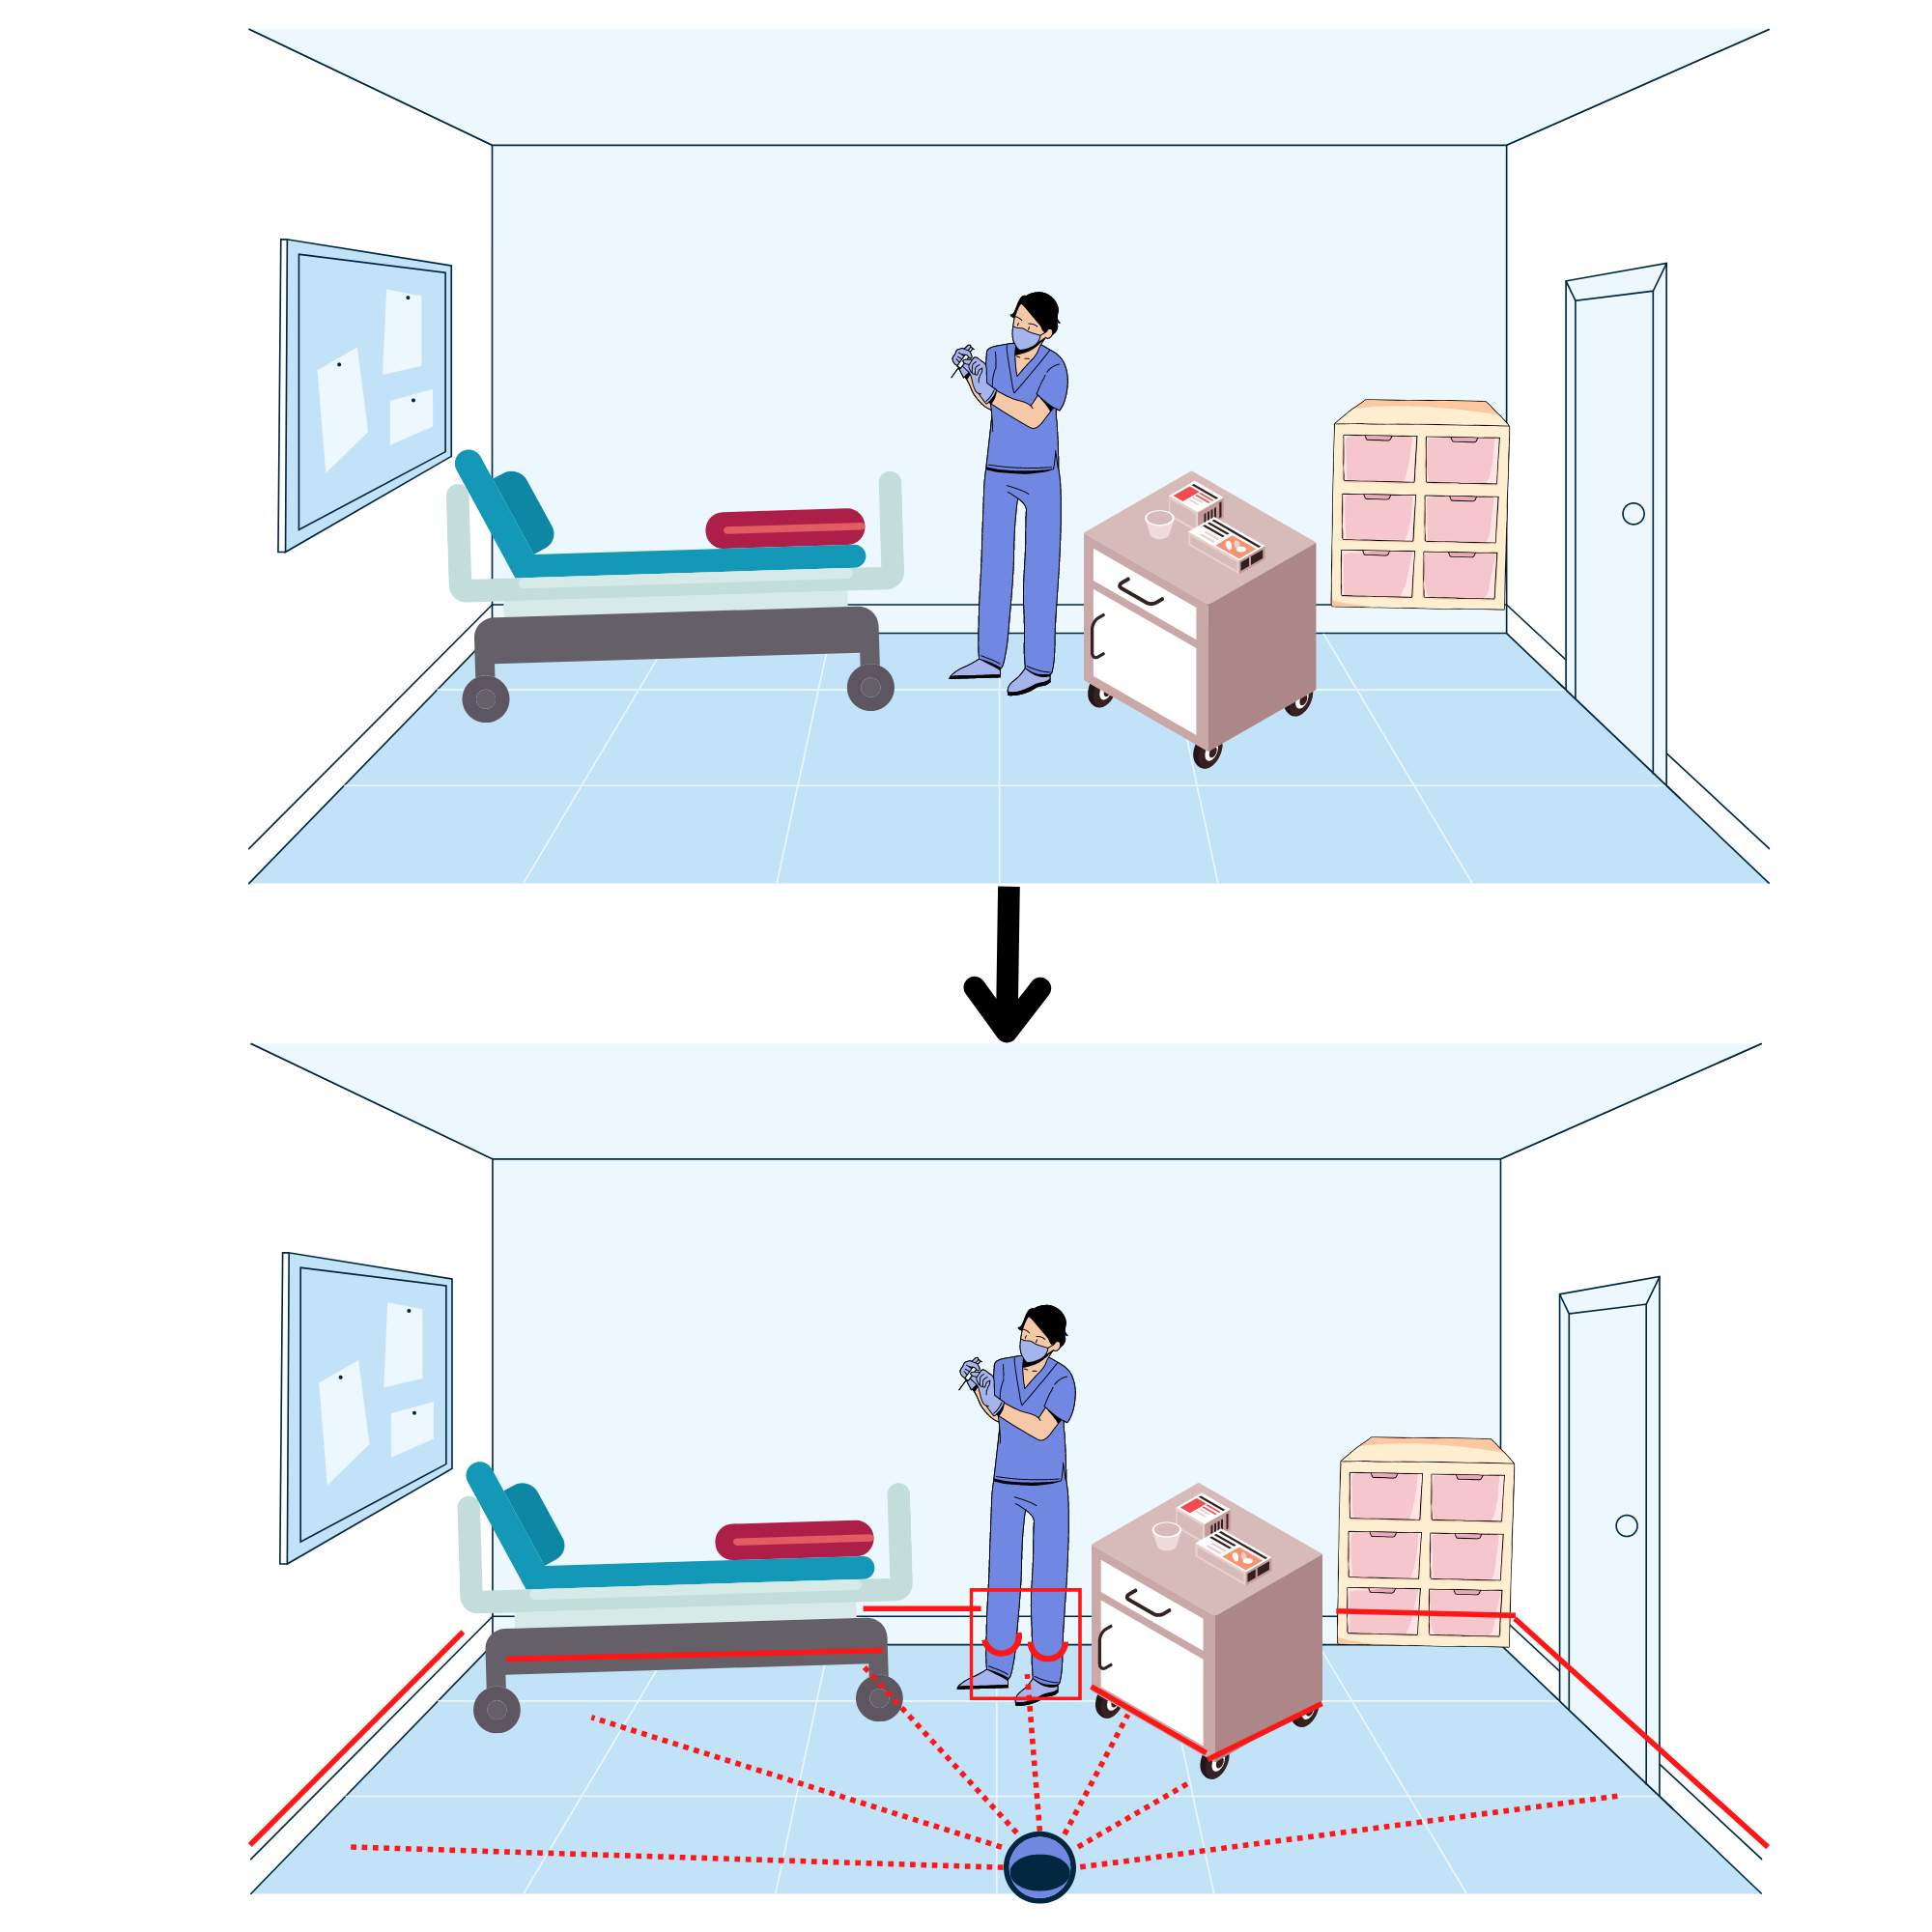
\includegraphics[scale=0.4]{bab4/ilustrasi_L.png}
    \caption{Ilustrasi Kerja Sistem Deteksi.} 
    % source : https://www.canva.com/design/DAFNOD4NtO8/fk5zN3JJ6QSwVgpEgwJ3jg/edit
    \label{fig:Ch04_ilustrasi}
\end{figure}

Pendeteksian dua jenis bentuk yaitu garis dan lingkaran cukup untuk dapat mewakili bentuk-bentuk umum yang biasanya ada di dalam ruangan. Bentuk garis merupakan bentuk umum yang dimiliki berbagai objek di dalam ruangan rumah sakit seperti dinding, meja, tempat tidur, dan sebagainya. Objek-objek dalam ruang yang memiliki bentuk lingkaran cukup terbatas jenisnya. Bentuk lingkaran yang memiliki ukuran seperti manusia juga biasanya jarang ditemukan di lingkungan rumah sakit. Manusia dapat dibedakan dengan objek lingkaran lainnya dengan menambahkan beberapa syarat yang sesuai dengan kriteria kaki manusia.

Sistem deteksi ini secara keseluruhan memiliki empat tahap pembuatan komponen sebelum disimulasikan secara utuh. Tahap-tahap tersebut ditunjukkan pada Gambar \ref{fig:Ch04_sistem_umum}.

    \begin{figure}[H]
        \centering
        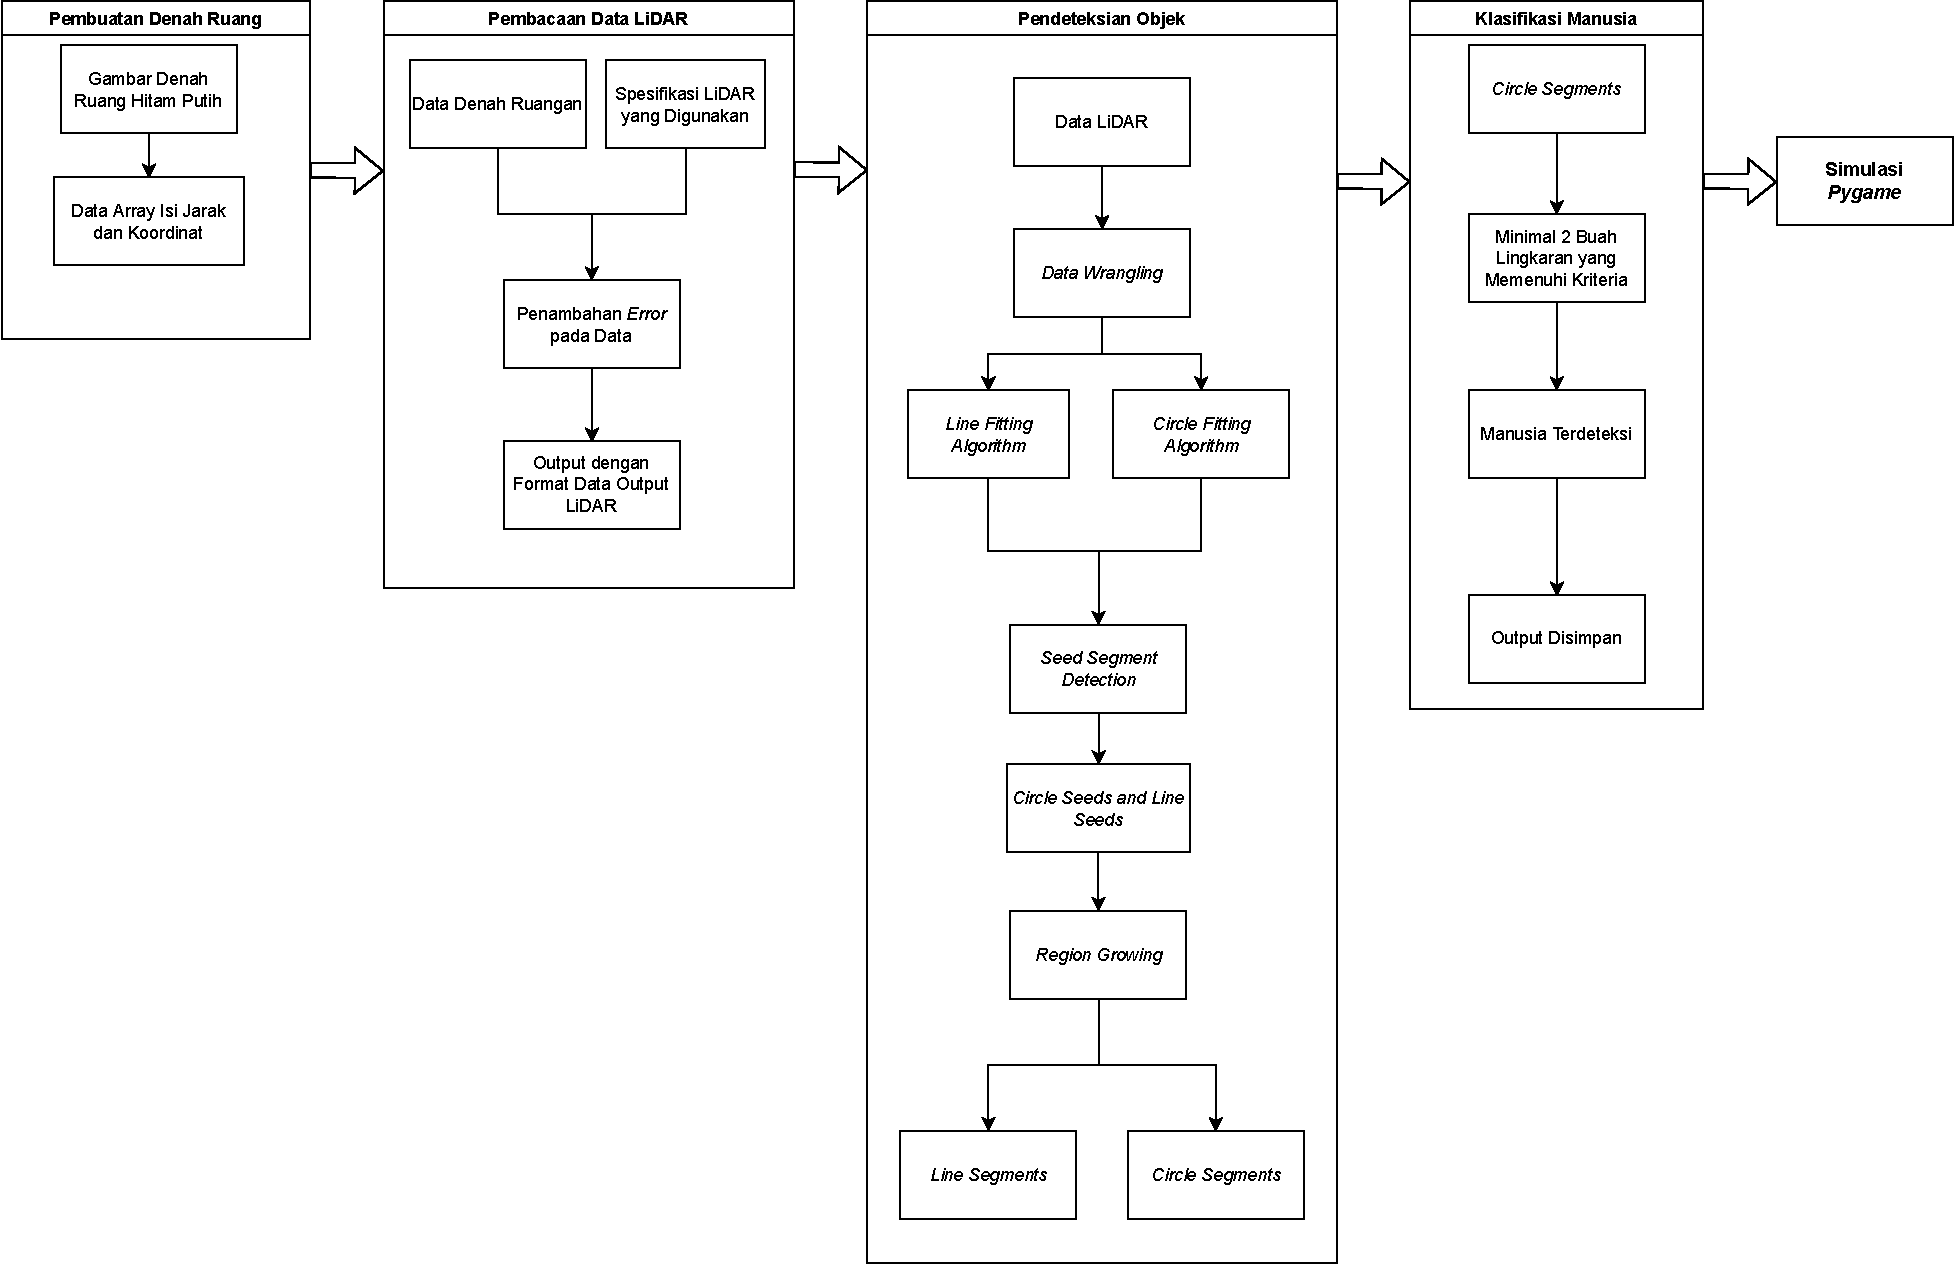
\includegraphics[width=\textwidth]{bab4/workflow_umum.pdf}
        \caption{Diagram Kerja Sistem secara Umum.}
        \label{fig:Ch04_sistem_umum}
    \end{figure}

Tahap pertama adalah pembuatan lingkungan yang akan digunakan. Masukkan data lingkungan untuk simulasi diperoleh dari gambar denah ruangan yang berwarna hitam putih. Gambar kemudian diubah menjadi data \textit{array} agar dapat dengan mudah diproses. Tahap selanjutnya adalah membuat program yang memberi luaran seperti luaran data mentah \lidar. Terdapat dua masukkan yang dibutuhkan untuk membuat program pada tahap ini yaitu data denah ruangan dan spesifikasi \lidar\ yang ingin digunakan. Spesifikasi \lidar\ digunakan sebagai penentu agar data yang dihasilkan dapat memiliki sifat semirip mungkin dengan bacaan \lidar\ asli. Data kemudian ditambah \textit{error} kemudian disusun sesuai format luaran data \lidar. Tahap selanjutnya adalah pendeteksian garis dan lingkaran. Data mentah \lidar\ perlu disusun menjadi format yang mudah diproses. Data-data tersebut akan dimasukkan ke dalam program pendeteksi garis dan lingkaran untuk kemudian dicari apakah ada sekelompok data yang memenuhi kriteria untuk dianggap sebagai \textit{seed}. \textit{Seed} kemudian dikembangkan menjadi garis atau lingkaran, segmen-segmen garis dan lingkaran disimpan untuk diproses pada tahap selanjutnya. Segmen-segmen garis nanti akan ditampilkan pada simulasi sementara segmen-segmen lingkaran akan dikelompokkan terlebih dahulu mana yang memenuhi kriteria untuk dianggap sebagai manusia kemudian ditampilkan pada simulasi. Penjelasan lebih lengkap mengenai diagram kerja dituliskan pada subbab \ref{sec:Persiapan}, subbab \ref{sec:Persiapan2}, subbab \ref{sec:Deteksi}, subbab \ref{sec:Fitting}, dan subbab \ref{sec:Klasifikasi}.

\subsection{Persiapan Denah Ruangan}
\label{sec:Persiapan}

Data proyek \textit{capstone} ini diperoleh tidak menggunakan sensor nyata yang digunakan dalam ruangan, data lingkungan dibuat dari gambar denah ruangan. Denah ruangan dibuat berdasarkan pengamatan dari lorong Gedung DTETI lantai 2. Area yang dijadikan landasan pembuatan denah ditunjukkan area berwarna pada Gambar \ref*{fig:Ch04_lantai_dteti}. 
\begin{figure}[H]
    \centering
    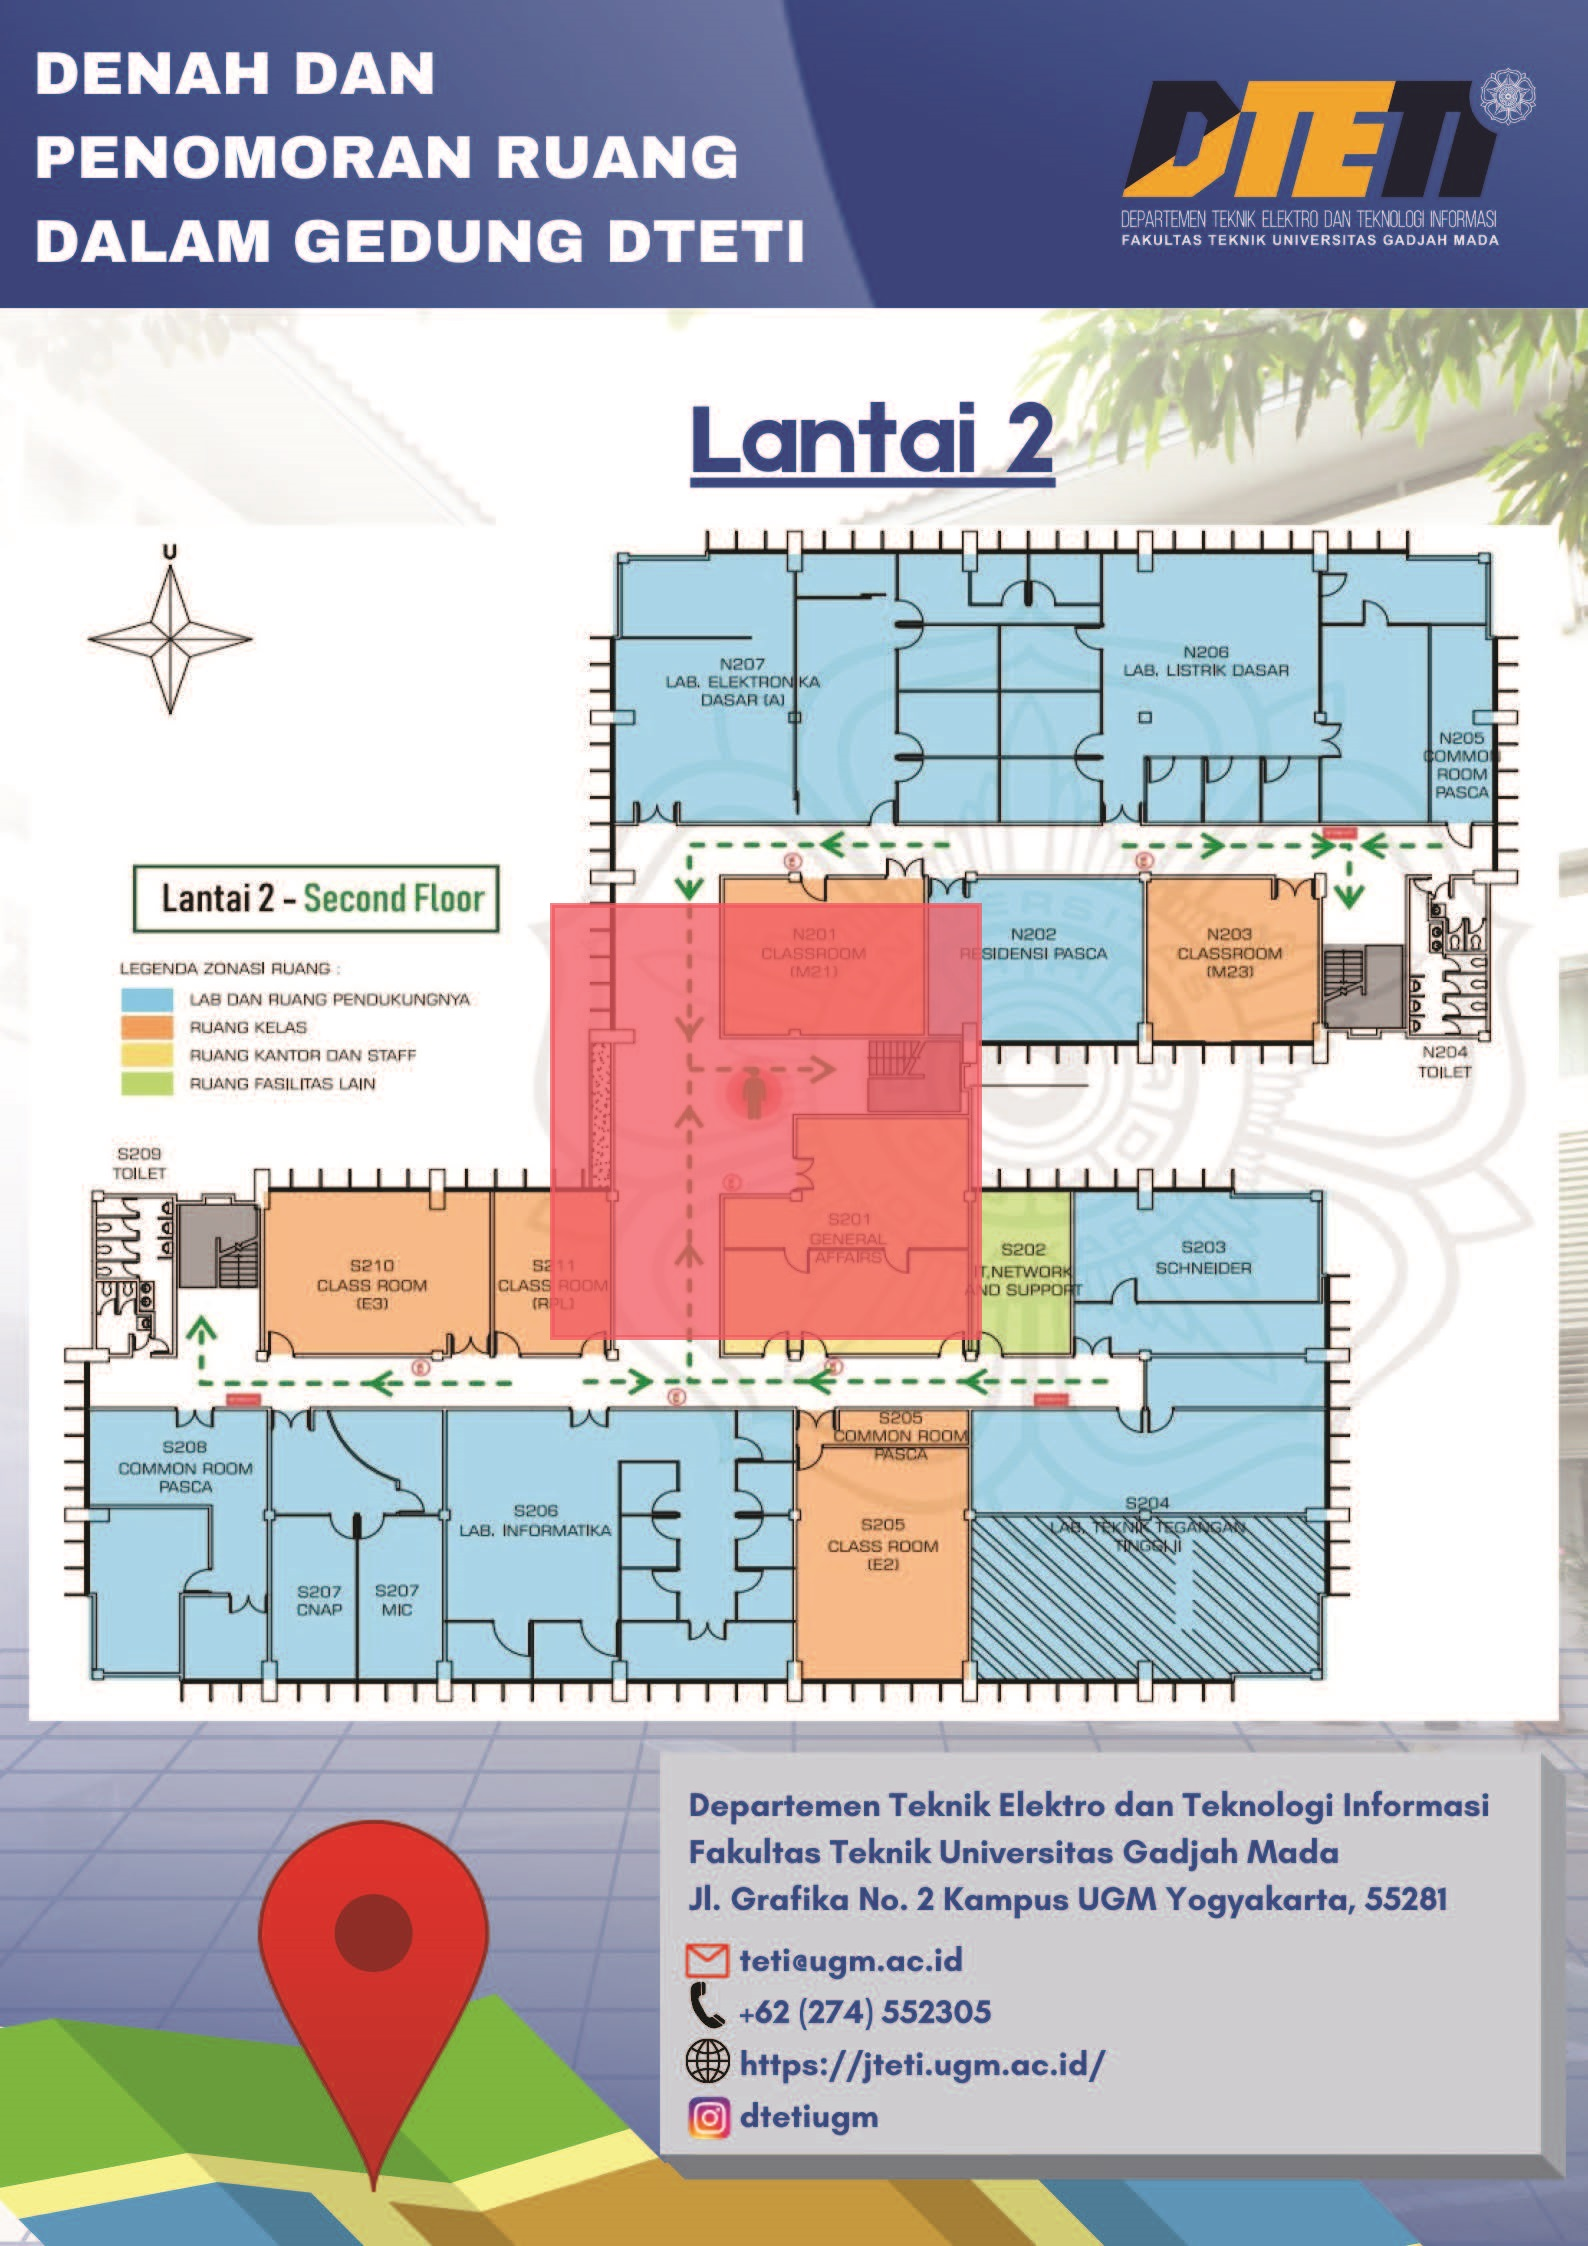
\includegraphics[width=0.7\textwidth]{bab4/denah-lantai-2-rev.jpg}
    \caption{Denah Lantai 2 Gedung DTETI UGM\cite{d00}.}
    \label{fig:Ch04_lantai_dteti}
\end{figure}

Denah ruangan dijadikan landasan ukuran pembuatan lorong yang akan dilalui robot pada simulasi. Denah diubah menjadi berwarna hitam putih dan ditambah beberapa objek berbentuk persegi empat dan lingkaran.
Terlihat pada Gambar \ref{Fig:Ch04_map1}, gambar denah hanya terdiri dari dua warna yaitu hitam dan putih. Warna putih mewakili ruang kosong sementara warna hitam mewakili objek nyata yang menerima pancaran sinar \lidar.

\begin{figure}[H]
    \centering
    \begin{subfigure}[b]{\textwidth}\centering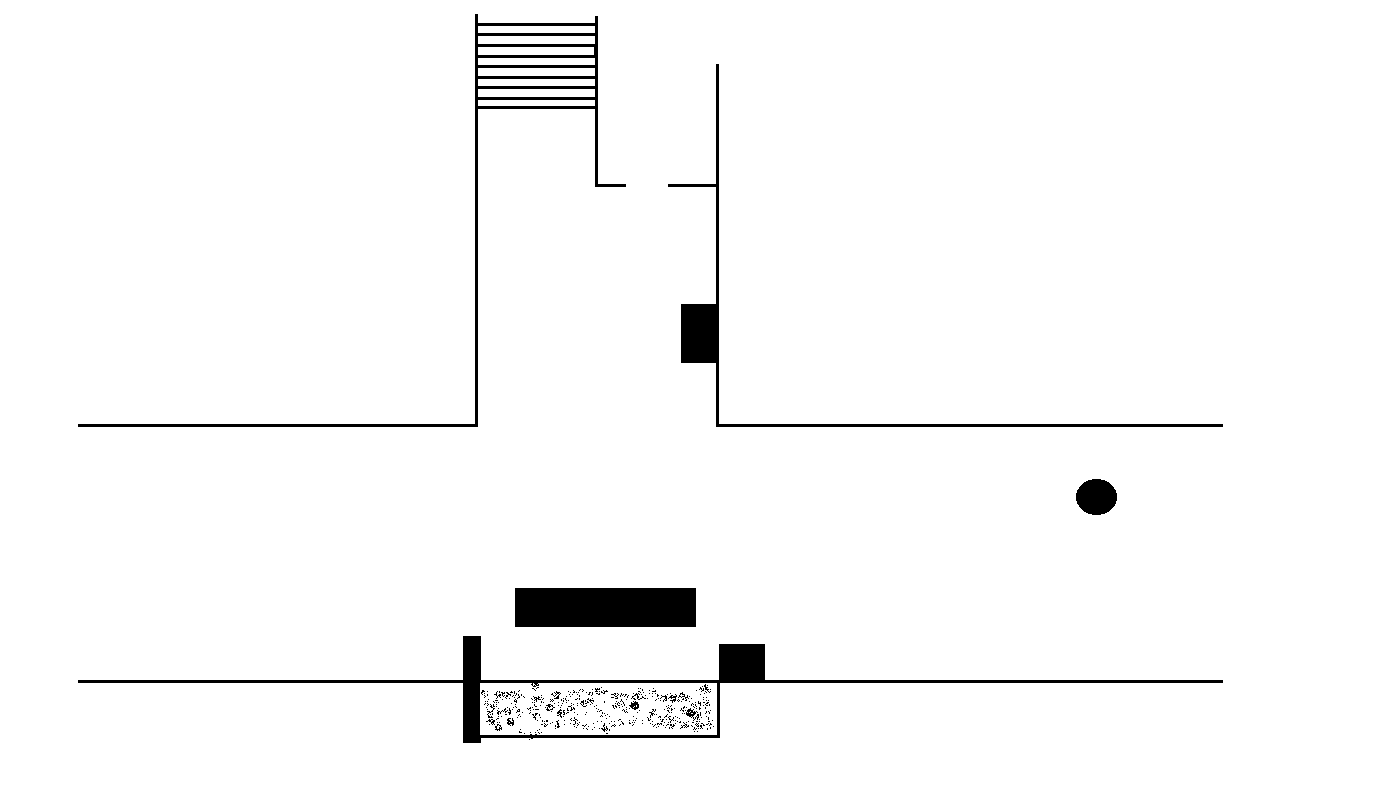
\includegraphics[scale=0.54]{bab4/map_dteti.png}\caption{Denah Ruangan.}\label{Fig:Ch04_map1}\end{subfigure}\\
    \begin{subfigure}[b]{\textwidth}\centering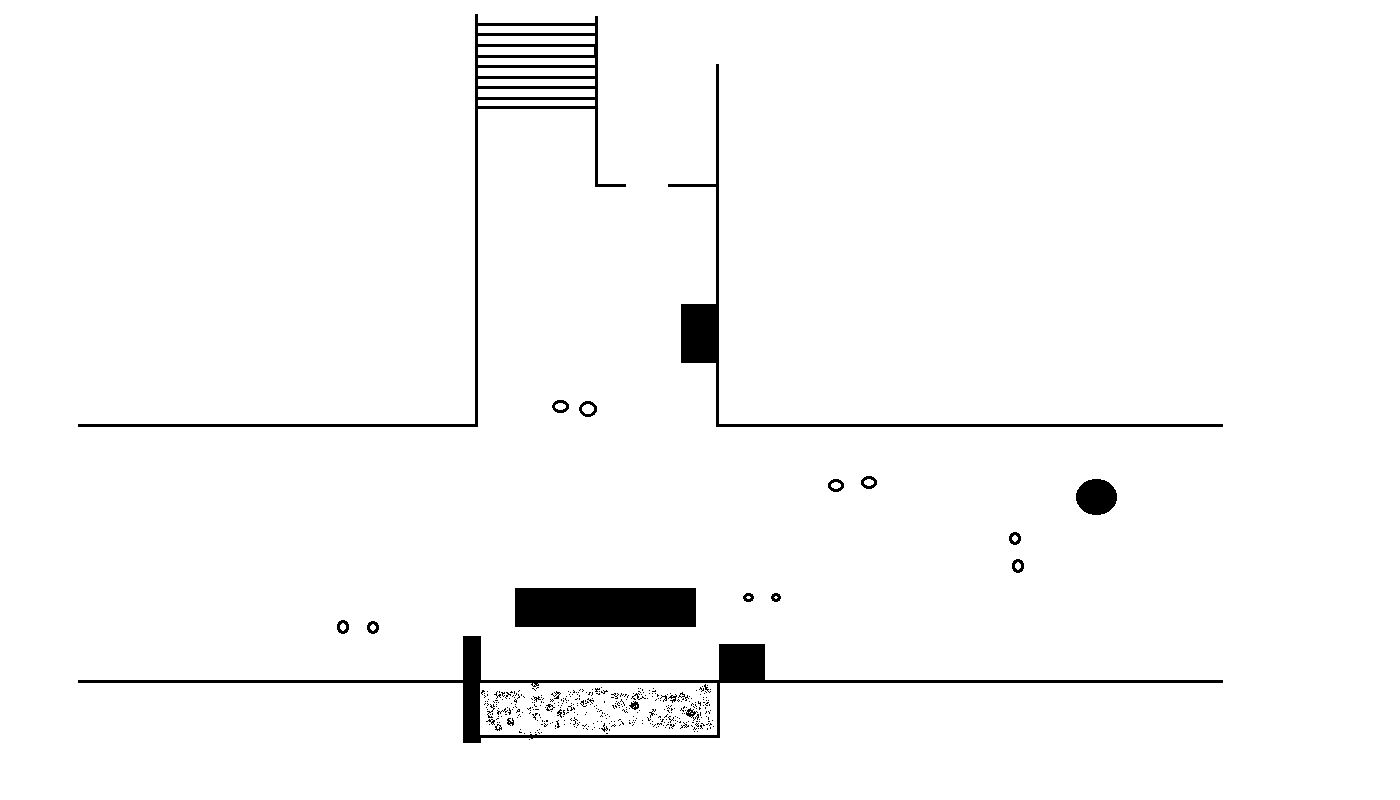
\includegraphics[scale=0.54]{bab4/map_dteti2.png}\caption{Denah Ruangan dengan Manusia.}\label{Fig:Ch04_map2}\end{subfigure}
    \caption{Pembuatan Denah Ruangan}
    \label{fig:Ch04_denahruang}
\end{figure}

Pada Gambar \ref{Fig:Ch04_map2}, manusia ditunjukkan dengan gambar dua buah lingkaran yang berdekatan. Denah awal berisi denah ruangan yang akan dilalui robot, kemudian gambar kedua adalah denah yang sudah ditambahi kaki manusia yang berbentuk sepasang objek lingkaran. Lingkaran-lingkaran ini memiliki jari-jari yang berukuran antara 4,5 cm hingga 8,5 cm. Gambar diproses menjadi data jarak dan posisi objek dengan 1 pixel gambar menggambarkan 1 cm jarak asli.

\begin{figure}[H]
    \centering
    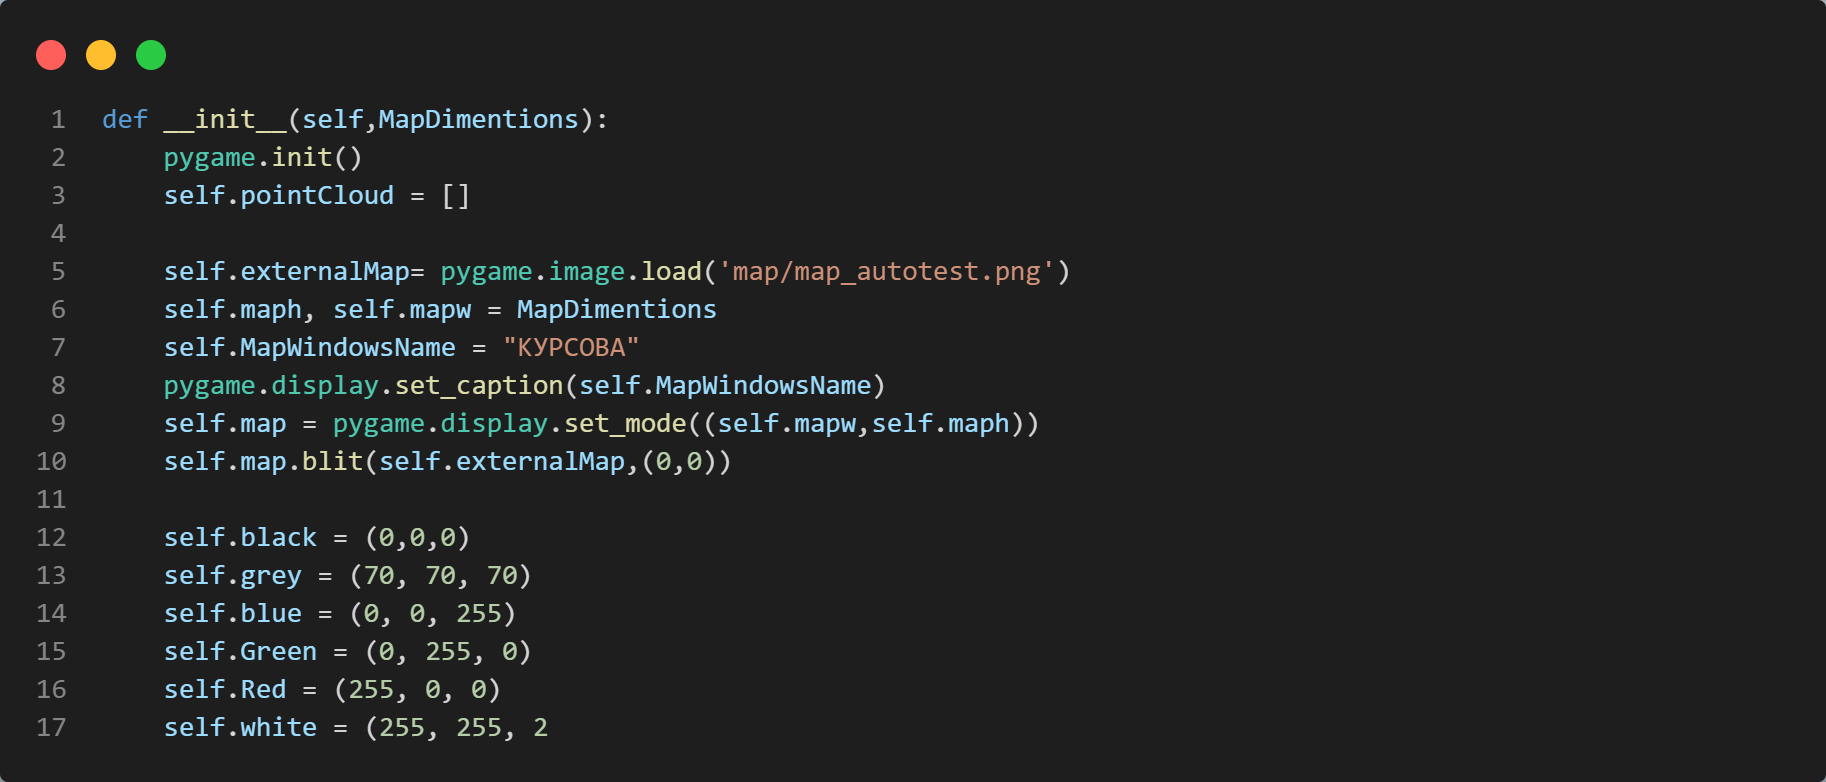
\includegraphics[width=\textwidth]{snippet/build_map.png}
    \caption{Potongan Program Pembacaan Gambar Denah.}
    \label{fig:Ch04_program_denah}
\end{figure}

Potongan program untuk membaca denah yang berupa gambar terlihat pada Gambar \ref{fig:Ch04_program_denah}. Langkah pertama adalah dengan memasukkan gambar png denah ke dalam variabel \textit{self.externalMap} melalui \textit{pygame}. Langkah selanjutnya adalah mengatur ukuran denah dan mengatur nama denah baru yang akan ditampilkan pada layar. Langkah terakhir adalah menggambar data yang diterima dari gambar denah ke tampilan denah yang baru dibuat. Variabel-variabel warna dibuat sebagai persiapan jika nantinya ingin menampilkan warna-warna tersebut dalam denah.
\begin{figure}[H]
    \centering
    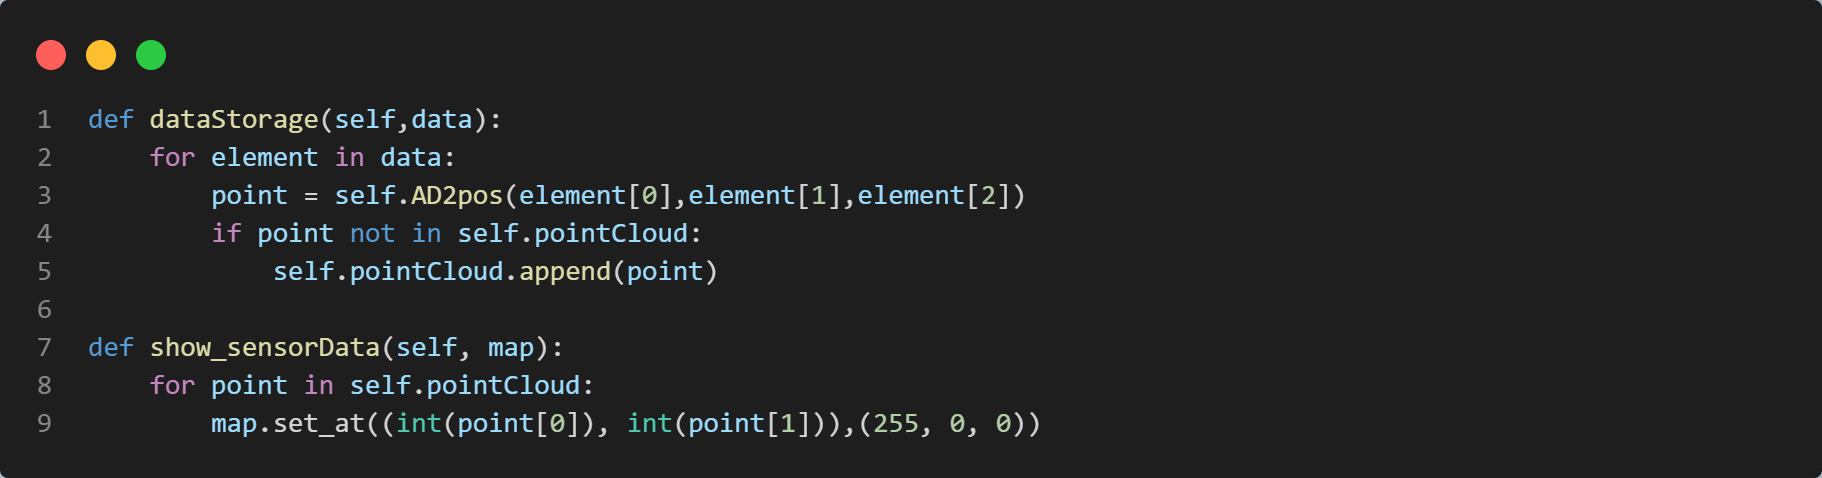
\includegraphics[width=\textwidth]{snippet/build_map2.png}
    \caption{Potongan Program Penyimpanan Data Denah.}
    \label{fig:Ch04_program_denah2}
\end{figure}

Gambar \ref{fig:Ch04_program_denah2} menunjukkan potongan program untuk menyimpan data sebelum ditampilkan pada simulasi. Fungsi \textit{dataStorage} adalah untuk menyimpan hasil bacaan sensor sehingga data pemindaian \lidar\ dari waktu ke waktu tidak akan hilang. Gambar utuh denah ruangan dapat ditampilkan jika fungsi tersebut diaktifkan. Fungsi \textit{show\_sensorData} adalah fungsi yang berguna untuk menampilkan titik-titik yang tersimpan pada fungsi sebelumnya. Titik-titik ini ditampilkan pada simulasi \textit{pygame} dengan warna merah yang diwakilkan pada program dengan kode warna $(255,0,0)$. 


\subsection{Persiapan Data \lidar}
\label{sec:Persiapan2}

Robot akan membaca data lingkungan sesuai spesifikasi \lidar\ yang digunakan. Data objek yang terdeteksi \lidar\ akan dibuat menjadi data yang berisi jarak dan sudut dari objek terdeteksi. Satu putaran \lidar\ memiliki jumlah data yang berbeda-beda sesuai spesifikasi \lidar\ yang digunakan. Jumlah data bacaan \lidar\ yang memiliki jangkauan sudut $360 \degree$ dapat dihitung dengan persamaan \ref*{eqn:SIR1}.
    \begin{align}
        \label{eqn:SIR1}
        Sample\ Rate\ (SR) = \frac{sample\ frequency}{motor\ speed}
    \end{align}
dengan \textit{sample rate} merupakan jumlah data yang diterima dalam satu putaran, \textit{sample frequency} menunjukkan frekuensi kecepatan pembacaan \lidar, dan \textit{motor speed} adalah kecepatan motor dalam \lidar\ untuk memutar laser. 

Nilai jarak dan sudut yang diperoleh \lidar\ akan selalu memiliki nilai ketidakpastian \textit{(uncertainty)}. Nilai ini merupakan perbedaan antara jarak yang diterima \lidar\ dengan jarak asli objek, perbedaan ini dapat diakibatkan oleh berbagai hal seperti kondisi permukaan objek, kualitas manufaktur \lidar, sudut tembakan laser \lidar, dan posisi peletakan \lidar\cite{d0}. Proyek sistem deteksi ini hanya akan memperhitungkan \textit{error} yang dicantumkan pada spesifikasi \lidar. %https://doi.org/10.5194/wes-7-413-2022 
Data yang diperoleh dari objek diam yang dipindai \lidar\ juga dapat memberikan hasil bacaan posisi sudut berbeda dalam setiap pemindaian. Hal ini disebabkan oleh frekuensi penembakkan sinar \lidar\ yang berbeda dengan kecepatan motor yang memutar \lidar\ 2D.

\subsection{Deteksi Segmen Garis dan Lingkaran}
\label{sec:Deteksi}

Ruangan yang telah dibaca oleh \lidar\ hanya akan menghasilkan data mentah yang berisi jarak dan posisi objek yang perlu diproses lebih lanjut agar dapat berguna agar mendukung fungsi-fungsi robot lainnya untuk mengidentifikasi lingkungan. Data yang diperoleh berupa data dua dimensi sehingga objek-objek di sekitar robot hanya dapat dikelompokkan menjadi bentuk-bentuk dua dimensi. 

\begin{figure}[H]
    \centering
    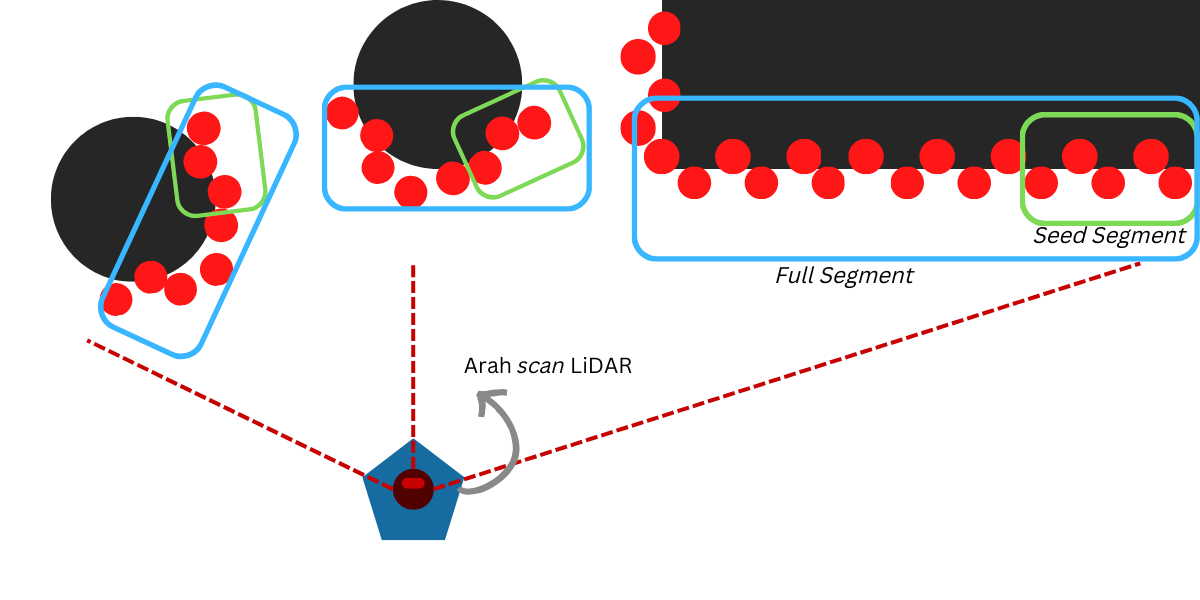
\includegraphics[scale=0.35]{bab4/algoritma.png}
    \caption{Ilustrasi \textit{Seed-growing Algorithm} pada \lidar.}
    \label{fig:Ch04_ilustrasi_algoritma}
\end{figure}

Banyak jenis variasi algoritma yang dapat digunakan untuk mengidentifikasi data 2D \lidar. Proyek \textit{capstone} ini akan menggunakan metode \textit{seed-growing algorithm}\cite{d3}.  
% this paper which uses a variation of the famous split and merge algorithm in order to process 2d lidar data producing a set of line segments that can be used in slam applications this paper claims that this variation can perform better than the original split and merge algorithm in terms of efficiency correctness and precision.\newline 
% BASA BASI:
% Using pure laser scan data to detect human legs can be a 
% complicated problem. Some researchers utilize both vision 
% sensors and laser range scanners [3].
% [3] Kim,  Chung, Detection and tracking of human legs for a mobile service robot[P]. Advanced Intelligent 
% Mechatronics (AIM), 2010 IEEE/ASME International Conference 
% on,2010.
% . Another type of method is to abandon 
% the laser sensor and directly use RGBD-based deep attention 
% models to detect and locate people [4]. This method is more 
% accurate and correspondingly consumes more computing 
% resources than ordinary vision solutions.
% The goal of our work is to build a system that can detect 
% human legs around the robot based on pure laser scan data and 
% minimize false positives. Our leg detection system references 
% the random forest model mentioned above and includes a series 
% of mechanisms like feature filter and map mask to detect human 
% legs without computer vision
% As we can see in Fig 1, our system requires the robot to build
% a two-dimensional map of the surrounding scene using lidar first.
% Then, the robot uses the laser scan data and the already built map 
% to locate itself and update the surrounding environment data in 
% real time.
% The pre-processing process is the process of building a map
% for the environment using the SLAM methods based on the laser 
% scan data.
Algoritma ini secara umum terbagi menjadi dua tahap yaitu \textit{seed-segment detection} dan \textit{region growing} yang dapat dilihat pada Gambar \ref*{fig:Ch04_ilustrasi_algoritma}. \textit{Seed-segment detection} bertujuan untuk mencari kelompok data yang akan digunakan untuk mencari data lain kemudian dimasukkan ke dalam kelompoknya. Setelah kelompok \textit{seed} ditemukan maka selanjutnya dilakukan \textit{region growing}. \textit{Region growing} digunakan untuk mencari titik-titik di sekitar \textit{seed} untuk ditambahkan hingga menjadi segmen garis atau lingkaran yang utuh. Cara kerja kedua tahap tersebut terus diulang-ulang dalam satu kali pembacaan data \lidar\ hingga semua data yang terbaca dapat teridentifikasi. Cara kerja \textit{seed-segment detection} dapat dilihat pada algoritma \ref{algo:algo1} dan cara kerja \textit{region growing} dapat dilihat pada algoritma \ref{algo:algo2}.

\begin{algorithm}[H]
    \caption{Seed-segment Detection} 
    \label{algo:algo1}
    \glsadd{N_p}
    \begin{algorithmic}[1]
        \Require $\textbf{N}_{p}\glsadd{N_p},\epsilon\glsadd{epsilon}, \glsadd{delta}\delta, \glsadd{Snum}S_{num}, \glsadd{Pmin}P_{min}$  
        \State Initialization flag = true
        \For {$i=1 \to (\textbf{N}_{p}\glsadd{N_p}-\textbf{P}_{min})$}
            \State $j \gets i + \textbf{S}_{num}$
            \State fit \glsadd{segmen}\textbf{Seed}$(i,j)$
            \For {$k=i \to j$}
                \State obtain the predicted point or the next point $P'_{k}$
                \State $d_{1} \gets distance\ from\ P_{k}\ to\ P'_{k}$
                \If{$d_{1}>\glsadd{delta}\delta$}
                    \State $flag=false$
                    \State break
                \EndIf
                \State $d_{2}\gets distance\ from\ P_{k}\ to\ \glsadd{segmen}\textbf{Seed} (i,j)$
                \If{$d_{2}>\epsilon\glsadd{epsilon}$}
                    \State $flag = false$
                    \State break
                \EndIf 
            \EndFor
            \If{$flag==true$}
                \State return $\glsadd{segmen}\textbf{Seed} (i,j)$
            \EndIf
        \EndFor
    \end{algorithmic} 
\end{algorithm}

Pada algoritma \ref*{algo:algo1}, $N_p$ merupakan jumlah titik yang terdeteksi. $\glsadd{Snum}S_{num}$ merupakan jumlah titik yang diperlukan untuk \textit{seed-segment} dan $\glsadd{Pmin}P_{min}$ jumlah titik minimal yang dibutuhkan untuk membuat segmen. Segmen garis dari titik $i$ menuju titik $j$ diwakilkan dengan $Seed(i,j)$, sementara nilai $\epsilon\glsadd{epsilon}$ adalah jarak terdekat garis dan $\glsadd{delta}\delta$ adalah jarak antar titik seperti yang dijelaskan pada Gambar \ref{fig:Ch04_epsdelta}.

\begin{figure}[H]
    \centering
    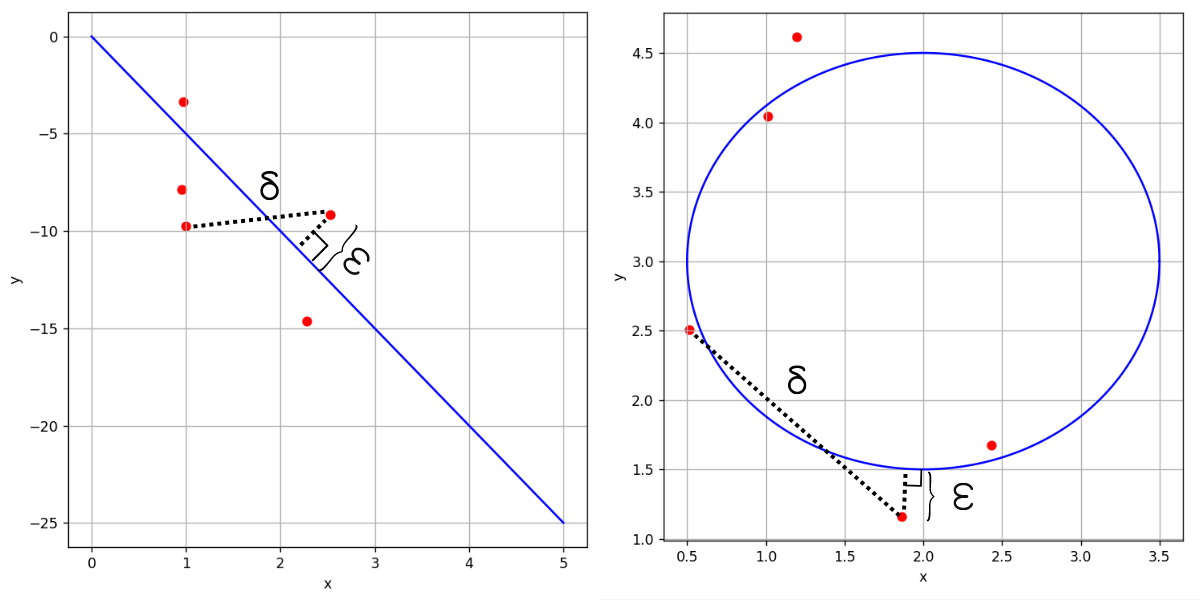
\includegraphics[scale=0.45]{bab4/eps_delta.png}
    \caption{Jarak $\epsilon$ dan $\delta$ pada Garis dan Titik.}
    \label{fig:Ch04_epsdelta}
\end{figure}
Nilai $\epsilon\glsadd{epsilon}_{line}$ dan $\epsilon\glsadd{epsilon}_{circle}$ dapat dihitung menggunakan persamaan jarak titik ke garis dan titik ke lingkaran yang ditampilkan pada Tabel \ref*{tab:Persamaan_Matematis}. Nilai $\glsadd{delta}\delta_{line}$ dan $\glsadd{delta}\delta_{circle}$ dapat juga dilihat pada tabel tersebut yaitu menggunakan rumus jarak titik ke titik. Berbagai persamaan matematika lainnya juga digunakan untuk menyusun sistem deteksi ini. Fungsi dan tujuan persamaan-persamaan tersebut ditampilkan dan dijelaskan pada Tabel \ref*{tab:Persamaan_Matematis}.

\begin{longtable}{|c|L{2cm}|L{4cm}|L{5.5cm}|}
    \caption{Persamaan Matematis dalam \textit{Features Detection}}
    \label{tab:Persamaan_Matematis}
    \vspace{-0.75em}\\
    \hline
   \multicolumn{1}{|c|}{\textbf{No.}} 
   & \multicolumn{1}{|c|}{\textbf{Nama Fungsi}} 
   & \multicolumn{1}{|c|}{\textbf{Fungsi}} 
   & \multicolumn{1}{|c|}{\textbf{Deskripsi}}\\ \hline
    {1.}
      & {Persamaan Garis dengan Gradien} 
      & \multicolumn{1}{|c|}{$y=mx+b$}
      & Persamaan garis lurus dengan $m$ sebagai gradien dan $b$ sebagai titik potong sumbu $y$.
      \\ \hline
    {2.}
    & {Persamaan Garis Umum} 
    & \multicolumn{1}{|c|}{$Ax+By+C=0$}
    & Persamaan garis dalam bentuk umum di bidang sumbu $x$ dan $y$.
    \\ \hline
    {3.}
    & {Persamaan Garis dari Dua Titik} 
    & \multicolumn{1}{|c|}{\large$\frac{y-y_1}{y_2-y_1}=\frac{x-x_1}{x_2-x_1}$}
    & Persamaan garis yang dapat diperoleh jika diketahui dua titik $(x_1,y_1)$ dan $(x_2,y_2)$. 
    \\ \hline
    {4.}
    & {Jarak Titik ke Titik} 
    & \multicolumn{1}{|c|}{$\sqrt{(x_2-x_1)^2+(y_2-y_1)^2}$}
    & Persamaan untuk menghitung jarak antar dua titik yaitu titik $(x_1,y_1)$ dan $(x_2,y_2)$.
    \\ \hline
    {5.}
    & {Jarak Titik ke Garis}
    & \multicolumn{1}{|c|}{\large$\frac{|Ax_i+By_i+C|}{\sqrt{A^2+B^2}}$}
    & Persamaan untuk menghitung jarak dari sebuah titik $(x_i,y_i)$ menuju sebuah garis dengan persamaan $Ax+By+C=0$.
    \\ \hline
    {6.}
    & {Jarak Titik ke Lingkaran}
    & \multicolumn{1}{|c|}{$\sqrt{|(x_i-x_c\glsadd{x_c})^2+(y_i-y_c\glsadd{y_c})^2|}-r_c\glsadd{r_c}$}
    & Persamaan untuk menghitung jarak dari sebuah titik $(x_i,y_i)$ menuju sebuah lingkaran dengan persamaan $(x-x_c)^2+(y-y_c)^2+R^2=0$.
    \\ \hline
    {7.}
    & {Jarak Titik ke Titik dalam Busur Lingkaran}
    & \multicolumn{1}{|c|}{
        \begin{tabular}{c}
            \small $\theta\glsadd{theta}=\arctan \left(\frac{\mfrac{y_c\glsadd{y_c}-y_2}{x_c\glsadd{x_c}-x_2} - \mfrac{y_c\glsadd{y_c}-y_1}{x_c\glsadd{x_c}-x_1}}{1+\left(\mfrac{y_c\glsadd{y_c}-y_2}{x_c\glsadd{x_c}-x_2}\right) \left(\mfrac{y_c\glsadd{y_c}-y_1}{x_c\glsadd{x_c}-x_1}\right)}\right)$\\ \\
            $jarak = \left(\frac{\theta\glsadd{theta}}{360\degree}\right)\times 2\pi r_c\glsadd{r_c}$
        \end{tabular}}
    & Persamaan untuk menghitung jarak busur lingkaran dengan pusat $(x_c\glsadd{x_c},y_c\glsadd{y_c})$ dan jari-jari $r_c\glsadd{r_c}$. Sebuah busur tersebut memiliki dua titik di ujung yaitu titik $(x_1,y_1)$ dan titik lain $(x_2,y_2)$.
    \\ \hline

    {8.}
    & {Titik Potong Dua Garis}
    & \multicolumn{1}{|c|}{$
        \begin{pmatrix}
          -m_1 & 1\\
          -m_2 & 1
        \end{pmatrix}
        \begin{pmatrix}
            x_k\\
            y_k
          \end{pmatrix} =
        \begin{pmatrix}
            b_1\\
            b_2
          \end{pmatrix}
      $}
    & Titik perpotongan antara dua persamaan garis $y=m_1x+b_1$ dan $y=m_2x+b_2$ dapat digambarkan dengan persamaan matriks tersebut yang nantinya dapat menghasilkan titik perpotongan $(x_k,y_k)$.
    \\ \hline
    {9.}
    & {Proyeksi Titik ke Garis}
    & \multicolumn{1}{|c|}{
        \begin{tabular}{c}
        $m_2=-\frac{1}{m}$\\ \\
        $y = m_2x+c_2$\\ \\
        $x_{k} = -\frac{(b-c_2)}{(m-m2)}$\\ \\
        $y_{k} = m_2x_{k}+c_2$
        \end{tabular} }
    & Fungsi untuk menghitung titik proyeksi $(x_k,y_k)$ dari sebuah titik $(x,y)$ di luar sebuah garis $y=mx+b$ sehingga apabila ditarik garis dari titik $(x,y)$ menuju $(x_k,y_k)$ maka garis tersebut akan tegak lurus dengan garis $y=mx+b$.
    \\ \hline

    {10.}
    & {Proyeksi Titik ke Lingkaran}
    & \multicolumn{1}{|c|}{
        \begin{tabular}{c}
        $\theta\glsadd{theta} = arctan \left( \frac{y_i-y_c\glsadd{y_c}}{x_i-x_c\glsadd{x_c}}\right)$\\ \\
        $x_{k} = x_c\glsadd{x_c} + r_c\glsadd{r_c} \cos \theta\glsadd{theta}$\\ \\
        $y_{k} = y_c\glsadd{y_c} + r_c\glsadd{r_c} \sin \theta\glsadd{theta}$
        \end{tabular} }
    & Fungsi untuk menghitung titik proyeksi $(x_k,y_k)$ dari sebuah titik $(x_i,y_i)$ di luar sebuah lingkaran $(x-x_c)^2+(y-y_c)^2+R^2=0$ sehingga apabila ditarik garis dari titik $(x,y)$ menuju $(x_k,y_k)$ maka jarak garis tersebut adalah jarak terdekat titik $(x_i,y_i)$ dengan lingkaran.
    \\ \hline

    {11.}
    & {Koordinat Polar dan Kartesius}
    & \multicolumn{1}{|c|}{
        \begin{tabular}{c}
            $x = r\ cos \theta\glsadd{theta}$\\ \\ 
            $y = r\ sin \theta\glsadd{theta}$
        \end{tabular}}
    & Fungsi untuk mengubah hasil bacaan \lidar\ yang berupa koordinat polar menjadi koordinat kartesius sehingga lebih mudah untuk diproses.
    \\ \hline
   \end{longtable}
Tabel \ref*{tab:Persamaan_Matematis} menjelaskan jenis-jenis persamaan yang digunakan dalam program. Persamaan-persamaan ini digunakan untuk membantu perhitungan dan memperoleh data dari kumpulan titik-titik yang dibaca \lidar. Persamaan-persamaan tersebut berfungsi dari proses pembacaan data \lidar\ hingga proses klasifikasi manusia.

\begin{algorithm}[H]
    \caption{Region Growing} 
    \label{algo:algo2}
    \begin{algorithmic}[1]
        \Require $\glsadd{segmen}\textbf{Seed} (i,j),\textbf{N}_{p}\glsadd{N_p}, \textbf{P}_{min}, \textbf{L}_{min}, \epsilon\glsadd{epsilon}$ 
        \State Initialization: $\textbf{Line}(P_{b},P_{f})\gets \glsadd{segmen}\textbf{Seed} (i,j),\textbf{L}_{l}=0, \textbf{P}_{l}=0 $
        \State $\textbf{P}_{f}=j+1, \textbf{P}_{b}=i-1$
        \While{$distance(\textbf{P}_{f}, \textbf{Line}<\epsilon\glsadd{epsilon})$}
            \If{$\textbf{P}_{f}>\textbf{N}_{p}\glsadd{N_p}$}
                \State break
            \Else
                \State refit $\textbf{Line}(\textbf{P}_{b}, \textbf{P}_{f})$
            \EndIf
            \State $P_{f} \gets P_{f}+1$
        \EndWhile
        \State $P_{f} \gets P_{f} -1 $
        \While{$distance(\textbf{P}_{b}, \textbf{Line}<\epsilon\glsadd{epsilon})$}
            \If{$\textbf{P}_{b}<1$}
                \State break
            \Else
                \State refit $\textbf{Line}(\textbf{P}_{b}, \textbf{P}_{f})$
            \EndIf
            \State $P_{f} \gets P_{f}-1$
        \EndWhile
        \State $P_{b} \gets P_{b}+1$
        \State obtain $\textbf{L}_{l}, \textbf{P}_{l}$ from $\textbf{Line}(\textbf{P}_{b}, \textbf{P}_{f})$
        \If{$(\textbf{L}_{l} \geq \textbf{L}_{min}) \& (\textbf{P}_{l} \geq \textbf{P}_{min})$}
            \State \Return $\textbf{Line}(\textbf{P}_{b}, \textbf{P}_{f})$ with $\textbf{Parameters}(a,b,c)$
        \EndIf

    \end{algorithmic}
\end{algorithm}

Setelah \textit{seed-segment} diperoleh, maka langkah selanjutnya adalah melanjutkan pengumpulan titik-titik di sekitarnya dan menggabungkannya dengan segmen apabila memenuhi syarat. Terlihat pada algoritma \ref*{algo:algo2} bahwa syarat yang diperlukan yaitu jarak titik dengan garis kurang dari $\epsilon\glsadd{epsilon}$. Segmen dikembangkan dari dua sisi yaitu titik awal $P_b$ dan titik akhir $P_f$. $L_{min}$ dan $L_l$ merepresentasikan panjang minimal gari dan panjang asli garis yang dibentuk segmen. $P_l$ adalah jumlah titik yang dimiliki segmen yang sedang dikembangkan. 


% algoritma overlap region growing:

% \begin{algorithm}
%     \caption{Overlap Region Growing} 
%     \label{algo:algo2}
%     \begin{algorithmic}[1]
%         \Require $\textbf{N}$ (the number of line segments) 
%         \For{$i=1 \to \textbf{N}_l - 1$}
%             \State $j \gets i-1$
%             \State Endpoint index of $\textbf{Line}_i : (m_1,n_1)$
%             \State Endpoint index of $\textbf{Line}_j : (m_2,n_2)$
%         \If{$m_2 \leq n_1$}
%             \For{$k=m_2 \to n_1$}
%                 \State $d^i_k=$distance$(\textbf{P}_k,\textbf{Line}_i)$ 
%                 \State $d^j_k=$distance$(\textbf{P}_k,\textbf{Line}_j)$ 
%                 \If{$^i_k<d^j_k$}
%                     \State continue
%                 \Else
%                     \State break
%                 \EndIf
%             \EndFor
%             \State $n_1 \gets k-1$
%             \State $m_2 \gets k$
%         \Else
%             \State break
%         \EndIf
%         \State refit $\textbf{Line}(m_1,n_1)$
%         \State refit $\textbf{Line}(m_2,n_2)$
%     \EndFor
%     \State \Return line segments without overlap region
%     \end{algorithmic}
% \end{algorithm}
\subsection{\textit{Orthogonal Distance Regression} dan \textit{Least-square Circle Fitting}}
\label{sec:Fitting}
Agar sistem dapat memperoleh bentuk garis dan lingkaran diperlukan juga algoritma \textit{fitting}. \textit{Orthogonal Distance Regression (ODR)} digunakan untuk memperoleh persamaan garis dalam sebuah kelompok titik dengan meminimalkan \textit{error} garis tersebut terhadap titik sekitarnya. Terlihat pada Gambar \ref*{fig:Ch04_odr}, \textit{error} dihitung dari jarak terdekat titik dengan garis\cite{d1}.%https://www.wavemetrics.com/products/igorpro/dataanalysis/curvefitting/errorsinvariables

\begin{figure}[H]
    \centering
    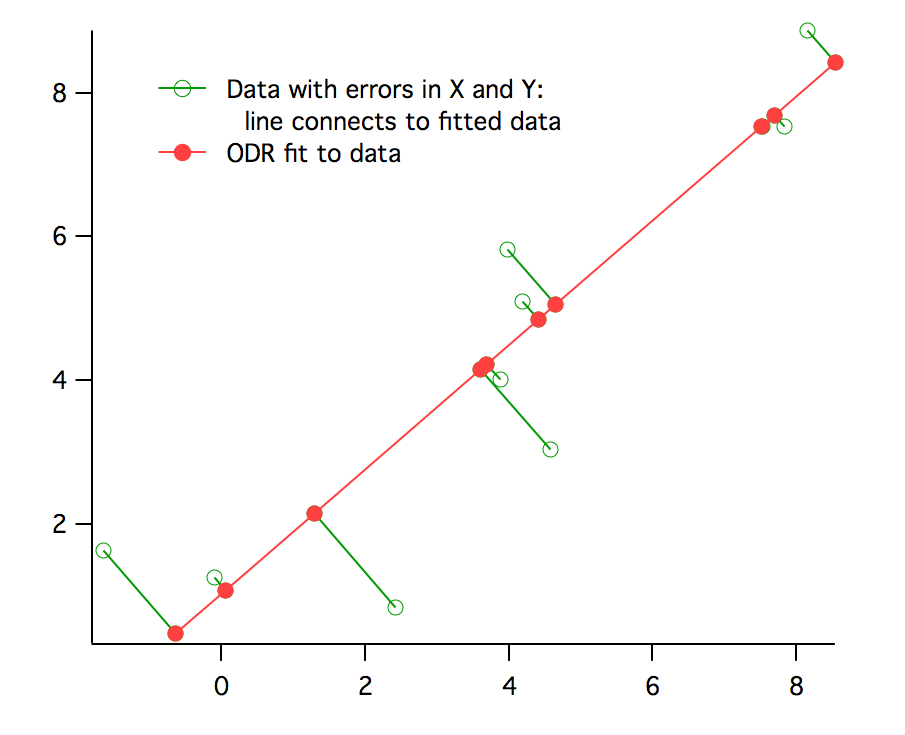
\includegraphics[scale=0.6]{bab4/odr_fit.png}
    \caption{ODR \textit{Fitting}.}
    \label{fig:Ch04_odr}
\end{figure}
ODR menentukan persamaan garis dengan meminimalkan jarak titik ke persamaan garis. Persamaan garis yang diregresi pada \capstone\ ini merupakan persamaan garis lurus yang ditampilkan pada persamaan \ref{eq:garis_lurus}.
\begin{equation}
    \label{eq:garis_lurus}
    y=mx+b
\end{equation}
kemudian garis tegak lurus dicari dengan memberi nilai gradien baru $-\frac{1}{m}$ kemudian dicari titik pada data $(x_0,y_0)$ data dan dibuat persamaan garis yang melalui data dengan gradien tegak lurus seperti yang terlihat pada persamaan \ref{eq:garis_tegak_lurus}.
\begin{equation}
    \label{eq:garis_tegak_lurus}
    y=-\frac{x}{m}+(\frac{x_0}{m}+y_0)
\end{equation}
Koordinat perpotongan garis regresi dengan persamaan garis tegak lurus dapat dicari dengan persamaan \ref*{eqn:ODR}.
\begin{equation}
    \label{eqn:ODR}
    \begin{gathered}
        x_i = \frac{(x_0 + my_0 - m*b)}{(m^2 + 1)}\\
        y_i = m*y_i + b       
    \end{gathered}
\end{equation}
Langkah selanjutnya setelah menemukan titik potong $(x_i,y_i)$ adalah mencari jarak dengan titik $(x_0,y_0)$ pada data hasil bacaan. Persamaan garis diregresi hingga menghasilkan nilai jarak paling minimum dari total titik-titik yang termasuk area garis tersebut.

% https://www.geeksforgeeks.org/orthogonal-distance-regression-using-scipy/

Identifikasi bentuk lingkaran pada data dilakukan dengan metode \textit{Least-square}\cite{d2}. %https://scipy-cookbook.readthedocs.io/items/Least_Squares_Circle.html
Sekelompok titik yang terletak pada $\glsadd{lokasi_r2}\mathbb{R}^2$ dapat dikatakan sebagai  $ \{(x_i,y_i)|0 \leq i \leq N\}$ dengan
$0\leq i \leq N$ menunjukkan data dari 0 hingga $N$. Titik-titik ini digunakan untuk mencari bentuk lingkaran yang paling sesuai untuk mewakilinya yang dituliskan sebagai persamaan \ref*{eqn:Circle} dengan $(x_c\glsadd{x_c},y_c\glsadd{y_c})$ sebagai koordinat pusat lingkaran dan $R$ sebagai jari-jari lingkaran. 
\begin{equation}
    \label{eqn:Circle}
    (x-x_c)^2+(y-y_c)^2+R^2=0
\end{equation}
Langkah pertama \textit{circle fitting} adalah dengan mengasumsikan nilai baru $u$ dan $v$ menjadi:
\begin{equation}
    \begin{gathered}
        u_i=x_i-\bar{x}, \\ 
        v_i=y_i-\bar{y}
        \label{eqn:asumsi_uv}
    \end{gathered} 
\end{equation}

 \begin{tabbing}
dengan: \=\\
    \>$i$ \qquad \qquad \qquad \=: menunjukkan titik ke-$i$,\\ 
    \>$\bar{x}=\frac{1}{N}\sum_{i=1}^n x_i$      \>: nilai rata-rata titik $x$ dari titik pertama hingga titik terakhir $n$,\\
    \>$\bar{y}=\frac{1}{N}\sum_{i=1}^n y_i$      \>: nilai rata-rata titik $y$ dari titik pertama hingga titik terakhir $n$.
 \end{tabbing}
%  $\bar{x}=\frac{1}{N}\sum_i x_i$ dan $\bar{y}=\frac{1}{N}\sum_i y_i$ merupakan rata-rata nilai $x$ dan $y$.
% rumus circle fitting AllahuAkbar:
% Given a finite set of points in $\glsadd{lokasi_r2}\mathbb{R}^2$ ,say $ \{(x_i,y_i)|0 \leq i \leq N\}$\\
% we estimate the best circle : $(x-x_c\glsadd{x_c})^2+(y-y_c\glsadd{y_c})^2+R^2=0$ define: $\bar{x}=\frac{1}{N}\sum_i x_i$ and $\bar{y}=\frac{1}{N}\sum_i y_i$
% dengan $u_i=x_i-\bar{x}, v_i=y_i-\bar{y}\ for\ 0\leq i \leq N$ 
% We solve the problem first in (u, v) coordinates, and then transform back to (x, y)\\
Persamaan diselesaikan dalam koordinat $(u,v)$ dan kemudian dikembalikan ke koordinat $(x,y)$. Lingkaran baru memiliki koordinat titik tengah $(u_c, v_c)$ dan jari-jari $R$, maka nilai yang ingin diminimalkan adalah:
\begin{equation}
    \begin{gathered}
        S=\sum_{i=1}^n ((u_i-u_c)^2+(v_i-v_c)^2+\alpha)^2\\
        \alpha=R^2
        \label{eqn:yang_diminimalkan}
    \end{gathered} 
\end{equation}
dengan nilai $S$ merupakan jarak titik $(u_i, v_i)$ dengan lingkaran. Hal tersebut dapat dicapai dengan melakukan diferensial pada $S(\alpha, u_c, v_c)$. Permasalahan kemudian diselesaikan dengan memberi nilai diferensial setiap parameter menjadi:
\begin{equation}
    \begin{gathered}
        \frac{\partial S}{\partial \alpha} =0,\\ 
        \frac{\partial S}{\partial u_c} =0,\\
        \frac{\partial S}{\partial v_c} =0
        \label{eqn:yang_diferensial}
    \end{gathered} 
\end{equation}
sehingga menghasilkan persamaan yang tertulis pada persamaan \ref*{eqn:turunan1}, \ref*{eqn:turunan2}, dan \ref*{eqn:turunan3}.

\begin{align}
    \label{eqn:turunan1}
    \sum_{i=1}^n ((u_i-u_c)^2+(v_i-v_c)^2-\alpha)=0, \\
    \label{eqn:turunan2}
    \sum_{i=1}^n u_i((u_i-u_c)^2+(v_i-v_c)^2-\alpha)=0, \\
    \label{eqn:turunan3}
    \sum_{i=1}^n v_i((u_i-u_c)^2+(v_i-v_c)^2-\alpha)=0.
\end{align}

% Let the circle have center  and radius R. We want to minimize $S=\sum_i (g(u_i,v_i))^2$  $g(u,v)=(u-u_c)^2+(v-v_c)^2+\alpha$  $\alpha=R^2$\\. 
% To do that, we differentiate $S(\alpha, u_c, v_c).$\\
% this problem is solved by setting the derivation of each parameter to zero: $\frac{\partial S}{\partial \alpha} =0, \frac{\partial S}{\partial u_c} =0, and \frac{\partial S}{\partial v_c} =0 $ sehingga:\\
% $
% \sum_i=1^n ((u_i-u_c)^2+(v_i-v_c)^2-\alpha)=0, \newline
% \sum_i=1^n u_i((u_i-u_c)^2+(v_i-v_c)^2-\alpha)=0, \newline
% \sum_i=1^n v_i((u_i-u_c)^2+(v_i-v_c)^2-\alpha)=0,
% $
Pusat lingkaran dapat diperoleh dengan menyelesaikan persamaan \ref*{eqn:turunan2} dan \ref*{eqn:turunan3} yang menghasilkan persamaan \ref*{eqn:pusat_uv} dan \ref*{eqn:pusat_uv2}.
\begin{align}
    \label{eqn:pusat_uv}
    u_c=\frac{S_{uuv}S_{uv}-S_{uuu}S_{vv}-S_{uvv}S_{vv}+S_{uv}S_{vvv}}{2(S^2_{uv}-S_{uu}S_{vv})}\\
    \label{eqn:pusat_uv2}
    v_c=\frac{-S_{uu}S_{uuv}-S_{uuu}S_{uv}-S_{uv}S_{uvv}+S_{uu}S_{vvv}}{2(S^2_{uv}-S_{uu}S_{vv})}.
\end{align}
\begin{tabbing}
    dengan \=variabel-variabel baru yang didefinisikan sebagai berikut:\\
    
    \>$S_u = \sum_{i=1}^n u_i$,\\
    \>$Sv = \sum_{i=1}^n v_i$,\\
    \>$S_{uu} = \sum_{i=1}^n u_i^2$,\\
    \>$S_{vv} = \sum_{i=1}^n v_i^2$,\\
    \>$S_{uv} = \sum_{i=1}^n u_i v_i$,\\
    \>$S_{uuu} = \sum_{i=1}^n u_i^3$,\\
    \>$S_{vvv} = \sum_{i=1}^n v_i^3$,\\
    \>$S_{uvv} = \sum_{i=1}^n u_i v_i^2$,\\
    \>$S_{vuu} = \sum_{i=1}^n v_i u_i^2$.
\end{tabbing}
% can be rewritten like:
% $S_{uuu} - 2u_c S_{uu}+u_c^2S_u+S_{uvv}-2v_cS_{uv}+v_c^2S_u-\alpha S_u=0$\\
% $S_u=0,$ maka simplify:
% $\\ u_cS_{uu}+v_c S_{uv}=\frac{1}{2}(S_{uuu}+S_{uvv})$\\
%
% $S_v=0,$ maka simplify:
% $\\ u_cS_{uv}+v_c S_{uv}=\frac{1}{2}(S_{vvv}+S_{vuu})$\\
% jadi 
% $
% u_c=\frac{S_{uuv}S_{uv}-S_{uuu}S_{vv}-S_{uvv}S_{vv}+S_{uv}S_{vvv}}{2(S^2_{uv}-S_{uu}S_{vv})}\\
% v_c=\frac{-S_{uu}S_{uuv}-S_{uuu}S_{uv}-S_{uv}S_{uvv}+S_{uu}S_{vvv}}{2(S^2_{uv}-S_{uu}S_{vv})}\\
% $
Radius lingkaran $(u_c, v_c)^T$ akhirnya dapat diperoleh ketika $S_{uuu}S_{vu}-S^2_{uv} \neq 0,$ persamaan dibawa kembali ke koordinat $(x,y)$ sehingga nilai titik pusat $(x_c\glsadd{x_c},y_c\glsadd{y_c})$ dan radius lingkaran ($R$) dituliskan sebagai berikut:
\begin{align}
    \label{eqn:final_circle_equation}
    (x_c\glsadd{x_c},y_c\glsadd{y_c})^T=(u_c,v_c)^T+(\bar{x},\bar{y})^T\\
    R=\sqrt{\alpha}=\sqrt{u_c^2+v_c^2+\frac{S_{uu}+S_{vv}}{n}}.
\end{align}

\subsection{Klasifikasi Manusia}
\label{sec:Klasifikasi}

Langkah terakhir adalah mengidentifikasi keberadaan manusia dari segmen-segmen lingkaran yang telah terbaca. Klasifikasi manusia dilakukan dengan menganalisis segmen lingkaran yang ditemukan pada denah, kemudian lingkaran-lingkaran yang berbentuk mirip kaki manusia akan dianggap sebagai kaki. Posisi manusia nantinya akan ditandai dengan area sepasang kaki berdiri. Sepasang kaki yang memenuhi syarat akan ditampilkan dengan bingkai  segi empat berwarna merah. Cara kerja program deteksi manusia terlihat pada algoritma \ref*{algo:deteksi}.

\begin{algorithm}[H]
    \caption{People Detection} 
    \label{algo:deteksi}
    \begin{algorithmic}[1]
        \Require $\textbf{circle}$ (leg candidates), $\textbf{N}_{circle}$ (the number of leg candidates), $\textbf{N}_{leg}$ (the number of legs), $\textbf{counter}_{person}$
        \For{$i=1 \to \textbf{N}_{circle}$} 
            \If{$\textbf{r}_{circle[i]}<10$}
                    \If{$\textbf{r}_{circle[i+1]}<10$}
                        \State $circle[i] \to leg$ add new data
                        \State $circle[i+1] \to leg[i+1]$ add new data
                    \Else
                        \State continue
                    \EndIf
            \Else
                \State continue
            \EndIf
        \EndFor
        \For{$i=1 \to \textbf{N}_{leg}$}
                \If{distance$(leg[i],leg[i+1])<50$ cm}
                \State $counter_{person}+1$
                \State $people_{data} \gets leg[i],leg[i+1]$
                \Else
                \State continue
                \EndIf
        \EndFor
    \State \Return People and legs position data set
    \end{algorithmic}
\end{algorithm}

Lingkaran pertama yang terdeteksi harus memenuhi kriteria ukuran untuk dikategorikan sebagai kaki manusia, setelah itu dicari lingkaran kedua yang memenuhi kategori tersebut. Langkah terakhir yaitu mencatat jarak antara kedua lingkaran yang ditemukan, apabila jarak kurang dari 50 cm maka kedua lingkaran tersebut dianggap sebagai posisi manusia berdiri. Proses klasifikasi terus diulang-ulang untuk semua lingkaran yang terdeteksi.

\begin{figure}[H]
    \centering
    \includegraphics[width=\textwidth]{snippet/klasifikasi_manusia.png}
    \caption{Potongan Program Klasifikasi Manusia.}
    \label{fig:Ch04_klasifikasi_manusia}
\end{figure}

Potongan program pada Gambar \ref*{fig:Ch04_klasifikasi_manusia} menunjukkan proses pemberian bingkai  segi empat untuk sepasang kaki manusia yang terdeteksi. Program ini hanya berjalan jika manusia sudah dipastikan ada dalam denah pada program sebelumnya. Baris program nomor 4,5,6 berfungsi untuk ekstraksi variabel-variabel pada kedua kaki manusia. Variabel dipisah menjadi $x_c\glsadd{x_c},y_c\glsadd{y_c}$ yang menunjukkan koordinat pusat lingkaran masing-masing kaki dan $r_c\glsadd{r_c}$ yang menunjukkan radius masing-masing kaki. Baris 8 hingga 16 digunakan untuk menghitung batas kiri dan batas atas bingkai segi empat. Batas dihitung dengan menambahkan $5$ cm dari titik terluar sepasang kaki. Batas dikembangkan menjadi segi empat kemudian ditampilkan pada simulasi \textit{pygame}.

\section{\textit{Improvement}}
\label{sec:improvement}
Sistem yang dirancang sebelumnya tidak dapat langsung diterapkan, algoritma yang diadopsi sistem memerlukan beberapa perubahan pada beberapa tahap pendeteksian. Algoritma \textit{seed-growing} yang tertulis pada bab sebelumnya hanya berfungsi untuk mendeteksi adanya satu bentuk garis dalam satu kali pemindaian \lidar\ yaitu garis lurus. Algoritma \textit{seed-growing} perlu ditulis ulang untuk dapat mengaplikasikan pemindaian lingkaran. Pada bab ini dituliskan algoritma hasil \textit{improvement} yang khusus diterapkan untuk pemindaian segmen lingkaran dari hasil bacaan mentah sensor.

\begin{algorithm}[H]
    \caption{New Seed-segment Detection} 
    \label{algo:algo3}
    \begin{algorithmic}[1]
        \Require $\textbf{N}_{p}\glsadd{N_p},\epsilon\glsadd{epsilon}, \glsadd{delta}\delta, \glsadd{Snum}S_{num}, \glsadd{Pmin}P_{min}$  
        \State Initialization flag = true
        \For {$i=1 \to (\textbf{N}_{p}\glsadd{N_p}-\textbf{P}_{min})$}
            \State $j \gets i + \textbf{S}_{num}$
            \State fit \glsadd{segmen}\textbf{Seed}$(i,j)$
            \For {$k=i \to j$}
                \State \hl{flag = true}
                \State obtain the predicted point or the next point $P'_{k}$
                \State $d_{1} \gets distance\ from\ P_{k}\ to\ P'_{k}$
                \If{$d_{1}>\glsadd{delta}\delta$}
                    \State $flag=false$
                    \State break
                \EndIf
                \State $d_{2}\gets distance\ from\ P_{k}\ to\ \glsadd{segmen}\textbf{Seed} (i,j)$
                \If{$d_{2}>\epsilon\glsadd{epsilon}$}
                    \State $flag = false$
                    \State break
                \EndIf 
            \EndFor
            \If{$flag==true$}
                \State return $\glsadd{segmen}\textbf{Seed} (i,j)$
            \EndIf
        \EndFor
    \end{algorithmic} 
\end{algorithm}

Perubahan pertama dilakukan pada algoritma \textit{seed detection} dengan penambahan nilai variabel. Terlihat pada algoritma \ref*{algo:algo3} bahwa pada baris enam perlu ditambah nilai \textit{true} pada variabel \textit{flag} agar sistem berhasil mendeteksi lebih dari satu segmen dalam satu putaran pembacaan \lidar. Algoritma sebelumnya akan menghentikan proses pencarian segmen ketika sudah ditemukan satu \textit{seed-segment}. Perubahan ini membuat sistem lebih mudah menghitung banyak objek lingkaran di sekitar robot yang dideteksi.

\begin{algorithm}[H]
    \caption{Circle Segment Region Growing} 
    \label{algo:algo4}
    \begin{algorithmic}[1]
        \Require $\glsadd{segmen}\textbf{Seed} (i,j),\textbf{N}_{p}\glsadd{N_p}, \textbf{P}_{min}, \textbf{L}_{min}, \epsilon\glsadd{epsilon}$ 
        \State Initialization: $\textbf{Line}(P_{b},P_{f})\gets \glsadd{segmen}\textbf{Seed} (i,j),\textbf{L}_{l}=0, \textbf{P}_{l}=0 $
        \State $\textbf{P}_{f}=j+1, \textbf{P}_{b}=i-1$
        \While{$\textbf{P}_{f}<\textbf{N}_{p}\glsadd{N_p}$}
            \If{\hl{$distance(\textbf{P}_{f},\textbf{P}_{f-1})<\glsadd{delta}\delta$}}
                \If{\hl{$distance(circle,\textbf{P}_{f})<\epsilon\glsadd{epsilon}$}}
                    \State refit $\textbf{Line}(\textbf{P}_{b}, \textbf{P}_{f})$
                    \State $P_{f} \gets P_{f}+1$
                \Else
                    \State break
                \EndIf
            \Else
                \State break
            \EndIf
            \State $P_{f} \gets P_{f}-1$
        \EndWhile

        \While{$\textbf{P}_{b}>0$}
            \If{\hl{$distance(\textbf{P}_{b},\textbf{P}_{b+1})<\glsadd{delta}\delta$}}
                \If{\hl{$distance(circle,\textbf{P}_{b})<\epsilon\glsadd{epsilon}$}}
                    \State refit $\textbf{Line}(\textbf{P}_{b}, \textbf{P}_{b})$
                    \State $P_{b} \gets P_{b}-1$
                \Else
                    \State break
                \EndIf
            \Else
                \State break
            \EndIf
            \State $P_{b} \gets P_{b}+1$
        \EndWhile
        \State $P_{b} \gets P_{b}+1$
        \State obtain $\textbf{L}_{l}, \textbf{P}_{l}$ from $\textbf{Line}(\textbf{P}_{b}, \textbf{P}_{f})$
        \If{$(\textbf{L}_{l} \geq \textbf{L}_{min}) \& (\textbf{P}_{l} \geq \textbf{P}_{min})$}
            \State \Return $\textbf{Line}(\textbf{P}_{b}, \textbf{P}_{f})$ with $\textbf{Parameters}(a,b,c)$
        \EndIf

    \end{algorithmic}
\end{algorithm}

Pendeteksian segmen utuh lingkaran juga memerlukan perubahan menjadi sedikit berbeda dengan segmen garis. Perubahan yang dilakukan dapat dilihat pada algoritma \ref*{algo:algo4}. Perubahan dilakukan pada urutan peninjauan jarak antar titik dengan jarak titik dan lingkaran. Pada algoritma awal, titik akan ditinjau dari jarak titik terhadap persamaan garis yang ada terlebih dahulu. Hal ini membuat program gagal mengidentifikasi segmen lingkaran karena membuat segmen tidak bisa berkembang. Hal ini disebabkan oleh sedikitnya jumlah titik sehingga jari-jari yang terdeteksi hanya berukuran kecil tidak sesuai dengan jari-jari lingkaran sesungguhnya sehingga ketika dihitung jarak titik dengan lingkaran maka menghasilkan angka yang terlalu besar hingga menghentikan proses pencarian. Penggantian urutan perhitungan jarak ini membuat sistem berhasil menemukan segmen yang lebih utuh mendekati bentuk lingkaran aslinya.

Kedua algoritma baru ini diperlukan untuk diterapkan bersama algoritma sebelumnya agar meningkatkan keberhasilan sistem deteksi. Algoritma baru tersebut menghilangkan kekurangan algoritma sebelumnya yang tidak dapat mendeteksi dan menyimpan data segmen-segmen yang dibaca dalam satu kali pemindaian. Penyimpanan data-data segmen yang terdeteksi merupakan langkah penting untuk mendeteksi sepasang lingkaran menjadi kandidat kaki manusia. Adanya perubahan ini membuat sistem bisa melanjutkan proses deteksi kaki manusia.





% BAB 05 : Pengujian, Improvement, dan Pembahasan
\chapter{\uppercase{Pengujian dan Pembahasan}}
\label{chap:Pengujian_Improvement_dan_Pembahasan}
\section{Pengujian dan Pembahasan}
\label{sec:pengujian}

Proyek \textit{capstone} sistem deteksi manusia memerlukan beberapa pengujian untuk mengetahui kualitas sistem. Pengujian dilakukan pada dasarnya untuk mengetahui keberhasilan proyek mengeksekusi perintah pada setiap tahap. Hal-hal yang perlu diketahui dari sistem antara lain yaitu keberhasilan sistem membaca denah ruangan dengan \lidar, mendeteksi bentuk garis dan lingkaran, dan mendeteksi posisi manusia di ruangan tersebut.

\subsection{Skenario Pengujian Simulasi \lidar\ dan Analisis}
\label{subsec:Skenario51}
Gambar denah ruangan beserta posisi manusia dipersiapkan sebagai nilai masukkan simulasi sensor. Denah ruangan akan diubah menjadi data dua dimensi dengan cara memindai warna tertentu dan mencatat lokasi pixel gambar tersebut. Gambar denah memiliki objek berwarna hitam dan ruang kosong berwarna putih seperti Gambar \ref*{fig:Ch05_denah}.
\begin{figure}[H]
    \centering
    \includegraphics[width=\linewidth]{bab5/map_autotest.png}
    \caption{Gambar Denah Ruangan.}
        \label{fig:Ch05_denah}
\end{figure}

Denah ruangan berisi tembok, benda mati, dan kaki manusia yang berupa dua buah lingkaran kecil berdekatan. Ukuran-ukuran lebar ruangan, kaki manusia dan objek lingkaran lainnya terlihat pada gambar. Terdapat lima pasang kaki manusia dengan diameter kaki berkisar antara 9 cm hingga 17 cm. Data ruangan kemudian dipindai oleh program \lidar\ yang menghasilkan tampilan ruangan seperti pada Gambar \ref*{fig:Ch05_denahbacaan}.
    \begin{figure}[H]
        \centering
        \includegraphics[width=.9\linewidth]{bab5/map_bacaan.png}
        \caption{Gambar Hasil Bacaan Program pada Denah.}
        \label{fig:Ch05_denahbacaan}
    \end{figure}
Data tersebut masih belum memiliki \textit{error}. Simulasi pembacaan sensor \lidar\ juga memerlukan beberapa ketentuan agar mirip dengan pembacaan \lidar\ yang sesungguhnya. 
Spesifikasi \lidar\ yang digunakan program  ditunjukkan pada Tabel \ref*{tab:Ch05_Contoh_Spesifikasi_Luaran}\cite{e1}.
\begin{table}[H]
    \caption{Spesifikasi \lidar\ untuk Simulasi} 
    \label{tab:Ch05_Contoh_Spesifikasi_Luaran} 
    \centering
     \vspace{-0.75em}
   \begin{tabular}{|L{4cm}|L{4cm}|L{4cm}|}
   \hline
   \multicolumn{1}{|c|}{\textbf{Fitur \lidar}} 
   & \multicolumn{1}{|c|}{\textbf{Spesifikasi Asli}} 
   & \multicolumn{1}{|c|}{\textbf{Spesifikasi Simulasi}}
   \\ \hline
    Jarak Deteksi 
      & \multicolumn{1}{|c|}{\makecell{Minimum 15 cm \\Maksimum 8 m}}
      & \multicolumn{1}{|c|}{\makecell{Maksimum 2 m}}
      \\ \hline
    Sudut Deteksi Deteksi 
        & \multicolumn{1}{|c|}{$\ang{0}$ sampai $\ang{360}$}
        & \multicolumn{1}{|c|}{$\ang{0}$ sampai $\ang{360}$}
        \\ \hline
    \textit{Error} Pembacaan Jarak
        & \multicolumn{1}{|c|}{$<1\%$ dari jarak asli \lidar\ ke objek}
        & \multicolumn{1}{|c|}{$1\%$ dalam 1 m}
         \\ \hline
    Jumlah Sampel dalam Satu Putaran
         & \multicolumn{1}{|c|}{400 sampel}
         & \multicolumn{1}{|c|}{400 sampel}
         \\ \hline
   \end{tabular}
   \end{table}
% sensor dibuat dengan masukkan jarak, map, dan uncertainty. uncertainty menambahkan = define uncertainty using covariance and gaussian distribution
% ada uncertainty, gaussian dis, covariance diambil diagonal dari sigma kuadrat. Nanti jarak asli bakal tambah error.
% Data denah ruangan setelah ditambah error bacaan:
Data denah ruangan yang telah diberi error $1\%$ dari jarak aslinya terlihat pada Gambar \ref*{fig:Ch05_denaherror}. Terlihat persebaran titik-titik objek lebih terhambur secara acak dibanding data mentah denah pada Gambar \ref*{fig:Ch05_denahbacaan}.
\begin{figure}[H]
    \centering
    \includegraphics[width=.9\linewidth]{bab5/maperror.png}
    \caption{Gambar Hasil Bacaan dengan \textit{Error}.}
        \label{fig:Ch05_denaherror}
\end{figure}
Hasil pembacaan denah ruangan dengan \lidar\ pada robot bergerak terlihat pada Gambar \ref*{fig:Ch05_bacarobot}. Robot bergerak dari ujung kiri ruangan menuju ujung kanan. Data yang terbaca setiap langkah robot disimpan kemudian ditampilkan. Semakin jauh posisi objek dari \lidar\ maka semakin sedikit tembakkan sinar \lidar\ sehingga data posisi yang diterima juga semakin sedikit. \lidar\ hanya akan memindai permukaan objek yang menghadap \lidar\ sehingga bentuk objek tidak sepenuhnya diketahui oleh robot.
\begin{figure}[H]
    \centering
    \includegraphics[width=.9\linewidth]{bab5/bacarobot.png}
    \caption{Gambar Bacaan \lidar\ pada Robot Berjalan.}
        \label{fig:Ch05_bacarobot}
\end{figure}
% Model : YDLIDAR X4
% Distance Range:
% minimum: 12 cm 
% maximum: 10 meter 
% Angular Range: 0 - 360º
% Distance Resolution:
% Typical: 2 cm range <= 1 m, 3.5 \% 1m<range<=6 m
% Angular Resolution: (6,7,12 Scan Rate)
% Minimum: 0.43º
% Typical: 0.5º
% Maximum: 0.86º
% Ranging 5000 times per 
% second, motor freq (6-12)
% RPLIdar A2 400 scan:

% Model: RPLDIAR-A2M8
% Distance Range:
% minimum: 15 cm (based on white object with 70% reflectivity)
% maximum: 8 meter (based on white object with 70% reflectivity)
% Angular Range: 0 - 360º
% Distance Resolution:
% Typical: < 0.5 mm, within 1.5 meters of scanning range
% < 1% of the distance for all range
% Angular Resolution: (10Hz Scan Rate)
% Minimum: 0.45º
% Typical: 0.9º
% Maximum: 1.35º
% Sample Duration:
% Typical: 0.25 milisecond (ms)
% Sample Frequency:
% Minimum: 2000 Hz
% Typical: 4000 Hz
% Maximum: 4200 Hz
% Scan Rate: (The rate is for a round of scan. The typical value is measured when RPLIDAR takes 400 samples per scan)
% Minimum: 5Hz
% Typical: 10Hz
% Maximum: 15Hz

% simulasi dilakukan dengan spesifikasi blabla menghasilkan 
% Terlihat dari gampar denah asli di gambar xx, hasil output bacaan lidar menunjukkan titik2 terbaca disekitar obstacles. titik yang terlihat sesuai kondis denah nput dan spesifikasi \lidar.

\subsection{Skenario Pengujian \textit{Fitting Algorithm} dan Analisis}
\label{subsec:Skenario52}

Tahap penting dari sistem deteksi ini adalah menemukan segmen-segmen garis dan lingkaran dari data yang telah dibaca. Perlu diketahui kemampuan pendeteksi bentuk yang telah dibuat. Pengujian ini dilakukan dengan memberi sejumlah titik-titik acak dengan jumlah yang sedikit hingga banyak kemudian dimasukkan ke dalam algoritma \textit{fitting}. Terlihat pada Gambar \ref*{fig:Ch05_P_circfit} dan \ref*{fig:Ch05_P_linefit} bahwa program berhasil mencari bentuk garis yang sesuai dengan data yang diberi. Program menggunakan seluruh titik yang diberi untuk menentukan luaran bentuk garis dan lingkaran. Pada gambar-gambar tersebut juga terdapat dua nilai residu yaitu residu persamaan garis asal dengan residu persamaan garis baru. Residu dicari dengan menjumlahkan jarak terdekat titik dengan garis.
\begin{figure}[H]
    \centering
    \includegraphics[width=.8\linewidth]{bab5/contoh_Circlefit.png}
    \includegraphics[width=\linewidth]{bab5/residu_Circlefit.png}
    \caption{Pengujian \textit{Circle Fitting}.}
        \label{fig:Ch05_P_circfit}
\end{figure}

\begin{figure}[H]
    \centering
    \includegraphics[width=.8\linewidth]{bab5/Contoh_linefit.png}
    \includegraphics[width=\linewidth]{bab5/residu_linefit.png}
    \caption{Pengujian \textit{Line Fitting}.}
        \label{fig:Ch05_P_linefit}
\end{figure}
Pada kedua gambar terlihat bahwa program berhasil mencari garis baru yang sama bentuknya dengan garis asal berwarna biru.
Perbedaan posisi garis asal dengan garis hasil deteksi disebabkan karena persebaran data yang acak. Kedua algoritma menghasilkan persamaan garis baru yang memiliki residu lebih rendah daripada persamaan garis asal. Hal ini berarti bahwa program berhasil mencari persamaan garis yang paling sesuai dari data yang ada. 

Pengujian dilanjutkan dengan melakukan \textit{circle fitting} dan \textit{line fitting} untuk berbagai jumlah data dari 5 titik hingga 400 titik masukkan. Setiap jumlah titik dilakukan pengujian sebanyak 10 kali kemudian dihitung rata-rata waktu yang diperlukan. Grafik waktu yang dibutuhkan untuk setiap pemrosesan data dapat dilihat pada Gambar \ref*{fig:Ch05_time_consump}.
\begin{figure}[H]
    \centering
    \includegraphics[scale=0.4]{bab5/time_consump.png}
    \caption{Grafik Waktu Pemrosesan}
        \label{fig:Ch05_time_consump}
\end{figure}
Data waktu pemrosesan kemudian dianalisis untuk masing-masing jenis algoritma \textit{fitting}. Hasil analisis diperlihatkan pada Gambar \ref*{fig:Ch05_hasil_time_consump} yang menunjukkan luaran analisis data yang diperoleh. 
\begin{figure}[H]
    \centering
    \includegraphics[width=\linewidth]{bab5/hasil_time_consump.png}
    \caption{Data Hasil Analisis Waktu Pemrosesan}
        \label{fig:Ch05_hasil_time_consump}
\end{figure}
\noindent Pada gambar tersebut terlihat berbagai nilai analisis waktu yang diperlukan masing-masing algoritma seperti rata-rata waktu, median, waktu diperlukan paling sedikit, waktu diperlukan paling banyak, nilai deviasi standar, \textit{covariance} waktu dengan data, dan \textit{correlation} waktu dengan data. \textit{Correlation} menunjukkan hubungan antara waktu diperlukan dengan banyak data yaitu semakin mendekati angka 1 maka kedua berarti perubahan banyak data mempengaruhi perubahan waktu yang diperlukan dan semakin mendekati 0 maka berarti variabel waktu dengan jumlah data saling independen.

\subsection{Skenario Pengujian \textit{Seed Detection} dan Analisis}
\label{subsec:Skenario53}

Pengujian tahap ini bertujuan mengetahui keberhasilan proses pencarian segmen awal menggunakan data yang diterima. Pengujian dilakukan dengan menjalankan \lidar\ menuju sebuah objek lingkaran dan objek garis kemudian menyimpan data yang diterima. Lingkaran yang digunakan untuk pengujian memiliki radius bernilai 5 cm. Data tersebut diproses menggunakan algoritma \textit{fitting} untuk mengetahui nilai $\delta$ dan $\epsilon$ minimal yang dimiliki objek. Proses pendeteksian dengan \lidar\ dan objek terlihat pada Gambar \ref*{fig:Ch05_proses_seed}. Robot berjalan dari jarak sekitar 1 m menuju objek dengan perpindahan sebesar 5 cm kemudian data yang diterima setiap perpindahan akan disimpan dengan format yang ditampilkan Gambar \ref*{fig:Ch05_csv_seed}.
\begin{figure}[H]
    \centering
    \includegraphics[width=\linewidth]{bab5/proses_seed.png}
    \caption{Proses Pengujian Seed Detection}
        \label{fig:Ch05_proses_seed}
\end{figure}
Perhitungan nilai $\delta$ dan $\epsilon$ dilakukan dari titik pertama hingga titik terakhir dari semua data yang diterima setiap jarak robot dengan objek. Variabel-variabel yang dicari dalam pengujian ini yaitu jumlah titik, $\delta$ tertinggi, $\epsilon$ tertinggi, dan rata-rata radius lingkaran yang terbaca.
\begin{figure}[H]
    \centering
    \includegraphics[scale=0.37]{bab5/csv_file.png}
    \caption{Data Luaran Pengujian \textit{Seed Detection}}
        \label{fig:Ch05_csv_seed}
\end{figure}
\begin{figure}[H]
    \centering
    \includegraphics[scale=0.4]{bab5/seed_circle_vars.png}
    \includegraphics[scale=0.4]{bab5/seed_line_vars.png}
    \caption{Hasil Pengujian \textit{Seed Detection}}
        \label{fig:Ch05_vars_seed}
\end{figure}

Hasil pengujian ditampilkan pada Gambar \ref*{fig:Ch05_vars_seed}. Terlihat bahwa untuk pendeteksian dalam radius 1 m, jumlah titik yang paling sedikit terbaca berjumlah 8 titik untuk segmen lingkaran dan 43 titik untuk segmen garis. Jumlah titik ini dipengaruhi oleh panjang garis, radius lingkaran, dan jarak \lidar. Pembacaan nilai radius lingkaran dalam jarak hingga 1 m memiliki \textit{error} tertinggi pada pembacaan di jarak 90 cm, di bawah jarak tersebut \textit{error} bernilai kurang dari 0,5 cm. Nilai $\delta$ tertinggi yang diperoleh kedua pengujian adalah 7,2111 cm sementara untuk $\epsilon$ adalah 7,62549 cm. Hal ini berarti program yang dibuat dalam sistem deteksi harus memiliki nilai lebih dari nilai variabel yang teruji dengan jumlah titik \textit{seed} tidak lebih dari 8 titik agar sistem dapat mendeteksi segmen garis dan lingkaran. 

\subsection{Skenario Pengujian \textit{Segment Detection} dan Analisis}
\label{subsec:Skenario54}

Pengujian \textit{segment detection} dilakukan dengan menjalankan simulasi robot berjalan dalam ruangan dari ujung kiri menuju ujung kanan. Hasil bacaan robot dikelompokkan menjadi beberapa segmen untuk data yang memenuhi syarat seperti pada Gambar \ref*{fig:Ch05_circ_segment} dengan lingkaran biru besar menunjukkan posisi robot. Robot akan mendeteksi segmen di sekitarnya yang berjarak $\pm$1 m dengan robot. Segmen yang terdeteksi ditampilkan secara \textit{real-time}. 

\begin{figure}[H]
    \centering    
    \begin{subfigure}[b]{.7\linewidth}\includegraphics[width=\linewidth]{bab5/position.png}\caption{Posisi Robot di Denah}\label{Fig:Ch05_segmen1}\end{subfigure}
    \hfill
    \vfill
    \begin{subfigure}[b]{.45\linewidth}\includegraphics[width=\linewidth]{bab5/point2.png}\caption{Titik Terbaca}\label{Fig:Ch05_segmen2}\end{subfigure}
    \begin{subfigure}[b]{.45\linewidth}\includegraphics[width=\linewidth]{bab5/garis.png}\caption{Segmen Terbaca}\label{Fig:Ch05_segmen3}\end{subfigure}
    \caption{Pendeteksian \textit{Circle Segment} dan \textit{Line Segment}}
        \label{fig:Ch05_circ_segment}
\end{figure}

Analisis lebih lanjut perlu dilakukan untuk pendeteksian lingkaran karena segmen lingkaran akan digunakan untuk mendeteksi posisi manusia. Beberapa perhitungan digunakan untuk mengetahui kualitas deteksi segmen lingkaran adalah sebagai berikut,
\begin{align}
    \label{eqn:Akurasi}
    &Akurasi\ Pendeteksian = \frac{Jumlah\ Lingkaran\ Terdeteksi\ dengan\ Benar}{Jumlah\ Seluruh\ Lingkaran\ Terdeteksi}\times100\%\\
    &Akurasi\ Posisi =100\%-\frac{Jarak\ Pusat\ Terdeteksi\ dengan\ Pusat\ Asli}{Jarak\ Robot\ dengan\ Pusat\ Asli}\times100\%\\
    &Akurasi\ Radius =100\% - \frac{Jarak\ Radius\ Terdeteksi\ dengan\ Radius\ Asli}{Radius\ Asli}\times100\%.
\end{align}
\begin{figure}[H]
    \centering
    \includegraphics[width=\linewidth]{bab5/hasil.png}
    \caption{Akurasi Pendeteksian Lingkaran}
        \label{fig:Ch05_hasil_akurasi}
\end{figure}
Akurasi yang didapatkan ketika menjalankan simulasi robot bergerak ditunjukkan pada Gambar \ref*{fig:Ch05_hasil_akurasi}. Akurasi berhasil mencapai lebih dari $80\%$ untuk akurasi pendeteksian lingkaran, akurasi posisi, dan akurasi pendeteksian radius lingkaran. Hal ini sudah dapat dianggap mencapai target akurasi yang diinginkan.

\subsection{Skenario Pengujian Klasifikasi dan Simulasi \lidar\ Bergerak dan Analisis}
\label{subsec:Skenario4}
Pengujian terakhir yaitu pengujian simulasi robot berjalan dengan sistem deteksi yang ditambah sistem klasifikasi. Sistem akan mendeteksi garis dan lingkaran kemudian mengelompokkan lingkaran yang memenuhi syarat sebagai kaki manusia. Lingkaran yang terdeteksi sebagai kaki manusia kemudian ditampilkan pada layar dengan bingkai  segi empat berwarna merah sebagai indikator posisi manusia berada pada denah. 
\begin{figure}[H]
    \centering
    \includegraphics[width=\linewidth]{bab5/simulasi1.png}
    \includegraphics[width=\linewidth]{bab5/simulasi2.png}
    \includegraphics[width=\linewidth]{bab5/simulasi3.png}
    \caption{Simulasi \lidar\ Bergerak dalam Ruangan}
        \label{fig:Ch05_simulasi}
\end{figure}
Uji akurasi juga dilakukan untuk mengetahui keberhasilan klasifikasi manusia pada sistem. Posisi dan ukuran kaki manusia yang sebenarnya digunakan sebagai perbandingan dari posisi yang diketahui sistem. Akurasi pendeteksian manusia dihitung dengan rumus sebagai berikut,
\begin{equation}
    Akurasi=\frac{Jumlah\ Manusia\ Terdeteksi\ Tepat}{Jumlah\ Manusia\ Terdeteksi}.
\end{equation}
\begin{figure}[H]
    \centering
    \includegraphics[width=\linewidth]{bab5/akurasi_manusia.png}
    \caption{Uji Akurasi Deteksi Manusia}
        \label{fig:Ch05_akurasi_manusia}
\end{figure}
Hasil pengujian akurasi dapat dilihat pada Gambar \ref*{fig:Ch05_akurasi_manusia}. Satu kali simulasi robot dijalankan dari ujung kiri lorong menuju ujung kanan memperoleh total 59 kali posisi manusia terbaca. Posisi pembacaan yang sesuai dengan denah adalah 58 posisi orang. Terlihat bahwa sistem berhasil mempunyai akurasi diatas $80\%$ yaitu sebesar $98,31\%$, sehingga pendeteksian manusia dapat dianggap memenuhi target yang dirancang.




% BAB 06 : Impact dari the proposed engineering design ke aspek sosial dan lingkungan
\chapter{\uppercase{Analisis Mengenai Pengaruh Solusi \textit{Engineering Design} }}
\label{chap:Impact_Engineering}
% Pada bab ini, mahasiswa melakukan analisis mengenai dampak dari solusi yang diajukan dalam konteks global, ekonomis, lingkungan, dan sosial. Anda dapat melakukan prediksi atau analisis apa yang akan terjadi kalau implementasi  diadopsi secara luas.

Pandemi \covid\ telah memengaruhi kehidupan manusia dalam segala hal. Rutinitas harian telah berubah dan semua orang berusaha beradaptasi dengan rutinitas normal baru seperti menjaga jarak fisik, memberikan tindakan pencegahan ekstra pada kebersihan pribadi, serta meminimalkan aktivitas kita yang melibatkan kontak dekat dengan orang lain. Pandemi juga mempengaruhi berbagai perkembangan yang dilakukan untuk mengurangi dampak \covid\ dan mempercepat pemulihan, salah satunya di bidang teknologi \auto. Teknologi \auto\ yang dibahas pada proyek ini adalah robot untuk membantu tenaga kesehatan. 

Negara-negara lain telah mengembangkan berbagai robot \auto\ sebagai bantuan tenaga untuk rumah sakit. UVD Robot adalah sebuah perusahaan robotika yang berbasis di Denmark yang telah mengembangkan dan memproduksi berbagai robot desinfeksi ultraviolet (UV) \auto\ yang mampu mendesinfeksi tempat-tempat seperti rumah sakit, bandara, sekolah, hotel, dan fasilitas umum lainnya\cite{f1}.
% https://www.swinburne.edu.my/campus-beyond/role-robots-covid-19-era.php
Perusahaan robotika Malaysia DF Automation mengembangkan robot pengiriman dengan nama Makcik Kiah 19 atau MCK19 untuk membantu rumah sakit dalam mengirimkan makanan dan obat-obatan kepada pasien \covid\cite{f2}.
% https://www.weforum.org/agenda/2020/05/robots-coronavirus-crisis/
Robot ini membantu mengurangi beban kerja dan menghilangkan risiko petugas kesehatan terinfeksi oleh pasien positif \covid. Penggunaan robot sebagai pengganti manusia juga berarti bahwa akan ada lebih sedikit APD (Alat Pelindung Diri) yang digunakan yang tentunya membantu dalam mengatasi kekurangan pasokan. Robot-robot tersebut membuktikan manfaat teknologi \auto\ dalam menghadapi pandemi \covid. Robot dapat memberikan pelayanan yang konsisten, dalam jangka waktu panjang, dan tanpa kelelahan.

Manfaat potensial dari penggunaan robot \auto\ dalam kondisi tertentu dapat meningkatkan keselamatan, mengurangi tenaga manusia, mengurangi biaya, peningkatan aksesibilitas, dan penghematan waktu. Efek negatifnya bisa berupa masalah etika ketika robot membuat keputusan yang salah sehingga terjadi kecelakaan yang tidak dapat dihindari, sehingga robot perlu dikembangkan dengan teliti agar meningkatkan keselamatan penggunanya.
Operasi robot \auto\ terdiri dari tiga langkah berturut-turut: \textit{"sense"}, \textit{"plan"}, dan \textit{"act"} yang meliputi pemantauan lingkungan untuk mengumpulkan informasi, membuat keputusan berdasarkan informasi, dan bertindak sesuai keputusan\cite{f3}.
Pada langkah "pengindraan", perangkat pengindraan memperoleh informasi dari lingkungan sekitarnya yang meliputi berbagai jenis termasuk radar dari berbagai rentang, \lidar, kamera, sensor ultrasonik dan inframerah, dan Sistem Pemosisian Geografis (GPS). Perangkat yang digunakan dalam proyek ini adalah \lidar\ karena keunggulannya . 

\lidar\ 2D merupakan salah satu jenis \lidar\ yang banyak digunakan pada robot. \lidar\ 2D memiliki keuntungan harga yang lebih ekonomis dan performa yang lebih cepat dibanding jenis \lidar\ lain yang banyak digunakan pada robot. \lidar\ juga memiliki keuntungan untuk dapat digunakan dalam berbagai kondisi lingkungan pada siang dan malam.
Pengembangan pengolahan data yang berbasis \lidar\ 2D akan memudahkan pengembang robot untuk meningkatkan berbagai kemampuan robot yang melibatkan pendeteksian lingkungan yang dalam proyek \capstone\ ini adalah pendeteksian manusia. Pemanfaatan sumber data \lidar\ 2D menjadi sistem pendeteksi manusia dapat menghemat kebutuhan sensor visualisasi tambahan dan menghemat waktu pemrosesan. Pendeteksian manusia merupakan kemampuan yang dapat diaplikasikan pada berbagai jenis robot termasuk robot pelayanan kesehatan. Informasi yang disajikan dalam luaran sistem deteksi ini dapat dikembangkan untuk menambah kemampuan robot dalam berbagai fungsi untuk berinteraksi dengan manusia. 

Metode pendeteksian objek mempunyai aplikasi yang luas dalam berbagai area seperti dalam robotika, analisa gambar dalam kesehatan, pengamatan, dan interaksi pada komputer. Metode yang banyak dikembangkan saat ini mampu bekerja dengan baik namun memerlukan banyak sampel untuk melakukan pelatihan hingga memperoleh hasil yang bagus. Terdapat juga metode berbasis pendeteksian fitur yang mengestimasi bentuk 3D target yang memerlukan komputasi tinggi. Metode yang diusulkan pada \capstone\ ini memberikan solusi yang menangani kekurangan-kekurangan tersebut. Pendeteksian manusia dengan metode berbasis fitur yang tidak memerlukan \textit{training sample} dan berbasis data 2D mampu melakukan deteksi dengan biaya komputasi yang rendah dan hemat waktu.













% Autonomous vehicle operation consists of three consecutive steps: “sense,” “plan,” and “act” which include monitoring the environment for collecting information, making decision based on the information, and acting accordingly (Bagloee et al. 2016). 








% The use of this robot greatly reduces the risk of laboratory personnel from being exposed to the live virus as well as to minimise the risk of accidents and mishaps during the testing process. Besides that, the robot is proven to increase the speed and capacity of testing process as compared to manual handling by human.



% BAB 07 : Kesimpulan dan Saran
\chapter{\uppercase{Kesimpulan dan Saran}}
\label{chap:Kesimpulan_Saran}

\section{Kesimpulan}
\label{sec:kesimpulan}

Pengembangan sistem pendeteksi manusia untuk robot \covid\ pada proyek \capstone\ ini dilakukan menggunakan sensor \lidar\ 2D. Metode yang digunakan adalah pengembangan dari metode \textit{seed-growing} yang biasanya digunakan untuk \textit{image processing}. Sistem ini mendeteksi bentuk garis dan lingkaran dari data lingkungan yang diperoleh dengan algoritma \textit{fitting} yaitu \textit{least-square} dan ODR. Sistem dalam bentuk simulasi pendeteksian data denah ruangan hingga klasifikasi objek yang ditemukan. Simulasi membutuhkan gambar denah ruangan untuk dijadikan masukkan data \lidar\ yang kemudian diproses dalam sistem deteksi. Proyek \textit{capstone} ini secara umum terdiri dari empat bagian yaitu pembacaan denah, pembuatan data \lidar, pendeteksian objek, dan klasifikasi manusia. 
    
Simulasi pembacaan \lidar\ dilakukan dengan memasukkan spesifikasi dan \textit{error} pembacaan dengan jarak pembacaan sekitar 1 m. Data dikelompokkan menjadi dua jenis segmen melalui metode \textit{seed-growing} jika memenuhi syarat. Segmen garis dan lingkaran dicari dengan titik yang berdekatan kemudian dilakukan \textit{fitting} untuk mencari garis yang memiliki residu terkecil. Kelompok titik tersebut kemudian tergolong sebagai segmen apabila jumlah dan ukuran segmen memenuhi batas minimal. Robot disimulasikan bergerak dengan menampilkan denah data yang dibaca, objek yang ditemukan, dan manusia yang terdeteksi. Akurasi pendeteksian lingkaran dan manusia yang didapat dari simulasi juga telah mencapai lebih dari $80\%$ yaitu 87,61\% untuk akurasi deteksi lingkaran, 97,37\% untuk akurasi posisi lingkaran, 82,92\% akurasi ukuran lingkaran, dan 98,31\% akurasi manusia yang terdeteksi. Hasil ini telah dapat memenuhi spesifikasi yang diinginkan.

\section{Saran}
\label{sec:saran}

Proyek \textit{capstone} ini dilakukan masih dalam bentuk simulasi. Diharapkan proyek dapat diuji dan dikembangkan menggunakan data sensor asli pada ruangan. Sistem ini juga diharapkan untuk dikembangkan pada robot dan menjadi kesatuan dalam sistem robot. Sistem deteksi sudah mampu mendeteksi posisi manusia namun dalam keadaan objek tidak bergerak. Pengembangan metode lebih lanjut perlu dilakukan apabila ingin diperoleh fungsi-fungsi selain pendeteksian, misalnya \textit{tracking} manusia. Pengembangan metode pemrograman diperlukan supaya menghasilkan sistem yang dapat mengolah data dengan lebih stabil dan akurat, sehingga dapat mendukung berbagai kemampuan berkaitan dengan pendeteksian manusia. 

% ------------------------------------------------------------ %
% References

\begin{thebibliography}{}

    \bibitem{a1}
H. Lu, C. W. Stratton, and Y. Tang, “Outbreak of pneumonia of unknown etiology in Wuhan, China: The mystery and the miracle,” Journal of Medical Virology, vol. 92, no. 4, pp. 401–402, Feb. 2020, doi: 10.1002/jmv.25678.

\bibitem{a2}
Gorbalenya A.E.A. Severe acute respiratory syndrome-related coronavirus: the species and its viruses – a statement of the Coronavirus Study Group. BioRxiv. 2020 doi: 10.1101/2020.02.07.937862.

\bibitem{a3}
Satuan Tugas Penanganan COVID-19, “Beranda $|$ Gugus Tugas Percepatan Penanganan COVID-19,” covid19.go.id, 2021. https://covid19.go.id/ (diakses pada 25 Oktober 2022).

\bibitem{a4}
WorldOMeter, “Coronavirus Toll update: Cases \& Deaths by Country,” Worldometers, 2022. https://www.worldometers.info/coronavirus/ (diakses pada 25 Oktober 2022).

\bibitem{a5}
World Health Organization, “The Impact of COVID-19 on Health and Care Workers: a Closer Look at Deaths,” www.who.int, Sep. 13, 2021. https://www.who.int/publications/i/item/WHO-HWF-WorkingPaper-2021.1 (diakses pada 11 November 2021).

\bibitem{a6}
C. Mutia Annur, “Sebanyak 2.029 Tenaga Kesehatan Meninggal Akibat Covid-19,” databoks.katadata.co.id, Sep. 21, 2021. https://databoks.katadata.co.id/datapublish/2021/09/15/sebanyak-2029-tenaga-kesehatan-meninggal-akibat-covid-19 (diakses pada 11 November 2021).

\bibitem{a7}
L. Lacina, “How to Protect Health Workers now: WHO COVID-19 Briefing,” World Economic Forum, Apr. 10, 2020. https://www.weforum.org/agenda/2020/04/10-april-who-briefing-health-workers-covid-19-ppe-training/ (diakses pada 25 Oktober 2022).

\bibitem{a8}  
J. Gómez Rivas, C. Toribio-Vázquez, M. Taratkin, J. L. Marenco, and R. Grossmann, “Autonomous robots: a new reality in healthcare? A project by European Association of Urology-Young Academic Urologist group,” Current Opinion in Urology, vol. 31, no. 2, pp. 155–159, Dec. 2020, doi: 10.1097/mou.0000000000000842.

\bibitem{a9} 
“Autonomous robots check patients in at Belgium hospitals,” Innovation Origins, Jul. 01, 2020. https://innovationorigins.com/en/autonomous-robots-check-patients-in-at-belgium-hospitals/ (diakses pada 24 Januari 2022).

\bibitem{a10}
A. S. CNN, “Rwanda has enlisted anti-epidemic robots in its fight against coronavirus,” CNN, May 25, 2020. https://edition.cnn.com/2020/05/25/africa/rwanda-coronavirus-robots/index.html (diakses pada 26 Oktober 2022).

%BAB 2:
\bibitem{b1}
E. Guizzo, “Types of Robots - ROBOTS: Your Guide to the World of Robotics,” robots.ieee.org, 2011. https://robots.ieee.org/learn/types-of-robots/ (diakses pada 26 Oktober 2022).

\bibitem{b2}
G. A. Bekey, Autonomous Robots, vol. 24. MIT Press, 2005.

\bibitem{b3}
D. R. Parhi and B. B. V. L. Deepak, “Kinematic model of three wheeled mobile robot,” Mechanical Engineering Research, vol. 3, pp. 307–318, 2011.

\bibitem{b4}
E. Ivanjko, T. Petrinic, and I. Petrović, “MODELLING OF MOBILE ROBOT DYNAMICS,” 2010.

\bibitem{b5}
Appin Knowledge Solutions, Robotics. Jones \& Bartlett Learning, 2008.

\bibitem{b6}
P. G. Allen, “RGB-D Object Recognition and Detection,” www.cs.washington.edu. https://www.cs.washington.edu/research-projects/robotics/rgbd-object-recognition-and-detection (diakses pada 11 November 2021).

\bibitem{b7}
H. Sarbolandi, D. Lefloch, and A. Kolb, “Kinect range sensing: Structured-light versus Time-of-Flight Kinect,” Computer Vision and Image Understanding, vol. 139, pp. 1–20, Oct. 2015, doi: 10.1016/j.cviu.2015.05.006.

\bibitem{b8}
S. Foix, G. Alenya and C. Torras, "Lock-in Time-of-Flight (ToF) Cameras: A Survey," in IEEE Sensors Journal, vol. 11, no. 9, pp. 1917-1926, Sept. 2011, doi: 10.1109/JSEN.2010.2101060.

\bibitem{b9}
P. L. Rosin, Y.-K. Lai, L. Shao, and Y. Liu, RGB-D Image Analysis and Processing. Springer, 2020.

\bibitem{b10}
A. Criminisi, P. Perez, and K. Toyama, “Region Filling and Object Removal by Exemplar-Based Image Inpainting,” IEEE Transactions on Image Processing, vol. 13, no. 9, pp. 1200–1212, Sep. 2004, doi: 10.1109/tip.2004.833105.

\bibitem{b11}
S. Lu, X. Ren and F. Liu, "Depth Enhancement via Low-Rank Matrix Completion," 2014 IEEE Conference on Computer Vision and Pattern Recognition, 2014, pp. 3390-3397, doi: 10.1109/CVPR.2014.433.

% masuk sensor bukan kamera
\bibitem{bs1}
A. Carullo and M. Parvis, “An ultrasonic sensor for distance measurement in automotive applications,” IEEE Sensors Journal, vol. 1, no. 2, p. 143, 2001, doi: 10.1109/jsen.2001.936931.

\bibitem{bs2}
M. Purushottam, “Ultrasonic Sensor,” novation.ai, Jun. 23, 2021. https://novation.ai/courses/introduction-to-robotics-2/ultrasonic\_sensor/ (diakses pada 22 November 2021).

\bibitem{bs3}
SparkFun Electronics, “Infrared Proximity Sensor - Sharp GP2Y0A21YK - SEN-00242 - SparkFun Electronics,” Sparkfun.com, Jan. 08, 2015. https://www.sparkfun.com/products/242 (diakses pada 10 November 2022).

\bibitem{bs4}
InfraTec, “Infrared Sensor,” www.infratec.eu, 2021. https://www.infratec.eu/sensor-division/service-support/glossary/infrared-sensor/

\bibitem{bs5}
S. A. Daud, S. S. Mohd Sobani, M. H. Ramiee, N. H. Mahmood, P. L. Leow and F. K. Che Harun, "Application of Infrared sensor for shape detection," 2013 IEEE 4th International Conference on Photonics (ICP), 2013, pp. 145-147, doi: 10.1109/ICP.2013.6687095.

\bibitem{bs6}
S. Kumpakeaw, "Twin low-cost infrared range finders for detecting obstacles using in mobile platforms," 2012 IEEE International Conference on Robotics and Biomimetics (ROBIO), 2012, pp. 1996-1999, doi: 10.1109/ROBIO.2012.6491261.

%masuk lidar
\bibitem{bs7}
G. Urumov, “3D vs. 2D Sensor Data for Machine Perception,” understand.ai, Mar. 29, 2021. https://understand.ai/blog/annotation/machine-learning/autonomous-driving/2021/03/29/3D-vs-2D-sensor-data-for-machine-perception.html (diakses pada 22 November 2021).

\bibitem{bs8}
P. Prasher, “LiDAR, Radar, or Camera? Demystifying the ADAS / AD Technology Mix,” LeddarTech, Jun. 04, 2019. https://leddartech.com/lidar-radar-camera-demystifying-adas-ad-technology-mix/ (diakses pada 12 November 2021).

\bibitem{bs9}
N. Baghdadi and Mehrez Zribi, Optical Remote Sensing of Land Surfaces : Techniques and Methods. London: Iste Press Ltd. ; Oxford, 2016, pp. 201–247.

%masuk subbab ros dan object recognition
\bibitem{br1}
L. Joseph, Robot Operating System for Absolute Beginners : Robotics Programming Made Easy. New York, Ny: Apress, 2018.

\bibitem{br2}
Marco Alexander Treiber, An Introduction to Object Recognition. London Springer London, 2010.

%bab 3
\bibitem{c1}
Á. M. Guerrero-Higueras et al., “Tracking People in a Mobile Robot from 2D LIDAR Scans Using Full Convolutional Neural Networks for Security in Cluttered Environments,” Frontiers in Neurorobotics, vol. 12, Jan. 2019, doi: 10.3389/fnbot.2018.00085.

\bibitem{c1b}
J. H. Lee, T. Tsubouchi, K. Yamamoto and S. Egawa, "People Tracking Using a Robot in Motion with Laser Range Finder," 2006 IEEE/RSJ International Conference on Intelligent Robots and Systems, 2006, pp. 2936-2942, doi: 10.1109/IROS.2006.282147.

\bibitem{c2}
Z. Zainudin, S. Kodagoda, and G. Dissanayake, “Torso Detection and Tracking using a 2D Laser Range Finder,” Jan. 2010.

\bibitem{c2b}
K. O. Arras, O. M. Mozos and W. Burgard, "Using Boosted Features for the Detection of People in 2D Range Data," Proceedings 2007 IEEE International Conference on Robotics and Automation, 2007, pp. 3402-3407, doi: 10.1109/ROBOT.2007.363998.

\bibitem{c4}
K. R. S. Kodagoda, W. S. Wijesoma, and A. P. Balasuriya, “Road curb and intersection detection using a 2D LMS,” IEEE/RSJ International Conference on Intelligent Robots and System, Dec. 2002, doi: 10.1109/irds.2002.1041355.

\bibitem{c3}
S. Sampath, “People Counting and Tracking Based on LiDAR Data,” MSc Thesis, Queen Mary, University of London, 2019.

\bibitem{d00}
L. Suyanti, “Denah Ruangan,” jteti.ugm.ac.id, Mar. 21, 2022. https://jteti.ugm.ac.id/denah-ruangan/ (diakses pada 10 November 2022).

\bibitem{d0}
T. Klaas-Witt and S. Emeis, “The five main influencing factors for lidar errors in complex terrain,” Wind Energy Science, vol. 7, no. 1, pp. 413–431, 2022, doi: 10.5194/wes-7-413-2022.

\bibitem{d3}
Gao, Haiming \& Zhang, Xuebo \& Fang, Yongchun \& Yuan, and Jing, “A Line Segment Extraction Algorithm Using Laser Data Based on Seeded Region Growing,” International Journal of Advanced Robotic Systems, vol. 15, Feb. 2018, doi: 10.1177/1729881418755245.

\bibitem{d1}
WaveMetrics, “Errors-in-Variables Fitting,” www.wavemetrics.com. https:// www.wavemetrics.com/products/igorpro/dataanalysis/curvefitting/errorsinvariables (diakses pada 13 Oktober 2022).

\bibitem{d4}
Jssuriyakumar, “Orthogonal Distance Regression Using SciPy,” GeeksforGeeks, Jan. 02, 2022. https://www.geeksforgeeks.org/orthogonal-distance-regression-using-scipy/ (diakses pada 16 Oktober 2022).

\bibitem{d2}
Elby, “Least squares circle—SciPy Cookbook documentation,” scipy-cookbook.readthedocs.io, Mar. 22, 2011.
https://scipy-cookbook.readthedocs.io/items/Least\_Squares\_Circle.html (diakses pada 13 Oktober 2022).

\bibitem{e1}
SLAMTEC, “RPLIDAR-A2 Laser Range Scanner,” www.slamtec.com. https:// www.slamtec.com/en/Lidar/A2 (diakses pada 13 Oktober 2022).

\bibitem{f1}
H. Siswoyo, “The Role of Robots in COVID-19 Era $|$ Swinburne University, Sarawak, Malaysia,” www.swinburne.edu.my, Oct. 28, 2020. https://www.swinburne.edu.my/campus-beyond/role-robots-covid-19-era.php (diakses pada 11 November 2022).

\bibitem{f2}
R. Murphy, “Robots Have Demonstrated Their Crucial Role in Pandemics - and How They Can Help for Years to Come,” World Economic Forum, May 06, 2020. https://www.weforum.org/agenda/2020/05/robots-coronavirus-crisis/ (diakses pada 11 November 2022).

\bibitem{f3}
S. A. Bagloee, M. Tavana, M. Asadi, and T. Oliver, “Autonomous vehicles: challenges, opportunities, and Future Implications for Transportation Policies,” Journal of Modern Transportation, vol. 24, no. 4, pp. 284–303, Aug. 2016, doi: 10.1007/s40534-016-0117-3.

\end{thebibliography}

%% Setting Halaman Baru : Lampiran
\newpage
\includepdf[pages=-]{lampiran.pdf}

% Akhir Dokumen
\end{document}